%%%%%%%%%%%%%%
%% Run LaTeX on this file several times to get Table of Contents,
%% cross-references, and citations.

%% If you have font problems, you may edit the w-bookps.sty file
%% to customize the font names to match those on your system.

%% w-bksamp.tex. Current Version: Feb 16, 2012
%%%%%%%%%%%%%%%%%%%%%%%%%%%%%%%%%%%%%%%%%%%%%%%%%%%%%%%%%%%%%%%%
%
%  Sample file for
%  Wiley Book Style, Design No.: SD 001B, 7x10
%  Wiley Book Style, Design No.: SD 004B, 6x9
%
%
%  Prepared by Amy Hendrickson, TeXnology Inc.
%  http://www.texnology.com
%%%%%%%%%%%%%%%%%%%%%%%%%%%%%%%%%%%%%%%%%%%%%%%%%%%%%%%%%%%%%%%%

%%%%%%%%%%%%%
% 7x10
%\documentclass{wileySev}

% 6x9
\documentclass{wileySix}

\usepackage{graphicx}
\usepackage{listings}

\usepackage{color}

\definecolor{codegreen}{rgb}{0,0.6,0}
\definecolor{codegray}{rgb}{0.5,0.5,0.5}
\definecolor{codepurple}{rgb}{0.58,0,0.82}
\definecolor{backcolour}{rgb}{0.95,0.95,0.92}

\lstdefinestyle{mystyle}{
    backgroundcolor=\color{backcolour},
    commentstyle=\color{codegreen},
    keywordstyle=\color{magenta},
    numberstyle=\tiny\color{codegray},
    stringstyle=\color{codepurple},
    basicstyle=\footnotesize,
    breakatwhitespace=false,
    breaklines=true,
    captionpos=b,
    keepspaces=true,
    numbers=left,
    numbersep=5pt,
    showspaces=false,
    showstringspaces=false,
    showtabs=false,
    tabsize=2,
    language=sh
}

\lstset{style=mystyle}

%%%%%%%
%% for times math: However, this package disables bold math (!)
%% \mathbf{x} will still work, but you will not have bold math
%% in section heads or chapter titles. If you don't use math
%% in those environments, mathptmx might be a good choice.

% \usepackage{mathptmx}

% For PostScript text
\usepackage{w-bookps}

%%%%%%%%%%%%%%%%%%%%%%%%%%%%%%%%%%%%%%%%%%%%%%%%%%%%%%%%%%%%%%%%
%% Other packages you might want to use:

% for chapter bibliography made with BibTeX
% \usepackage{chapterbib}

% for multiple indices
% \usepackage{multind}

% for answers to problems
% \usepackage{answers}

%%%%%%%%%%%%%%%%%%%%%%%%%%%%%%
%% Change options here if you want:
%%
%% How many levels of section head would you like numbered?
%% 0= no section numbers, 1= section, 2= subsection, 3= subsubsection
%%==>>
\setcounter{secnumdepth}{3}

%% How many levels of section head would you like to appear in the
%% Table of Contents?
%% 0= chapter titles, 1= section titles, 2= subsection titles,
%% 3= subsubsection titles.
%%==>>
\setcounter{tocdepth}{2}

%% Cropmarks? good for final page makeup
%% \docropmarks

%%%%%%%%%%%%%%%%%%%%%%%%%%%%%%
%
% DRAFT
%
% Uncomment to get double spacing between lines, current date and time
% printed at bottom of page.
% \draft
% (If you want to keep tables from becoming double spaced also uncomment
% this):
% \renewcommand{\arraystretch}{0.6}
%%%%%%%%%%%%%%%%%%%%%%%%%%%%%%

%%%%%%% Demo of section head containing sample macro:
%% To get a macro to expand correctly in a section head, with upper and
%% lower case math, put the definition and set the box
%% before \begin{document}, so that when it appears in the
%% table of contents it will also work:

\newcommand{\VT}[1]{\ensuremath{{V_{T#1}}}}

%% use a box to expand the macro before we put it into the section head:

\newbox\sectsavebox
\setbox\sectsavebox=\hbox{\boldmath\VT{xyz}}

%%%%%%%%%%%%%%%%% End Demo


\begin{document}


\booktitle{Cerdas Menguasai Flask}
\subtitle{Dalam 24 Jam}

\authors{Rolly M. Awangga\\
\affil{Informatics Research Center}
%Floyd J. Fowler, Jr.\\
%\affil{University of New Mexico}
}

\offprintinfo{Cerdas Menguasai Flask, First Edition}{Rolly M. Awangga}

%% Can use \\ if title, and edition are too wide, ie,
%% \offprintinfo{Survey Methodology,\\ Second Edition}{Robert M. Groves}

%%%%%%%%%%%%%%%%%%%%%%%%%%%%%%
%%
\halftitlepage

%\titlepage


\begin{copyrightpage}{2019}
%Survey Methodology / Robert M. Groves . . . [et al.].
%\       p. cm.---(Wiley series in survey methodology)
%\    ``Wiley-Interscience."
%\    Includes bibliographical references and index.
%\    ISBN 0-471-48348-6 (pbk.)
%\    1. Surveys---Methodology.  2. Social 
%\  sciences---Research---Statistical methods.  I. Groves, Robert M.  II. %
%Series.\\
%
%HA31.2.S873 2007
%001.4'33---dc22                                             2004044064
\end{copyrightpage}

\dedication{`Jika Kamu tidak dapat menahan lelahnya belajar,
Maka kamu harus sanggup menahan perihnya Kebodohan.'
~Imam Syafi'i~}

\begin{contributors}
\name{Rolly Maulana Awangga,} Informatics Research Center., Politeknik Pos Indonesia, Bandung,
Indonesia



\end{contributors}

\contentsinbrief
\tableofcontents
\listoffigures
\listoftables
\lstlistoflistings


\begin{foreword}
Sepatah kata dari Kaprodi, Kabag Kemahasiswaan dan Mahasiswa
\end{foreword}

\begin{preface}
Buku ini diciptakan bagi yang awam dengan flask sekalipun.

\prefaceauthor{R. M. Awangga}
\where{Bandung, Jawa Barat\\
Februari, 2019}
\end{preface}


\begin{acknowledgments}
Terima kasih atas semua masukan dari para mahasiswa agar bisa membuat buku ini 
lebih baik dan lebih mudah dimengerti.

Terima kasih ini juga ditujukan khusus untuk team IRC yang 
telah fokus untuk belajar dan memahami bagaimana buku ini mendampingi proses 
Intership.
\authorinitials{R. M. A.}
\end{acknowledgments}

\begin{acronyms}
\acro{ACGIH}{American Conference of Governmental Industrial Hygienists}
\acro{AEC}{Atomic Energy Commission}
\acro{OSHA}{Occupational Health and Safety Commission}
\acro{SAMA}{Scientific Apparatus Makers Association}
\end{acronyms}

\begin{glossary}
\term{git}Merupakan manajemen sumber kode yang dibuat oleh linus torvald.

\term{bash}Merupakan bahasa sistem operasi berbasiskan *NIX.

\term{linux}Sistem operasi berbasis sumber kode terbuka yang dibuat oleh Linus Torvald
\end{glossary}

\begin{symbols}
\term{A}Amplitude

\term{\hbox{\&}}Propositional logic symbol 

\term{a}Filter Coefficient

\bigskip

\term{\mathcal{B}}Number of Beats
\end{symbols}

\begin{introduction}

%% optional, but if you want to list author:

\introauthor{Rolly Maulana Awangga, S.T., M.T.}
{Informatics Research Center\\
Bandung, Jawa Barat, Indonesia}

Pada era disruptif  \index{disruptif}\index{disruptif!modern} 
saat ini. git merupakan sebuah kebutuhan dalam sebuah organisasi pengembangan perangkat lunak.
Buku ini diharapkan bisa menjadi penghantar para programmer, analis, IT Operation dan Project Manajer.
Dalam melakukan implementasi git pada diri dan organisasinya.

Rumusnya cuman sebagai contoh aja biar keren\cite{awangga2018sampeu}.

\begin{equation}
ABC {\cal DEF} \alpha\beta\Gamma\Delta\sum^{abc}_{def}
\end{equation}

\end{introduction}

%%%%%%%%%%%%%%%%%%Isi Buku_

%\chapter{}
%\section{Perintah Navigasi}
Perintah navigasi direktori


\chapter{Pemrograman Dasar Python}
\section{Variabel Python}
Variabel merupakan sebuah ruang kosong untuk menyimapan suatu nilai atau data. Pada saat anda membuat sebuah variabel berarti anda sedang memesan sebuah ruang kosong di memori. Isi dari variabel itu dapat berubah atau mutable sesuai dengan operasi yang diinginkan. Saat program dieksekusi maka variabellah yang bertugas menyimpan data. 

Variabel dapat menyimpan berbagai macam tipe data. Dalam pemrograman Python, variabel mempunyai sifat dinamis, yang berarti variabel Python tidak perlu ditentukan tipe data tertentu dan variabel pada Python dapat diubah saat program dieksekusi.

Peraturan penulisan variable Python :
\begin{enumerate}
\item Karakter pertama harus berupa huruf atau garis bawah atau underscore (\_)
\item Karakter selanjutnya dapat berupa huruf, garis bawah/underscore (\_) atau angka
\item Karakter pada nama variabel bersifat sensitif (case-sensitif). Artinya penggunaan uruf besar dan huruf keci sangat berpengaruh. Sebagai contoh, variabel Mahasiswa dan mahasiswa adalah variabel yang berbeda.
\item Nama variabel tidak boleh menggunakan kata kunci yang sudah ada pada Python.
\end{enumerate}
Untuk membuat variabel Python caraya sangat mudah, cukup buat nama vairabel lalu diikiikuti oleh = dan mengisinya dengan nilai yang dinginkan.

\subsection{Contoh Pembuatan Variabel Python}
Misalnya ada variabel “nama” dengan nilai “Poltekpos”. Maka penulisan variabelnya seperti pada gambar \ref{fig:penulisanvariabel}:
\begin{figure}[!htbp]
	\centerline{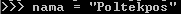
\includegraphics[width=0.45\textwidth]{figures/2/penulisanvariabel.PNG}}
	\caption{Penulisan Variabel}
	\label{fig:penulisanvariabel}
\end{figure}

Kemudian perintahkan print untuk menampilkan isi dari variabel. Caranya: \verb|Print namavariabel|
Contohnya seperti pada gambar \ref{fig:hasilperintahprint} :
\begin{figure}[!htbp]
	\centerline{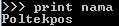
\includegraphics[width=0.55\textwidth]{figures/2/hasilperintahprint}}
	\caption{Hasil Perintah Print}
	\label{fig:hasilperintahprint}
\end{figure}

\subsection{Menghapus Variabel}
Untuk menghapus variabel caranya sangat mudah. Anda cukup menggunakan perintah del() untuk menghapus variabel yang sudah tidak dibutuhkan lagi. Perintah delete, \verb|del(namavariabel)|
Contohnya seperti pada gambar \ref{fig:perintahdel} :
\begin{figure}[!htbp]
	\centerline{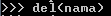
\includegraphics[width=0.40\textwidth]{figures/2/perintahdel.PNG}}
	\caption{Perintah del}
	\label{fig:perintahdel}
\end{figure}

Untuk mengecek apakah variabelnya berhasil dihapus anda bisa menggunakan perintah print seperti pada gambar \ref{fig:perintahprint}. 
\begin{figure}[!htbp]
	\centerline{
\includegraphics[width=0.55\textwidth]{figures/2/perintahprint.PNG}}
	\caption{Perintah Print}
	\label{fig:perintahprint}
\end{figure}

Jika hasilnya seperti gambar \ref{fig:afterdelete} maka variabel telah berhasil dihapus.
\begin{figure}[!htbp]
	\centerline{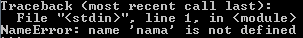
\includegraphics[width=0.75\textwidth]{figures/2/afterdelete.PNG}}
	\caption{Hasil perintah print setelah variabel di delete}
	\label{fig:afterdelete}
\end{figure}

\section{Input Output User}
Input adalah masukan yang anda berikan kepada sebuah program dan system akan memproses lalu menampilkan ouputnya.

\subsection{Cara mengambil input pada keyboard}
Di dalam python sudah terdapat fungsi input() dan raw\_input(). input() digunakan untuk masukan bernilai angka sedangkan raw\_input untuk masukan bernilai teks.

Cara penggunaannya seperti ini \verb|nama\_variabel = input(“masukkan teks”)|

Teks yang anda masukkan akan disimpan ke nama\_variabel.

Contohnya seperti pada listing \ref{lst:iouser} :
\lstinputlisting[caption=Contoh kode input output, label={lst:iouser}]{src/2/iouser.py}

Hasilnya seperti pada gambar \ref{fig:hasilinput}:
\begin{figure}[!htbp]
	\centerline{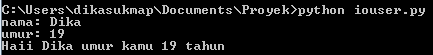
\includegraphics[width=0.85\textwidth]{figures/2/hasilinput.PNG}}
	\caption{Hasil input}
	\label{fig:hasilinput}
\end{figure}

\subsection{Menampilkan Variabel dan Teks}
Anda bisa menampilkan variabel dan teks menggunakan perintah print seperti pada listing \ref{lst:halo}
\lstinputlisting[caption=Perintah menampilkan variabel dan teks, label={lst:halo}]{src/2/halo.py}

Hasilnya seperti pada gambar \ref{fig:showvar}:
\begin{figure}[!htbp]
	\centerline{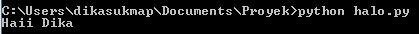
\includegraphics[width=0.85\textwidth]{figures/2/showvar.PNG}}
	\caption{Hasil menampilkan variabel dan teks}
	\label{fig:showvar}
\end{figure}

Tanda koma pada kode diatas merupakan sebuah spasi apabila kode dieksekusi.

\section{Operator Dasar}
Operator python adalah simbol yang melakukan operasi pada satu atau lebih operan. Operan adalah variabel atau nilai yang digunakan untuk melakukan operasi.
Operator pada Python dibagi menjadi beberapa jenis, yaitu :

\subsection{Operator Aritmatika}
% Please add the following required packages to your document preamble:
% \usepackage{graphicx}
\begin{table}[]
\caption{Operator Aritmatika}
\label{tab:my-table}
\resizebox{\textwidth}{!}{%
\begin{tabular}{|l|l|l|}
\hline
Operator           & Contoh      & Keterangan                                                                                                 \\ \hline
Penjumlahan +      & 3 + 1 = 4   & Menjumlahkan masing - masing bilangan                                                                      \\ \hline
Pengurangan -      & 4 - 1 = 3   & Mengurangi nilai operan di sebelah kiri menggunakan operan di sebelah kanan                                \\ \hline
Perkalian *        & 2 * 1 = 2   & Mengalikan dua bilangan                                                                                    \\ \hline
Pembagian /        & 4 / 2 = 2   & Untuk membagi operan di sebelah kiri menggunakan operan di sebelah kanan                                   \\ \hline
Sisa Bagi \%       & 13 \% 4 = 1 & Mendapatkan sisa pembagian dari operan di sebelah kiri operator ketika dibagi oleh operan di sebelah kanan \\ \hline
Pangkat **         & 6 ** 2 = 36 & Memangkatkan operan disebelah kiri operator dengan operan di sebelah kanan operator                        \\ \hline
Pembagian Bulat // & 10 // 3 = 3 & Sama seperti pembagian. Hanya saja angka dibelakang koma dihilangkan                                       \\ \hline
\end{tabular}%
}
\end{table}

Contoh penggunaannya seperti pada listing \ref{lst:aritmatika} :
\lstinputlisting[caption=Contoh operator aritmatika, label={lst:aritmatika}]{src/2/operator_aritmatika.py}

Hasilnya seperti pada gambar \ref{fig:aritmatika}:
\begin{figure}[!htbp]
	\centerline{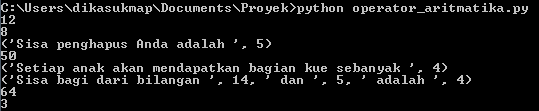
\includegraphics[width=0.85\textwidth]{figures/2/aritmatika.PNG}}
	\caption{Hasil contoh operator aritmatika}
	\label{fig:aritmatika}
\end{figure}

\subsection{Operator Perbandingan}
% Please add the following required packages to your document preamble:
% \usepackage{graphicx}
\begin{table}[]
\caption{Operator Perbandingan}
\label{tab:my-table}
\resizebox{\textwidth}{!}{%
\begin{tabular}{lll}
Operator                                    & Contoh                      & Keterangan                                                                                                       \\
Sama dengan =                               & 2 == 2                      & bernilai True Jika masing-masing operan memiliki nilai yang sama, maka kondisi bernilai benar atau True.         \\
Tidak sama dengan !=                        & 2 != 2                      & bernilai False Akan menghasilkan nilai kebalikan dari kondisi sebenarnya.                                        \\
Tidak sama dengan \textless{}\textgreater{} & 2 \textless{}\textgreater 2 & bernilai False Akan menghasilkan nilai kebalikan dari kondisi sebenarnya                                         \\
Lebih besar dari \textgreater{}             & 3 \textgreater 2            & bernilai True Jika nilai operan kiri lebih besar dari nilai operan kanan, maka kondisi menjadi benar.            \\
Lebih kecil dari \textless{}                & 2 \textless 3               & bernilai True Jika nilai operan kiri lebih kecil dari nilai operan kanan, maka kondisi menjadi benar.            \\
Lebih besar / sama dengan \textgreater{}=   & 3 \textgreater{}= 2         & bernilai True Jika nilai operan kiri lebih besar dari nilai operan kanan, atau sama, maka kondisi menjadi benar. \\
Lebih kecil / sama dengan =                 & 2 \textless{}= 3            & bernilai True Jika nilai operan kiri lebih kecil dari nilai operan kanan, atau sama, maka kondisi menjadi benar.
\end{tabular}%
}
\end{table}

Contoh penggunaannya seperti pada listing \ref{lst:perbandingan} :
\lstinputlisting[caption=Contoh operator perbandingan, label={lst:perbandingan}]{src/2/operator_perbandingan.py}

Hasilnya seperti pada gambar \ref{fig:perbandingan}:
\begin{figure}[!htbp]
	\centerline{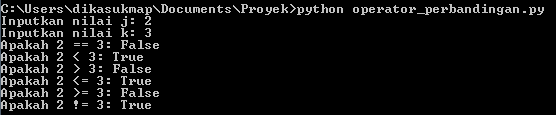
\includegraphics[width=0.85\textwidth]{figures/2/perbandingan.PNG}}
	\caption{Hasil contoh operator perbandingan}
	\label{fig:perbandingan}
\end{figure}

\subsection{Operator Penugasan}
Operator Penugasan digunakan untuk memodifikasi sebuah nilai yang ada pada variabel tertentu.
% Please add the following required packages to your document preamble:
% \usepackage{graphicx}
\begin{table}[]
\caption{Operator Penugasan}
\label{tab:my-table}
\resizebox{\textwidth}{!}{%
\begin{tabular}{lll}
Operator                        & Contoh  & Penjelasan                                                                                                                                   \\
Sama dengan =                   & A = 3   & Memberikan nilai di kanan ke dalam variabel yang berada di sebelah kiri.                                                                     \\
Tambah sama dengan +=           & A += 3  & Memberikan nilai variabel dengan nilai variabel itu sendiri ditambah dengan nilai di sebelah kanan.                                          \\
Kurang sama dengan -=           & A -= 3  & Memberikan nilai variabel dengan nilai variabel itu sendiri dikurangi dengan nilai di sebelah kanan.                                         \\
Kali sama dengan *=             & A *= 3  & Memberikan nilai variabel dengan nilai variabel itu sendiri dikali dengan nilai di sebelah kanan.                                            \\
Bagi sama dengan /=             & A /= 6  & Memberikan nilai variabel dengan nilai variabel itu sendiri dibagi dengan nilai di sebelah kanan.                                            \\
Sisa bagi sama dengan  \%=      & A \%= 3 & Memberikan nilai variabel dengan nilai variabel itu sendiri dibagi dengan nilai di sebelah kanan. Yang diambil nantinya adalah sisa baginya. \\
Pangkat sama dengan **=         & A **= 2 & Memberikan nilai variabel dengan nilai variabel itu sendiri dipangkatkan dengan nilai di sebelah kanan.                                      \\
Pembagian bulat sama dengan //= & A //= 4 & Membagi bulat operan sebelah kiri operator dengan operan sebelah kanan operator kemudian hasilnya diisikan ke operan sebelah kiri.          
\end{tabular}%
}
\end{table}

Contoh penggunaannya seperti pada listing \ref{lst:penugasan} :
\lstinputlisting[caption=Contoh operator penugasan, label={lst:penugasan}]{src/2/operator_penugasan.py}

Hasilnya seperti pada gambar \ref{fig:penugasan}:
\begin{figure}[!htbp]
	\centerline{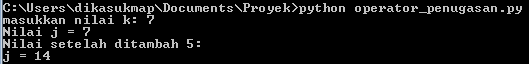
\includegraphics[width=0.85\textwidth]{figures/2/penugasan.PNG}}
	\caption{Hasil contoh operator penugasan}
	\label{fig:penugasan}
\end{figure}

\subsection{Operator Logika}
Operator logika digunakan untuk membuat operasi logika, seperti logika AND, OR, dan NOT.

\begin{table}[]
\caption{Operator Logika}
\label{tab:my-table}
\begin{tabular}{|l|l|}
\hline
Nama             & Simbol \\ \hline
Logika And       & and    \\ \hline
Logika Or        & or     \\ \hline
Negasi/kebalikan & not    \\ \hline
\end{tabular}
\end{table}

Contoh penggunaannya seperti pada listing \ref{lst:logika} :
\lstinputlisting[caption=Contoh operator logika, label={lst:logika}]{src/2/operator_logika.py}

Hasilnya seperti pada gambar \ref{fig:logika}:
\begin{figure}[!htbp]
	\centerline{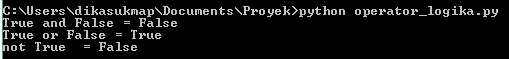
\includegraphics[width=0.85\textwidth]{figures/2/logika.PNG}}
	\caption{Hasil contoh operator logika}
	\label{fig:logika}
\end{figure}

\subsection{Operator Bitwise}
Operator bitwise digunakan untuk melakukan operasi dalam bentuk bit atau biner.

\begin{table}[]
\caption{Operator Bitwise}
\label{tab:my-table}
\begin{tabular}{|l|l|}
\hline
Nama        & Simbol                       \\ \hline
AND         & \&                           \\ \hline
OR          & |                            \\ \hline
XOR         & \textasciicircum{}           \\ \hline
Negasi      & $\sim$                       \\ \hline
Left Shift  & \textless{}\textless{}       \\ \hline
Right Shift & \textgreater{}\textgreater{} \\ \hline
\end{tabular}
\end{table}

Contoh penggunaannya seperti pada listing \ref{lst:bitwise} :
\lstinputlisting[caption=Contoh operator bitwise, label={lst:bitwise}]{src/2/operator_bitwise.py}

Hasilnya seperti pada gambar \ref{fig:bitwise}:
\begin{figure}[!htbp]
	\centerline{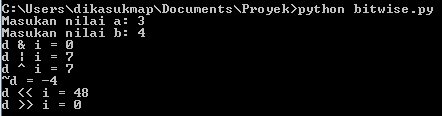
\includegraphics[width=0.85\textwidth]{figures/2/bitwise.PNG}}
	\caption{Hasil contoh operator bitwise}
	\label{fig:bitwise}
\end{figure}

\subsection{Prioritas Eksekusi Operator di Python}
Berikut adalah prioritas yang dieksekusi di dalam perintah python. Maksudnya adalah di dalam python terdapat beberapa operator dan prioritasnya masing - masing. Tabel \ref{tab:eksekusi} merupakan prioritas python dari mulai yang pertama sampai dengan yang terakhir dalam proses pengeksekusian :
\begin{table}[]
\caption{Prioritas Eksekusi Operator di Python}
\label{tab:my-table}
\begin{tabular}{|l|l|}
\hline
Operator                                                & Keterangan   \\ \hline
**                                                      & Aritmatika   \\ \hline
$\sim$,+,-                                              & Bitwise      \\ \hline
*,/,//,\%                                               & Arimatika    \\ \hline
+,-                                                     & Aritmatika   \\ \hline
\textgreater{}\textgreater{},\textless{}\textless{}     & Bitwise      \\ \hline
\&                                                      & Bitwise      \\ \hline
\textasciicircum{},|                                    & Bitwise      \\ \hline
\textless{}=,\textless{},\textgreater{},\textgreater{}= & Perbandingan \\ \hline
\textless{}\textgreater{},==,!=                         & Perbandingan \\ \hline
Err:509                                                 & Penugasan    \\ \hline
Is,is not                                               & Identitas    \\ \hline
In,not in                                               & Keanggotaan  \\ \hline
Not,or,and                                              & Logika       \\ \hline
\end{tabular}
\end{table}

\section{Perulangan / Loop}
Secara umum, perintah pada bahasa pemrograman Python akan dijalankan secara berurutan. Pernyataan pertama dalam sebuah fungsi dijalankan pertama, lalu diikuti oleh yang kedua, dan seterusnya. Tetapi akan ada situasi dimana Anda harus menulis banyak kode, dimana kode tersebut sangat banyak. Jika dilakukan secara manual maka Anda hanya akan membuang-buang waktu dan tenaga. Untuk itu Anda perlu menggunakan pengulangan atau loop di dalam bahasa pemrograman Python.

Di dalam bahasa pemrograman Python pengulangan dibagi menjadi 3 bagian, yaitu :
\subsection{While Loop}
Pada while loop pernyataan akan dieksekusi berkali-kali selama kondisi bernilai benar atau true.

Contoh penggunaannya seperti pada listing \ref{lst:whileloop} :
\lstinputlisting[caption=Koding while loop, label={lst:whileloop}]{src/2/whileloop.py}

\subsection{For Loop}
For Loop memiliki kemampuan untuk mengulangi item dari urutan apapun,misalnya string atau list.

Contoh penggunaannya seperti pada listing \ref{lst:forloop} :
\lstinputlisting[caption=Koding for loop, label={lst:forloop}]{src/2/forloop.py}
 
\subsection{Nested Loop} 
Nested loop memungkinkan terjadi sebuah pengulangan di dalam pengulangan lainnya.

Contoh penggunaannya seperti pada listing \ref{lst:nestedloop} :
\lstinputlisting[caption=Koding nested loop, label={lst:nestedloop}]{src/2/nestedloop.py}

\section{Kondisi}
\subsection{Kondisi IF}
Pada saat pengambilan keputusan (kondisi if) digunakan untuk mengantisipasi kondisi yang akan terjadi saat program dijalankan.Dan akan menentukan tindakan apa yang akan diambil sesuai dengan kondisi program pada saat dieksekusi.

Pada python ada beberapa kondisi diantaranya adalah if, else, dan elif. Kondisi if hanya bisa digunakan pada saat kondisi benar saja.

Contoh penggunaannya seperti pada listing \ref{lst:kondisiif} :
\lstinputlisting[caption=Koding kondisi if, label={lst:kondisiif}]{src/2/kondisiif.py}

Dari contoh tersebut, jika if petama dijalankan maka akan menampilkan “Selamat Ulang Tahun” sebanyak 1 kali, di statement ke 2 perintah print("Selamat Ulang Tahun") tidak akan dieksekusi karena statement bernilai salah.

\subsection{Kondisi IF Else}
Pengambilan kondisi IF Else tidak hanya mengeksekusi jika program yang telah ditetapkan bernilai benar, tetapi kondisi IF Else juga menentukan tindakan apa yang diambil jika sebuah program bernilai salah atau tidak sesuai.
Di dalam kondisi IF Else, perintah IF akan dijalankan jika pernyataan yang dieksekusi benar. Sedangkan jika pernyataan yang dieksekusi salah maka yang akan dijalankan adalah perintah Else.

Contoh penggunaannya seperti pada listing \ref{lst:kondisiifelse} :
\lstinputlisting[caption=Koding kondisi if else, label={lst:kondisiifelse}]{src/2/kondisiifelse.py}

Pada program diatas pernyataan bernilai salah, maka yang akan dieksekusi adalah perintah else dan akan menampilkan “Maaf anda tidak ulang tahun hari ini”.

\subsection{Kondisi Elif}
Kondisi if elif merupakan percabangan logikan dari “kondisi if”. Dengan Elif anda bisa membuat kondisi program menjadi banyak pilihan. Dan kondisi ini akan menyeleksi kemungkinan yang akan terjadi. Kondisi ini memiliki banyak pilihan, ini merupakan perbedaan dari kondisi elif dan kondisi if else.

Contoh penggunaannya seperti pada listing \ref{lst:kondisielif} :
\lstinputlisting[caption=Koding kondisi elif, label={lst:kondisielif}]{src/2/kondisielif.py}

Karena pernyataan diatas adalah hari minggu maka akan dieksekusi pada saat hari minggu dan akan menampilkan “ Saya akan libur”.

\section{Pembacaan Error}
Pada saat membuat suatu program, terkadang program tidak berjalan seperti yang  diinginkan. Anda harus mengetahui error apa yang terjadi dengan program yang telah dibuat. Berikut adalah 2 macam error yang terjadi pada python.
\subsection{Kesalahan sintak} 
Biasanya yang paling mudah dikenali, kesalahan sintaksis terjadi ketika Anda membuat kesalahan ketik. Tidak mengakhiri pernyataan if dengan titik dua adalah contoh kesalahan sintak, seperti salah mengeja kata kunci Python (mis. Menggunakan whille alih-alih sementara). Kesalahan sintak biasanya muncul pada waktu kompilasi dan dilaporkan oleh interpreter. 
Contoh penggunaannya seperti pada listing \ref{lst:error} :
\lstinputlisting[caption=Koding kesalahan sintak, label={lst:error}]{src/2/error.py}

Hasilnya seperti pada gambar \ref{fig:error}:
\begin{figure}[!htbp]
	\centerline{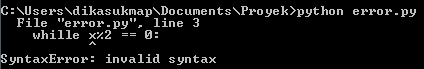
\includegraphics[width=0.85\textwidth]{figures/2/error.PNG}}
	\caption{Hasil menangkap pengecualian khusus}
	\label{fig:error}
\end{figure}
Kesalahan terdapat pada “whille”, perintah tersebut harusnya tidak menggunakan doubel l tetapi “while”.

\subsection{Kesalahan Logika}
Juga disebut kesalahan semantik, kesalahan logis menyebabkan program berperilaku tidak benar, tetapi mereka biasanya tidak crash program. Tidak seperti program dengan kesalahan sintaks, program dengan kesalahan logika dapat dijalankan, tetapi tidak beroperasi sebagaimana dimaksud. 

Pertimbangkan contoh kesalahan logis seperti pada listing \ref{lst:kesalahanlogika}:
\lstinputlisting[caption=Koding kesalahan logika, label={lst:kesalahanlogika}]{src/2/kesalahanlogika.py}

Contoh di atas harus menghitung rata-rata dari dua angka yang dimasukkan pengguna. Tetapi, karena urutan operasi dalam aritmatika (pembagian dievaluasi sebelum penambahan) program tidak akan memberikan jawaban yang benar seperti pada gambar \ref{fig:salahlogika}:
\begin{figure}[!htbp]
	\centerline{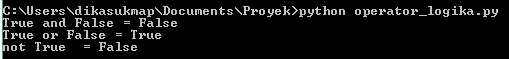
\includegraphics[width=0.85\textwidth]{figures/2/salahlogika.PNG}}
	\caption{Hasil program kesalahan logika}
	\label{fig:salahlogika}
\end{figure}

Untuk memperbaiki masalah ini, cukup menambahkan tanda kurung: z = (x + y) / 2
Ini adalah hasil yang benar seperti pada gambar \ref{fig:benarlogika}:
\begin{figure}[!htbp]
	\centerline{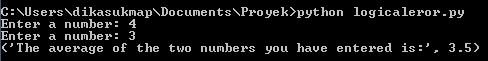
\includegraphics[width=0.85\textwidth]{figures/2/benarlogika.PNG}}
	\caption{Hasil setelah di benarkan}
	\label{fig:benarlogika}
\end{figure}

\section{Try to Except/pengecualian}
Python memiliki banyak exceptions bawaan yang memaksa program Anda untuk menghasilkan kesalahan ketika ada sesuatu yang salah di dalamnya. Ketika exceptions ini terjadi, itu menyebabkan proses saat ini berhenti dan meneruskannya ke proses panggilan sampai ditangani. Jika tidak ditangani, program ini akan macet.

Misalnya, jika fungsi A memanggil fungsi B yang pada gilirannya memanggil fungsi C dan pengecualian terjadi di fungsi C. Jika tidak ditangani dalam C, pengecualian beralih ke B dan kemudian ke A. Jika tidak pernah ditangani, pesan kesalahan dilemparkan dan program ini terhenti secara tiba-tiba.

\subsection{Menangkap Pengecualian dengan Python}
Dalam Python, pengecualian dapat ditangani menggunakan pernyataan coba. Operasi kritis yang dapat meningkatkan pengecualian ditempatkan di dalam klausa coba dan kode yang menangani pengecualian ditulis dalam kecuali klausa.

Contoh penggunaannya seperti pada listing \ref{lst:exception} :
\lstinputlisting[caption=Koding exception, label={lst:exception}]{src/2/exception.py}

Hasilnya seperti pada gambar \ref{fig:exception}:
\begin{figure}[!htbp]
	\centerline{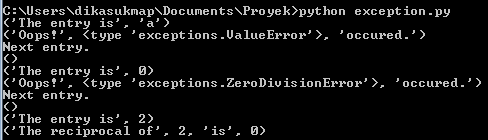
\includegraphics[width=0.85\textwidth]{figures/2/exception.PNG}}
	\caption{Hasil try to except}
	\label{fig:exception}
\end{figure}

Dalam program ini, anda harusi mengulang sampai pengguna memasukkan bilangan bulat yang memiliki timbal balik yang valid. Bagian yang dapat menyebabkan pengecualian ditempatkan di dalam blok try.

Jika tidak ada pengecualian terjadi, kecuali blok dilewati dan aliran normal berlanjut. Tetapi jika ada pengecualian terjadi, itu ditangkap oleh blok kecuali. System mencetak nama pengecualian menggunakan fungsi ex\_info () di dalam modul sys dan meminta pengguna untuk mencoba lagi. Anda dapat melihat bahwa nilai 'a' dan '1,3' menyebabkan ValueError dan '0' menyebabkan ZeroDivisionError.

\subsection{Menangkap Pengecualian Khusus dengan Python}
Dalam contoh di atas, pengecualian dalam klausa kecuali tidak disebutkan. Ini bukan praktik pemrograman yang baik karena akan menangkap semua pengecualian dan menangani setiap kasus dengan cara yang sama. Anda dapat menentukan pengecualian mana yang dikecualikan klausa kecuali.

Klausa coba dapat memiliki sejumlah kecuali klausa untuk menanganinya secara berbeda tetapi hanya satu yang akan dieksekusi jika terjadi pengecualian. Anda bisa menggunakan tupel nilai untuk menentukan beberapa pengecualian dalam klausa kecuali. 

Contoh penggunaannya seperti pada listing \ref{lst:specialexception} :
\lstinputlisting[caption=Koding special exception, label={lst:specialexception}]{src/2/specialexception.py}

\subsection{Meningkatkan Pengecualian}
Dalam pemrograman Python, pengecualian dimunculkan ketika kesalahan yang sesuai terjadi pada waktu berjalan, tetapi dapat dengan paksa menaikkannya menggunakan peningkatan kata kunci. Anda juga bisa memberikan nilai secara opsional pada pengecualian untuk mengklarifikasi mengapa pengecualian itu dinaikkan.

Contoh penggunaannya seperti pada listing \ref{lst:upexception} :
\lstinputlisting[caption=Koding meningkatkan pengecualian, label={lst:upexception}]{src/2/upexception.py}

\subsection{Try Finally}
Pernyataan coba dengan Python dapat memiliki klausa finally opsional. Klausa ini dieksekusi apa pun yang terjadi, dan umumnya digunakan untuk melepaskan sumber daya eksternal. Misalnya, anda dapat terhubung ke pusat data jarak jauh melalui jaringan atau bekerja dengan file atau bekerja dengan Graphical User Interface (GUI). 

Dalam semua keadaan ini, anda harus membersihkan sumber daya yang pernah digunakan, apakah itu berhasil atau tidak. Tindakan-tindakan ini (menutup file, GUI atau memutuskan sambungan dari jaringan) dilakukan pada klausa terakhir untuk menjamin eksekusi.

Contoh penggunaannya seperti pada listing \ref{lst:tryfinnaly} :
\lstinputlisting[caption=Koding try finnaly, label={lst:tryfinnaly}]{src/2/tryfinnaly.py}

Tipe konstruksi ini memastikan file ditutup bahkan jika pengecualian terjadi.

\chapter{Akuisisi Data Menggunakan Sensor EEG}
\section{Membuat Fungsi Dalam Satu File dan Cara Menggunakannya}
Pada bagian ini terdapat tutorial cara membuat function yang berhubungan dengan “Akuisisi Data Menggunakan Sensor EEG”. Di bagian awal ini terdapat beberapa function yang disipan dalam satu file diantaranya adalah function untuk membuat tampilan, tampilan yang ada di tutorial ini terbagi ke dalam :
\begin{enumerate}
\item Membuat tampilan untuk mencari file.
\item Membuat tampilan untuk memilih file.
\item Membuat tampilan untuk mengubah ke line graph.
\item Membuat tampilan untuk mengubah ke bar graph.
\item Membuat tampilan “file tidak ada” jika file belum dipilih.
\end{enumerate}
Setelah itu ada function untuk :
\begin{enumerate} 
\item memilih file.
\item mengconvert file ke line graph.
\item Mengkonversi file ke bar graph.
\end{enumerate}
Pada bagian ini function akan dieksekusi oleh satu fungsi dalam file yang sama.
\subsection{Function untuk membuat tampilan awal}
Seperti pada listing \ref{lst:tampilanawal}:
\lstinputlisting[caption=Tampilan awal, label={lst:tampilanawal}]{src/3/tampilanawal.py}

Langkah pertama membuat tampilan
\begin{enumerate}
\item Membuat tampilan untuk mencari file.
Seperti pada listing \ref{lst:mencarifile}:
\lstinputlisting[caption=Tampilan untuk mencari file, label={lst:mencarifile}]{src/3/mencarifile.py}

\item Membuat tampilan untuk memilih file.
Seperti pada listing \ref{lst:memilihfile}:
\lstinputlisting[caption=Tampilan untuk memilih file, label={lst:memilihfile}]{src/3/memilihfile.py}

\item Membuat tampilan untuk mengubah ke line graph.
Seperti pada listing \ref{lst:linegraph}:
\lstinputlisting[caption=Tampilan line graph, label={lst:linegraph}]{src/3/linegraph.py}

\item Membuat tampilan untuk mengubah ke bar graph.
Seperti pada listing \ref{lst:bargraph}:
\lstinputlisting[caption=Tampilan bar graph, label={lst:bargraph}]{src/3/bargraph.py}

\item Kemudian function untuk memilih file.
Seperti pada listing \ref{lst:memilihfile2}:
\lstinputlisting[caption=Tampilan untuk memilih file, label={lst:memilihfile2}]{src/3/memilihfile2.py}
\begin{itemize}
\item Buat askopenfilename() yang bertujuan untuk memberikan pertanyaan file mana yang akan dipilih. 
\item Value nya dibuat float dengan menggunakan method split agar dapat mengembalikan lagi string line yang dipanggil.
\item Membuat function open agar bisa menampilkan menu open file.
\item Didefinisikan menjadi return jika file tidak ada dan bermaksud agar perintah tersebut bisa diulang-ulang.
\item Membuat x.append dan y.append untuk value di sumbu x dan sumbu y.
\item Membuat print file sudah tersedia dengan self dengan value “file sudah tersedia”.
\end{itemize}

\item Membuat function Line Graph.
Seperti pada listing \ref{lst:flinegraph}:
\lstinputlisting[caption=Tampilan function line graph, label={lst:flinegraph}]{src/3/flinegraph.py}
\begin{itemize}
\item Definisikan line\_graph menjadi self.
\item Membuat plt.figure dan variable num dengan value line graph dan file graph to converter untuk mengconvert data ke graph.
\item Buat plt.plot dengan value maker sebagai tanda sumbu x dan sumbu y.
\item Buat plt.xlabel sebagai title yang memberitahu panjang gelombang.
\item Buat plt.xlabel sebagai title yang memberitahu banyak gelombang.
\item Pada bagian ini data dibuat ke plt atau plot karena data akan disajikan ke dalam bentuk grafik.
\item Masing-masing plot didefinisikan sehingga tampilan grafik akan sesuai dan dapat dimengerti.
\item Buat plt.show untuk menampilkan hasil.
\end{itemize}

\item Kemudian mendefinisikan bar graph.
Seperti pada listing \ref{lst:fbargraph}:
\lstinputlisting[caption=Tampilan function bar graph, label={lst:fbargraph}]{src/3/fbargraph.py}
\begin{itemize}
\item Definisikan bar\_graph menjadi self.
\item Membuat plt.figure dan variable num dengan value line graph dan file graph to converter untuk mengconvert data ke graph.
\item Buat plt.plot dengan value maker sebagai tanda sumbu x dan sumbu y.
\item Buat plt.xlabel sebagai title yang memberitahu panjang gelombang.
\item Buat plt.xlabel sebagai title yang memberitahu banyak gelombang.
\item Pada bagian ini data dibuat ke plt atau plot karena data akan disajikan ke dalam bentuk grafik.
\item Masing-masing plot didefinisikan sehingga tampilan grafik akan sesuai dan dapat dimengerti.
\item Buat plt.show untuk menampilkan hasil.
\end{itemize}
\end{enumerate}

\section{Membuat Fungsi Pada File Terpisah Dari Cara Penggunaannya}
Pada bagian ini akan diberitahu bagaimana cara membuat function secara terpisah dalam file yang berbeda-beda tetapi dapat dijalankan oleh satu function. Function tersebut diantaranya:
\begin{enumerate}
\item Function membuka dan membaca file.
\item Function Untuk Menjalankan.
\item Function Menampilkan Data
\item Function Untuk Menampilkan Gelombang.
\item Function Menampilkan Gelombang Dengan Marker.
\item Function Membuat Titile Pada Grafik.
\item Function Membuat Keterangan Pada Sumbu X.
\item Function Membuat Keterangan Pada Sumbu Y.
\item Membuat fungsi untuk menampilkan row di sumbu x dan sumbu y.
\item Function Membuat warna pada row.
\item Membuat scatter
\end{enumerate}

Pada bagian dua, fungsi dibuat secara terpisah pada file yang berbeda-beda dan hanya dapat menjalankan fungsi itu saja tidak bisa berbarengan dengan fungsi yang lain. Dan perintah untuk menjalankannya ada di dalam fungsi tersebut.
\begin{enumerate}
\item Function membuka dan membaca file.
Seperti pada listing \ref{lst:membacafile}:
\lstinputlisting[caption=Tampilan function membuka dan membaca file, label={lst:membacafile}]{src/3/membacafile.py}
\begin{itemize}
\item Buat f sebagai objek/variable yang menampung isi file. 
\item Kemudian pilih file yang akan diambil sebagai data.
\item Buat print dan f.read agar data kemudian dibaca dan dicetak.
\end{itemize}

\item Function Untuk Menjalankan.
Seperti pada listing \ref{lst:main}:
\lstinputlisting[caption=main.py, label={lst:main}]{src/3/main.py}
\begin{itemize}
\item Pada bagian ini awalnya kita mengimport mindwave, maksudnya adalah agar dapat mengambil data di alat pembaca sinyal. 
\item Setelah itu membuat variable headset yang berisikan data yang ada di computer, headset tadi kita isi dengan COM4 sesuai dengan computer yang anda gunakan.

Seperti pada listing \ref{lst:com}:
\lstinputlisting[caption=Pilih COM, label={lst:com}]{src/3/com.py}

\item Setelah itu membuat fungsi koneksi atau menghubungkan
Seperti pada listing \ref{lst:koneksi}:
\lstinputlisting[caption=Koneksi, label={lst:koneksi}]{src/3/koneksi.py}

\item Kita definisikanJika data di mindwave belum terhubung maka laptop akan mencoba menghubungkan kembali, jika sudah ada maka akan muncul “connected”.
\end{itemize}

\item Function Menampilkan Data
Seperti pada listing \ref{lst:tampildata}:
\lstinputlisting[caption=Function Menampilkan Data, label={lst:tampildata}]{src/3/tampildata.py}
\begin{itemize}
\item Membuat img = img.open sebagai function untuk memilih gambar, kemudian dipilih gambar yang akan ditampilkan.
\item Membuat variable draw.
\item Data diambil dan dimasukan.
\item Data yang ada akan diimport ke dalam bentuk gambar dan ditampilkan.
\end{itemize}

\item Function Untuk Menampilkan Gelombang.
Seperti pada listing \ref{lst:tampilgelombang}:
\lstinputlisting[caption=Function Menampilkan Gelombang, label={lst:tampilgelombang}]{src/3/tampilgelombang.py}
\begin{itemize}
\item Pertama-tama import dulu data matplotlib menjadi plot agar mudah mendefinisikan data menjadi sebuah plot. 
\item Setelah itu buatlah variable plot agar dapat membaca file csv.
\item Csv.reader agar python dapat membaca format csv.
\item Kemudian buat plt.show agar data gelombang dalam bentuk grafik dapat ditampilkan.
\end{itemize}

\item Function Menampilkan Gelombang Dengan Marker.
Seperti pada listing \ref{lst:maker}:
\lstinputlisting[caption=Function Menampilkan Gelombang Dengan Maker, label={lst:maker}]{src/3/maker.py}
\begin{itemize}
\item Pertama-tama import dulu data matplotlib menjadi plot agar mudah mendefinisikan data menjadi sebuah plot.
\item Setelah itu buatlah variable plot agar dapat membaca file csv.
\item Kemudian buat fungsi plot dan isi valuenya dengan (x, marker=’o’) untuk membuat sumbu x dan o.
\item Kemudian buat plt.show agar data gelombang dalam bentuk grafik dapat ditampilkan.
\end{itemize}

\item Function Membuat Title Pada Grafik.
Seperti pada listing \ref{lst:title}:
\lstinputlisting[caption=Function Membuat Title Pada Grafik, label={lst:title}]{src/3/title.py}
\begin{itemize}
\item Pertama-tama import dulu data matplotlib menjadi plot agar mudah mendefinisikan data menjadi sebuah plot. 
\item Setelah itu buatlah variable plot agar dapat membaca file csv.
\item Kemudian buat fungsi plot da nisi valuenya dengan (x, marker=’o’) untuk membuat sumbu x dan o.
\item Kemudian buat fungsi plt.title da nisi valuenya sesuai yang diinginkan.
\end{itemize}

\item Function Membuat Keterangan Pada Sumbu X.
Seperti pada listing \ref{lst:xlabel}:
\lstinputlisting[caption=xlabel, label={lst:xlabel}]{src/3/xlabel.py}
\begin{itemize}
\item Pertama-tama import dulu data matplotlib menjadi plot agar mudah mendefinisikan data menjadi sebuah plot. 
\item Setelah itu buatlah variable plot agar dapat membaca file csv.
\item Kemudian buat fungsi plot da nisi valuenya dengan (x, marker=’o’) untuk membuat sumbu x dan o.
\item Kemudian buat fungsi plt.title da nisi valuenya sesuai yang diinginkan.
\item Buat plt.xlabel untuk keterangan di sumbu x.
\end{itemize}

\item Function Pembuatan Rows dan Scatter 
Seperti pada listing \ref{lst:warnascatter}:
\lstinputlisting[caption=Warna Scatter, label={lst:warnascatter}]{src/3/warnascatter.py}
\begin{itemize}
\item Pertama-tama import dulu data matplotlib menjadi plot agar mudah mendefinisikan data menjadi sebuah plot. 
\item Setelah itu buatlah variable plot agar dapat membaca file csv.
\item Kemudian buat fungsi plot da nisi valuenya dengan (x, marker=’o’) untuk membuat sumbu x dan o.
\item Setelah itu buat fungsi plt.title untuk judul di atas.
\item Buat plt.xlabel untuk keterangan di sumbu x.
\item Buat plt.ylabel untuk keterangan di sumbu y.
\item Setelah itu buat fungsi x.append untuk sumbu x.
\item Buat fungsi y.append untuk sumbu y agar di setiap sumbu terdapat row tingkatan jumlah data.
\item Buat plt.hist dengan value facecolor dan definisikan warnanya.
\item Setelah itu membuat fungsi scatter untuk sumbu x.
\item Setelah itu membuat fungsi scatter untuk sumbu y agar gelombang dan row dapat dibaca dengan pas.
\item Tambahkan scatter facecolor pada x dan y.
\end{itemize}
\end{enumerate}

\section{Membuat Kelas dan Cara Instalasi Kelas Pada Program Utama}
Pada bagian ini akan dibahas cara membuat kelas dan cara memanggil kelas tersebut pada program utama. Pertama-tama buatlah kelas terlebih dahulu.

Seperti pada listing \ref{lst:class}:
\lstinputlisting[caption=Membuat Kelas, label={lst:class}]{src/3/class.py}
	
Langkah selanjutnya buatlah dua objek yang sama-sama memanggil class tersebut.
Seperti pada listing \ref{lst:object}:
\lstinputlisting[caption=Membuat Objek Kelas, label={lst:object}]{src/3/object.py}

\section{Hasil Pengujian}
\subsection{Tampilan awal}
Hasilnya seperti pada gambar \ref{fig:tampilanawal}:
\begin{figure}[!htbp]
	\centerline{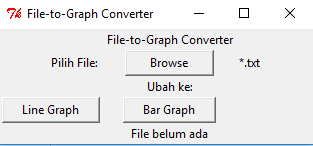
\includegraphics[width=0.85\textwidth]{figures/3/tampilanawal.PNG}}
	\caption{Tampilan awal}
	\label{fig:tampilanawal}
\end{figure}

\subsection{Tampilan Pilih File}
Hasilnya seperti pada gambar \ref{fig:tampilanpilih}:
\begin{figure}[!htbp]
	\centerline{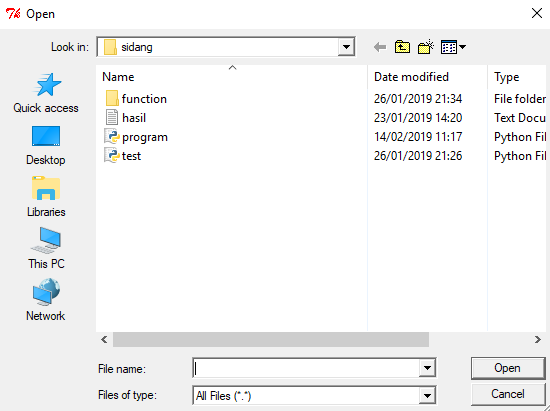
\includegraphics[width=0.85\textwidth]{figures/3/tampilanpilih.PNG}}
	\caption{Tampilan pilih file}
	\label{fig:tampilanpilih}
\end{figure}

\subsection{Tampilan line graph}
Hasilnya seperti pada gambar \ref{fig:linegraph}:
\begin{figure}[!htbp]
	\centerline{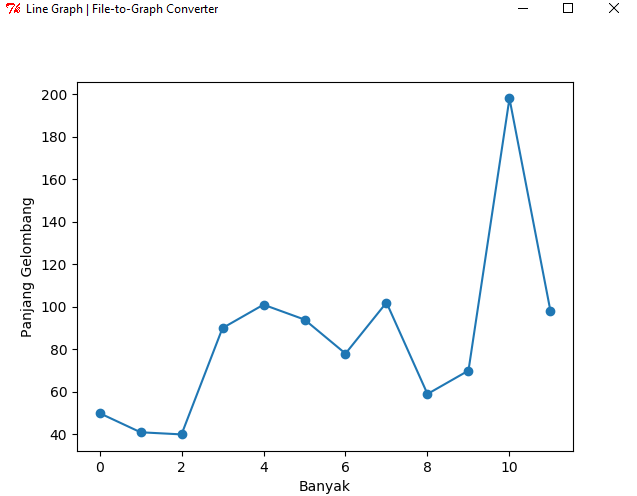
\includegraphics[width=0.85\textwidth]{figures/3/linegraph.PNG}}
	\caption{Data line graph}
	\label{fig:linegraph}
\end{figure}

\subsection{Tampilan Bar Graph}
Hasilnya seperti pada gambar \ref{fig:bargraph}:
\begin{figure}[!htbp]
	\centerline{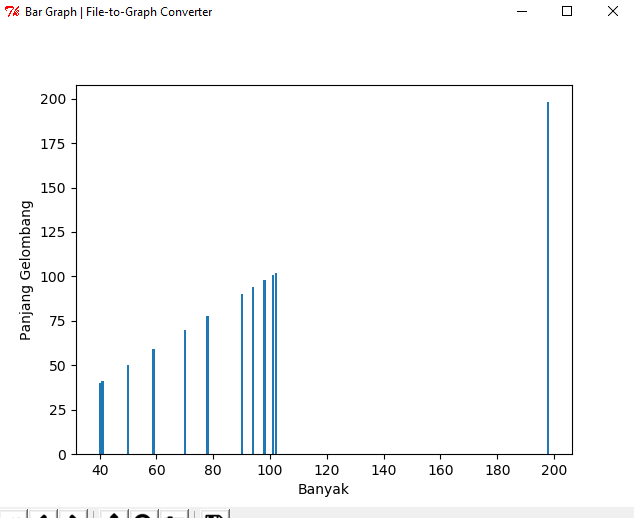
\includegraphics[width=0.85\textwidth]{figures/3/bargraph.PNG}}
	\caption{Data bar graph}
	\label{fig:bargraph}
\end{figure}

\section{PENANGANAN ERROR PADA PYTHON}
\subsection{Penanganan error}
Saat menjalankan program terkadang program tidak jalan/tidak dapat dieksekusi, untuk menangani hal tersebut harus diketahui terlebih dahulu errornya, setelah error diketahui maka program dapat dijalankan kembali. Error yang terjadi pada saat menjalankan program di python terbagi menjadi dua yaitu error pada penulisan syntax dan error pada logika yang diperintahkan dalam program. Karena suatu python tidak akan mengerti perintah yang dimasukkan jika program tersebut terdapat kesalahan dan tidak dapat dimengerti oleh computer.

\begin{enumerate}
\item Kesalahan syntax

Kesalahan syntax biasanya terjadi dalam kesalahan penulisan, jika syntax tidak ada dalam python dan tidak bisa dipahami maka python akan menunjukkan adanya kesalahan dalam program tersebut. Untuk mengatasi error dalam penulisan syntax maka pembuat program harus lebih teliti lagi dalam pengetikan saat memberikan perintah di python.

Berikut adalah contoh error yang terjadi karena kesalahan syntax seperti pada gambar \ref{fig:salahsintak}
\begin{figure}[!htbp]
	\centerline{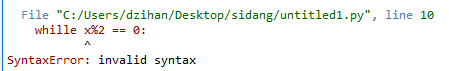
\includegraphics[width=0.85\textwidth]{figures/3/salahsintak.PNG}}
	\caption{Kesalahan sintak}
	\label{fig:salahsintak}
\end{figure}
	
Gambar \ref{fig:salahsintak} adalah contoh error yang terjadi yang disebabkan oleh kesalahan dalam penulisan syntax. Hal tersebut terjadi karena dalam program tersebut terdapat ‘kata’ atau perintah yang tidak dapat dipahami oleh komputer.

Untuk menangani hal tersebut maka periksa lagi lagi atau klik errornya seperti pada listing \ref{lst:syntaxsolution}:
\lstinputlisting[caption=Solusi Kesalahan Sintak, label={lst:syntaxsolution}]{src/3/syntaxsolution.py}

\item Kesalahan logika
Selain kesalahan syntax ada juga kesalahan logika. Kesalahan logika terjadi akibat terdapat logika yang tidak dapat dipahami dalam program yang dibuat seperti pada gambar \ref{fig:salahlogika}
\begin{figure}[!htbp]
	\centerline{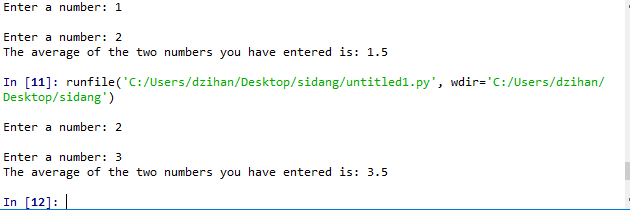
\includegraphics[width=0.85\textwidth]{figures/3/salahlogika.PNG}}
	\caption{Kesalahan logika}
	\label{fig:salahlogika}
\end{figure}

Untuk memperbaiki error tersebut cukup dengan menambahkan tanda kurung dalam rumusnya seperti pada listing \ref{lst:logicsolution}:
\lstinputlisting[caption=Solusi Kesalahan Logika, label={lst:logicsolution}]{src/3/logicsolution.py}:
\end{enumerate}

\subsection{Fungsi memilih line graph}
Seperti pada listing \ref{lst:linegraph2}:
\lstinputlisting[caption=Line Graph, label={lst:linegraph2}]{src/3/linegraph2.py}

Seperti pada gambar \ref{fig:errorplt}
\begin{figure}[!htbp]
	\centerline{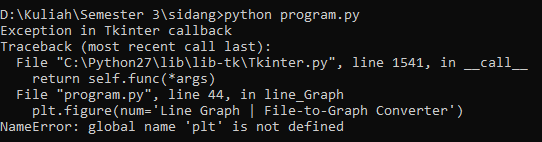
\includegraphics[width=0.85\textwidth]{figures/3/errorplt.PNG}}
	\caption{Error plt}
	\label{fig:errorplt}
\end{figure}

Pada bagian awal terdapat exeption pada bagian tkinter, karena untuk menjalankan fungsi plot diperlukan adanya sebuah import terlebih dahulu dari matplotlib agar data dapat dibaca dan dikonversi ke plot.

Pada bagian ini terdapat error yang menunjukan bahwa global name dengan nama plt tidak terdefinisikan. Dalam fungsi pengambilan data, data diharuskan diimport dulu ke plot dengan menggunakan matplotlib agar data dapat disajikan dalam bentuk plot. Agar lebih mudah didefinisikan, maka matplotlib menggunakan “as” atau alias sebagai plt. 

Untuk menangani error tersebut ada beberapa langkah yang harus dikerjakan :
\begin{enumerate}
\item Import matplotlib.pyplot
\item buat lah “as” atau alias pada bagian import matplotlib agar fungsi yang ada di line\_graph dapat mendefinisikan plt tersebut sebagai matplotlib.
\item Pada bagian fungsi line\_graph harus didefinsikan sama seperti alias yang telah ditentukan
Seperti pada listing \ref{lst:import}:
\lstinputlisting[caption=Import, label={lst:import}]{src/3/import.py}
\item Setelah dibuat langkah-langkah tersebut maka function dapat dijalankan kembali dan function line graph dapat mendefinisikan plt sebagai matplotlib.
\end{enumerate}

\subsection{Fungsi memilih file}
Seperti pada listing \ref{lst:choosefile}:
\lstinputlisting[caption=Memilih file, label={lst:choosefile}]{src/3/choosefile.py}

\begin{figure}[!htbp]
	\centerline{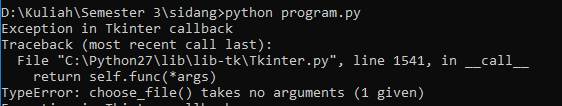
\includegraphics[width=0.85\textwidth]{figures/3/errorcf.PNG}}
	\caption{Error Choose File}
	\label{fig:errorcf}
\end{figure}
Pada gambar \ref{fig:errorcf} terdapat error exception bagian type error, yang menunjukan bahwa ada error di bagian choose file dan adanya sebuah fungsi yang dieksekusi dengan type objek yang tidak sesuai.

Untuk menangani hal tersebut perlu dibuat parameter self, jika sebuah method yang ada pada dirinya sendiri harus diawali dengan self.
Seperti pada listing \ref{lst:selfcf}:
\lstinputlisting[caption=Self Choose File, label={lst:selfcf}]{src/3/selfcf.py}

self.adaFile["text"]="File sudah tersedia!" Pada bagian ini sebelum menjalankan perintah “adaFile” dan memunculkan print “file sudah tersedia, self akan memanggil dirinya sendiri terlebih dahulu kemudia menjalankan perintah “adaFile”. Itulah kegunaan self dan hasil dari penanganan error menggunakan self membuat fungsi choose file dapat dijalankan kembali.

Seperti pada gambar \ref{fig:selfcf}
\begin{figure}[!htbp]
	\centerline{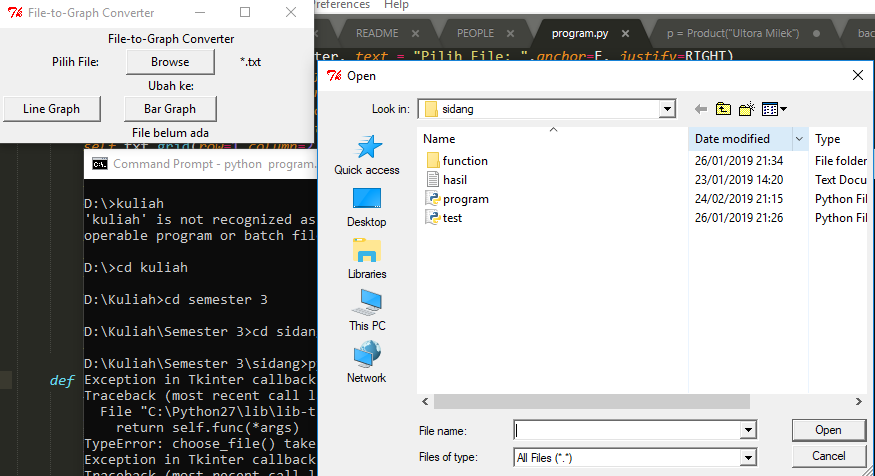
\includegraphics[width=0.85\textwidth]{figures/3/selfcf.PNG}}
	\caption{Self Choose File}
	\label{fig:selfcf}
\end{figure}

Seperti pada listing \ref{lst:file_name}:
\lstinputlisting[caption=file\_name, label={lst:file_name}]{src/3/file_name.py}

\begin{figure}[!htbp]
	\centerline{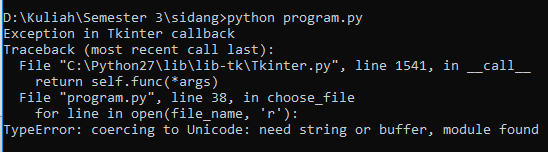
\includegraphics[width=0.85\textwidth]{figures/3/file_name.PNG}}
	\caption{Error file\_name}
	\label{fig:file_name}
\end{figure}
Pada gambar \ref{fig:file_name} memberitahu exeption yang terjadi pada fungsi memilih file, tepatnya pada bagian file\_name. Exeption yang tertera di gambar adalah TypeError yang memberitahu bahwa method tersebut membutuhkan string.

Seperti pada listing \ref{lst:openfile}:
\lstinputlisting[caption=open\_file, label={lst:openfile}]{src/3/openfile.py}
	
Pada bagian ini terdapat perintah open yang memanggil file\_name dan r, namun r disini tidak dapat ditemukan. Maka penaganan error untuk bagian ini adalah sebagai berikut :
\begin{enumerate}	
\item Definisikan r menjadi askopenfile agar r dapat menjalankan sebuah perintah. file\_name = filedialog.askopenfilename().
\end{enumerate}

\section{Tutorial Penanganan Error Pada Tkinter}
Pada pembuatan sebuah tampilan menggunakan GUI, maka harus menggunakan tkinter untuk dapat menampilkan interface berbentuk menu GUI. Dalam penggunaan tkinter sering terdapat kesalahan/error saat proses import tkinter ke python. Seperti pada gambar \ref{fig:errortkinter}
\begin{figure}[!htbp]
	\centerline{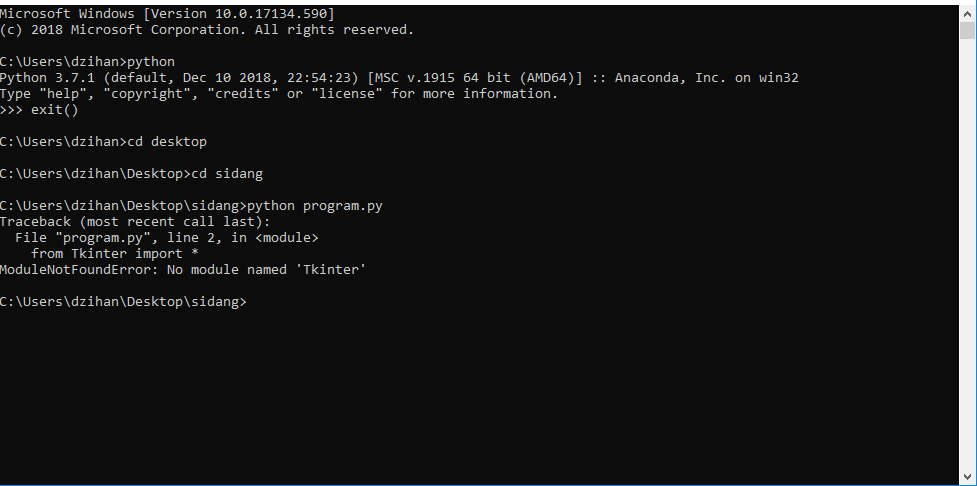
\includegraphics[width=0.85\textwidth]{figures/3/errortkinter.PNG}}
	\caption{Error Tkinter}
	\label{fig:errortkinter}
\end{figure}

Dalam kasus error tersebut python tidak dapat menampilkan program.py karena tidak terdapat modul tkinter. Dalam program.py tersebut ada source code yang diperintahkan untuk menampilkan menu GUI, dalam menu GUI tersebut terdpat fungsi-fungsi. JIka menu tidak bisa diakses maka fungsi pun tidak akan dapat dijalankan. Untuk menangani error tersebut perlu dilakukan import tkinter.
\begin{enumerate}
\item Buka cmd
\item Buka python
\item Ketik Import tkinter

Seperti pada listing \ref{lst:tkinter}:
\lstinputlisting[caption=Import Tkinter, label={lst:tkinter}]{src/3/tkinter.py}

Seperti pada gambar \ref{fig:tkinter}
\begin{figure}[!htbp]
	\centerline{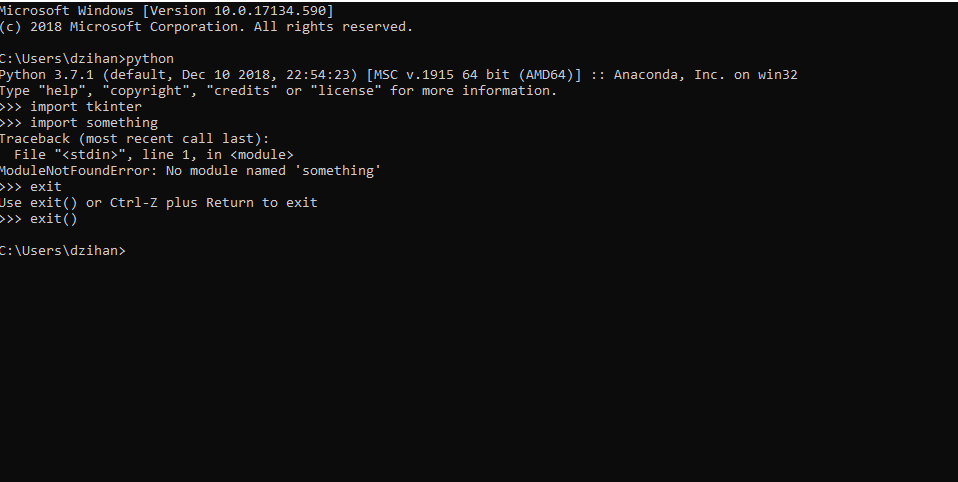
\includegraphics[width=0.85\textwidth]{figures/3/tkinter.PNG}}
	\caption{Import Tkinter}
	\label{fig:tkinter}
\end{figure}

\item Kemudian buka instalasi python yang telah didownload.
Seperti pada gambar \ref{fig:folderpython}
\begin{figure}[!htbp]
	\centerline{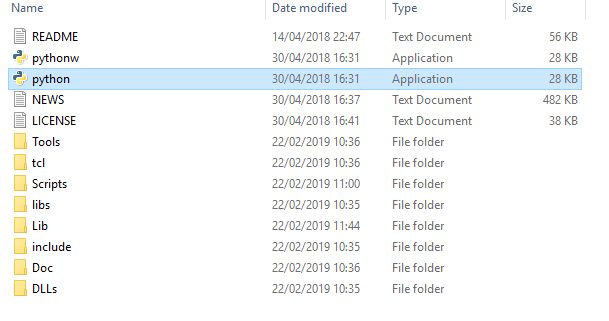
\includegraphics[width=0.85\textwidth]{figures/3/folderpython.PNG}}
	\caption{Folder Python}
	\label{fig:folderpython}
\end{figure}

\item Arahkan atau drop ke cmd
Seperti pada gambar \ref{fig:dropfolder}
\begin{figure}[!htbp]
	\centerline{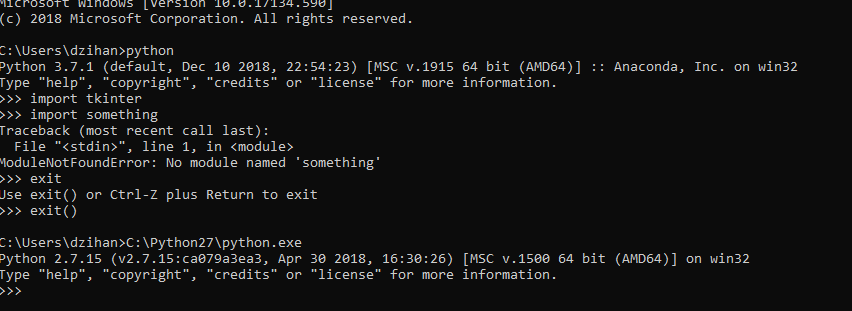
\includegraphics[width=0.85\textwidth]{figures/3/dropfolder.PNG}}
	\caption{Drop Folder}
	\label{fig:dropfolder}
\end{figure}

\item Setelah itu import kembali tkinter
\end{enumerate}

Jika cara tersebut tidak berhasil, cobalah cara lain seperti tutorial di bawah ini :
\begin{enumerate}
\item Buka folder python.
Seperti pada gambar \ref{fig:bukafolder}
\begin{figure}[!htbp]
	\centerline{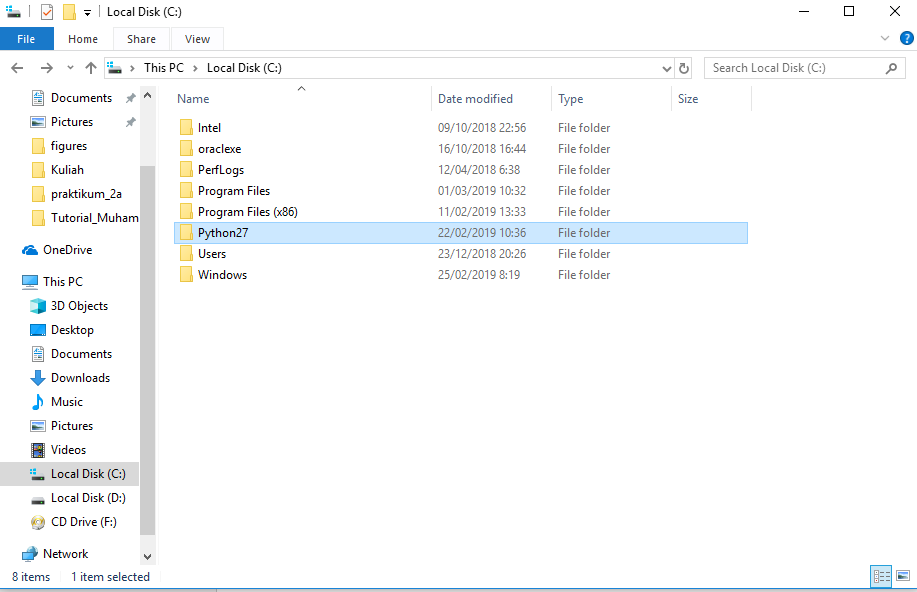
\includegraphics[width=0.85\textwidth]{figures/3/bukafolder.PNG}}
	\caption{Buka Folder Python}
	\label{fig:bukafolder}
\end{figure}

\item Buka cmd
\item Tambahkan folder python tadi ke cmd.
Seperti pada gambar \ref{fig:tambahfolder}
\begin{figure}[!htbp]
	\centerline{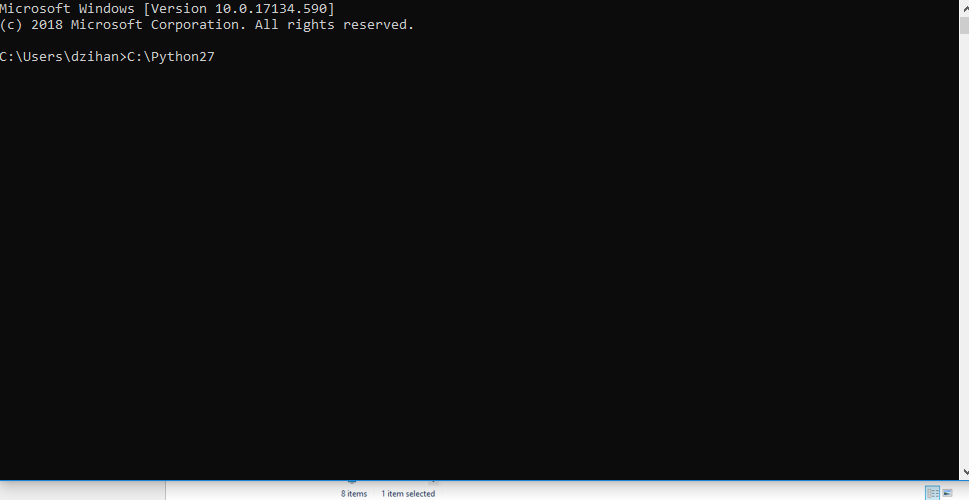
\includegraphics[width=0.85\textwidth]{figures/3/tambahfolder.PNG}}
	\caption{Tambahkan Folder}
	\label{fig:tambahfolder}
\end{figure}

\item Ketik pip install “nama modul”
Seperti pada listing \ref{lst:pipinstall}:
\lstinputlisting[caption=Pip install "nama modul", label={lst:pipinstall}]{src/3/pipinstall.py}

Seperti pada gambar \ref{fig:installmodul}
\begin{figure}[!htbp]
	\centerline{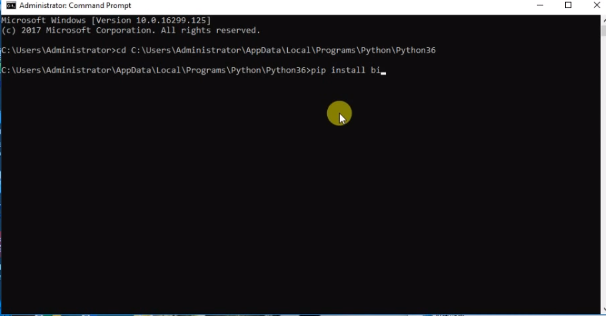
\includegraphics[width=0.85\textwidth]{figures/3/installmodul.PNG}}
	\caption{Install Modul}
	\label{fig:installmodul}
\end{figure}

\item Modul sudah tersedia
Seperti pada gambar \ref{fig:atkinter}
\begin{figure}[!htbp]
	\centerline{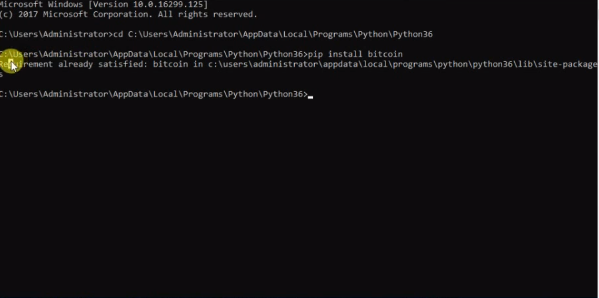
\includegraphics[width=0.85\textwidth]{figures/3/atkinter.PNG}}
	\caption{Modul sudah tersedia}
	\label{fig:atkinter}
\end{figure}
\end{enumerate}

\chapter{PYSERIAL MINDWAVE}
\section{Pyserial Mindwave}
NeuroSky Mindwave EEG adalah alat yang digunakan dalam penelitian ini dan alat terhubung ke Kode Python sebagai bahasa pemrograman yang digunakan sehingga menampilkan sinyal mentah nyata. Serta menggunakan pyserial merupakan modul Python siap-pakai dan gratis yang dibuat untuk memudahkan kita dalam membuat program komunikasi data serial RS232 dalam bahasa Python.

\section{Code Program Mindwave}
\subsection{Code Program Pyserial Function Pada Mindwave}
\begin{enumerate}
\item Berikut Codingan Function Untuk Menampilkan Gelombang Otak pada Mindwave seperti pada listing \ref{lst:gomw} : 
\lstinputlisting[caption=Function Untuk Menampilkan Gelombang Otak pada Mindwave, label={lst:gomw}]{src/4/gomw.py}
Pada listing \ref{lst:gomw}: menunjukkan adanya pemberian ukuran pada grafik gelombang otak, dan menampilkan  gelombang otak dalam grafik. Berikut gambar \ref{fig:gomw} hasil dari function menampilkan gelombang otak.
\begin{figure}[!htbp]
	\centerline{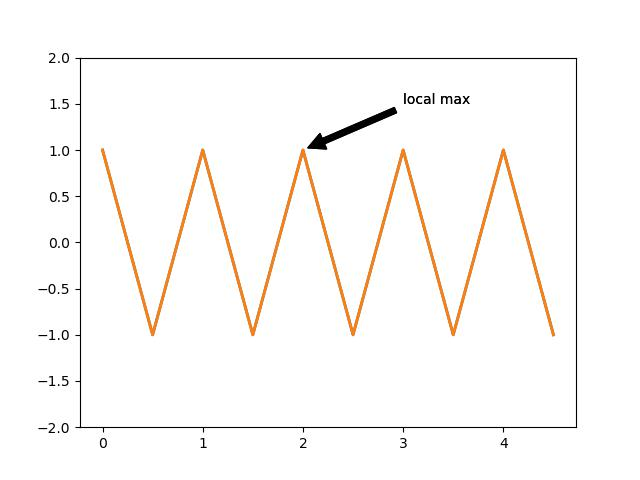
\includegraphics[width=0.85\textwidth]{figures/4/gomw.PNG}}
	\caption{function menampilkan gelombang otak}
	\label{fig:gomw}
\end{figure}

\item Codingan Function Memasukan Data Plotting Pada Mindwave seperti pada listing \ref{lst:dpmw} : 
\lstinputlisting[caption=Function Memasukan Data Plotting Otak pada Mindwave, label={lst:dpmw}]{src/4/dpmw.py}
Pada listing \ref{lst:dpmw} menunjukan bahwa adanya penambahan pada data plotting dengan memberikan judul pada grafik gelombang otak serta memberikan keterangan waktu dan voltage. Berikut hasil dari codingan pada function memasukkan data plotting seperti pada gambar \ref{fig:dpmw} :
\begin{figure}[!htbp]
	\centerline{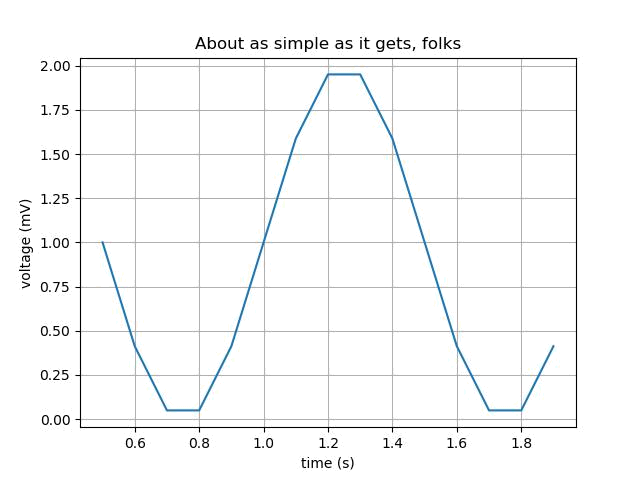
\includegraphics[width=0.85\textwidth]{figures/4/dpmw.PNG}}
	\caption{function Data Plotting pada Mindwave}
	\label{fig:dpmw}
\end{figure}

\item Code Program Function Sub.plot Pada Mindwave seperti pada listing \ref{lst:spmw} : 
\lstinputlisting[caption=Function Subplot pada Mindwave, label={lst:spmw}]{src/4/spmw.py}
Pada listing \ref{lst:spmw} menjelaskan bahwa adanya perubahan pada sub.plot mindwave ini yang menunjukkan tampilan grafik gelombang otak dengan ukuran gambar yang kecil. Berikut hasil dari codingannya seperti pada gambar \ref{fig:spmw} :
\begin{figure}[!htbp]
	\centerline{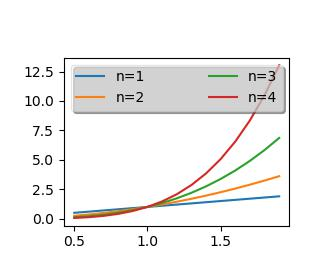
\includegraphics[width=0.85\textwidth]{figures/4/spmw.PNG}}
	\caption{function Subplot pada Mindwave}
	\label{fig:spmw}
\end{figure}

\item Code Program Function Memberikan Keterangan Waktu dan Frekuensi seperti pada listing \ref{lst:kwf} : 
\lstinputlisting[caption=Function Memberikan Keterangan Waktu dan Frekuensi, label={lst:kwf}]{src/4/kwf.py}
Pada listing \ref{lst:kwf} mejelaskan adanya penambahan function keterangan waktu dan frekuensi pada pyserial mindwave.
Berikut hasil dari codingannya seperti pada gambar \ref{fig:kwf} :
\begin{figure}[!htbp]
	\centerline{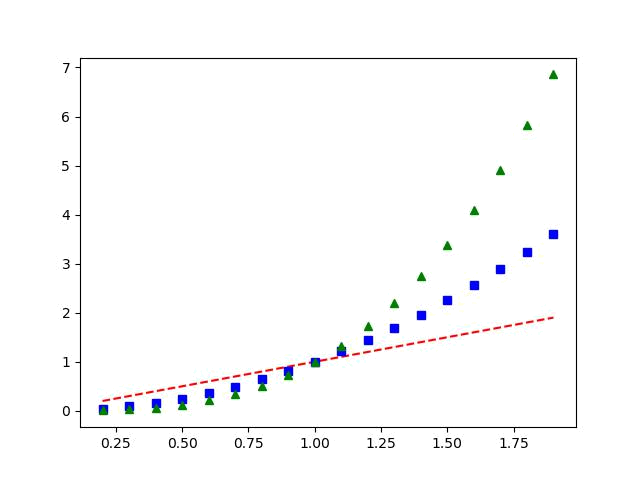
\includegraphics[width=0.85\textwidth]{figures/4/kwf.PNG}}
	\caption{Function Memberikan Keterangan Waktu dan Frekuensi}
	\label{fig:kwf}
\end{figure}

\item Code Program Function Memasukkan Rumus Pada Grafik Gelombang Otak seperti pada listing \ref{lst:rumusgrafik} : 
\lstinputlisting[caption=Function Memasukkan Rumus Pada Grafik Gelombang Otak, label={lst:rumusgrafik}]{src/4/rumusgrafik.py}
Pada listing \ref{lst:rumusgrafik} mejelaskan adanya penambahan function memasukkan rumus gelombang otak pada pyserial mindwave.
Berikut hasil dari codingannya seperti pada gambar \ref{fig:rumusgrafik} :
\begin{figure}[!htbp]
	\centerline{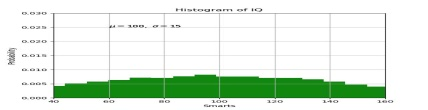
\includegraphics[width=0.85\textwidth]{figures/4/rumusgrafik.PNG}}
	\caption{Function Memasukkan Rumus Pada Grafik Gelombang Otak}
	\label{fig:rumusgrafik}
\end{figure}
\end{enumerate}

\section{Tutorial Mengatasi error Pyserial Function pada Mindwave}
\subsection{Mengenal error Dalam Program}
Pada bahasa pemrograman, terdapat bahasa yang berbasis dekstop,web,dan lain-lain. Misalnya di dalam bahasa C, setiap pernyataan harus diakhiri dengan titik koma, namun pada visual basic tidak perlu digunakan.

Saat kita menjalankan suatu program dalam  bahasa pemrograman menemukan kesalahan pada sintaks atau codingan di dalam suatu prorgam sehingga menyebabkan program tidak berjalan dengan baik.

Dilihat dari jenis kesulitan dalam memperbaiki suatu program, terdapat 3 kesalahan yaitu :
\begin{enumerate}
\item error Tata Bahasa (Sintaks)

Merupakan jenis error yang sering terjadi dalam pembuatan program. Namun error ini sangat mudah terdekteksi karena umumnya compier dari masing-masing bahasa program sebelum program  di jalankan.

\item Error Runtime

Merupakan tingkatan dimana error ini dapat terdeksi saat program dijalakan. Penyebabnya beragam, karena terjadinya kesalahan dalam proses input,serta perhitungan saat proses output.

\item Error Logika (Logical Error)

Merupakan jenis error yang sangat sulit terdeteksi karena terjadinya bukan karena kesalahan pada penulisan sintaks,melainkan dari kesalahan programmer dalam menggunakan algoritma.
\end{enumerate}

\subsection{Code error Pada Program Pyserial Mindwave}
\begin{enumerate}
\item Error no attribute
Hasilnya seperti pada gambar \ref{fig:errorna} :
\begin{figure}[!htbp]
	\centerline{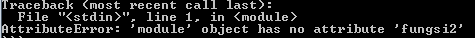
\includegraphics[width=0.85\textwidth]{figures/4/errorna.PNG}}
	\caption{Error no attribute}
	\label{fig:errorna}
\end{figure}
Jika Masih ada yang error di kodingnya. Perhatikan lagi kodingnya.

\item Error Indentation
Hasilnya seperti pada gambar \ref{fig:errori} :
\begin{figure}[!htbp]
	\centerline{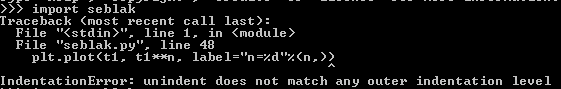
\includegraphics[width=0.85\textwidth]{figures/4/errori.PNG}}
	\caption{Error Indetation}
	\label{fig:errori}
\end{figure}
Berarti masih ada yang error dalam jarak spasi coba di sesuaikan dengan baris
Yang lain.

\item Error Parameter
Hasilnya seperti pada gambar \ref{fig:errorp1} :
\begin{figure}[!htbp]
	\centerline{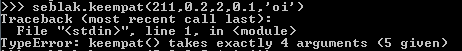
\includegraphics[width=0.85\textwidth]{figures/4/errorp1.PNG}}
	\caption{Error Parameter}
	\label{fig:errorp1}
\end{figure}
Jika terjadi error seperti di atas berarti kita memasukkan parameternya
Kelebihan  atau kekurangan. Jadi sesuaikan parameter yang anda isi dengan
Kodingan.

\item Error parameter 
Hasilnya seperti pada gambar \ref{fig:errorp2} :
\begin{figure}[!htbp]
	\centerline{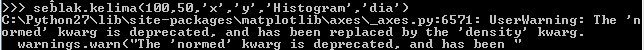
\includegraphics[width=0.85\textwidth]{figures/4/errorp2.PNG}}
	\caption{Error Parameter}
	\label{fig:errorp2}
\end{figure}
Jika terjadi seperti diatas maka cek dulu nama parameternya, kemungkinan masih terjadi   kesalahan penulisan.

\item Error Penulisan
Hasilnya seperti pada gambar \ref{fig:errorpn} :
\begin{figure}[!htbp]
	\centerline{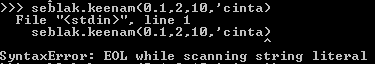
\includegraphics[width=0.85\textwidth]{figures/4/errorpn.PNG}}
	\caption{Error Penulisan}
	\label{fig:errorpn}
\end{figure}
Jika terjadi error seperti diatas, maka perhatikan penggunan tanda baca.
\end{enumerate}

%\chapter{}
%\section{Perintah Navigasi}
Perintah navigasi direktori


\chapter{PENYAJIAN DATA DALAM PENGGUNAAN MATPLOTLIB}
\section{Penjelasan Matplotlib}
Matplotlib adalah sebuah modul/librari Python yang menghasilkan gambar publikasi berguna untuk keperluan dalam penyajian pada data science. Matploblib juga bermutu di dalam berbagai format hardcopy dan lingkungan interaktif sepanjang platform. Matplotlib dapat digunakan di dalam script Python, shell Python dan ipython. Dengan matplotlib, kita dapat membuat sebuah plots, histograms, spectra, bar charts, errorchards, scatterplots, dan sebagainya. Pembuat matplotlib ialah seseorang yang bernama John D. Hunter yang pada 28 Agustus 2012 lalu meninggal dunia setelah bergelut dengan komplikasi kanker yang diidap beliau. Jasa beliau untuk Python Community sungguh sangat luar biasa (khususnya python untuk science [1].
       
\section{Pemasangan Matlotlib}
Disini saya menggunakan sistem operasi windows, sebelum anda menginstall matplotlib kita harus memasang python terlebih dahulu. Disini saya menggunakan python 2,7.

Jika kita sudah memasang python maka selanjutnya ialah kita memvalidasi python menggunakan CMD sampai tampilan seperti pada gambar \ref{fig:cmd}: 
\begin{figure}[!htbp]
	\centerline{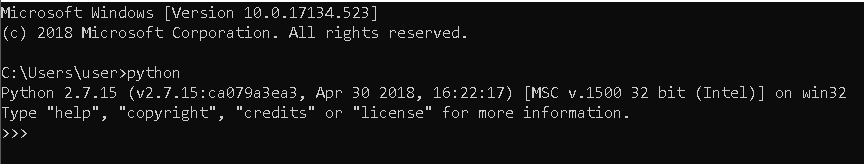
\includegraphics[width=0.85\textwidth]{figures/6/cmd.PNG}}
	\caption{Validasi Python}
	\label{fig:cmd}
\end{figure}

Jika tampilan sudah seperti gambar \ref{fig:cmd}, maka selanjutnya kita akan memasang modul matplotlib. Matplotlib dapat diinstal dengan menjalankan perintah berikut di dalam CMD, disini saya akan menggunakan pip, namun anda dapat menggunakan tool lainnya. 
\begin{figure}[!htbp]
	\centerline{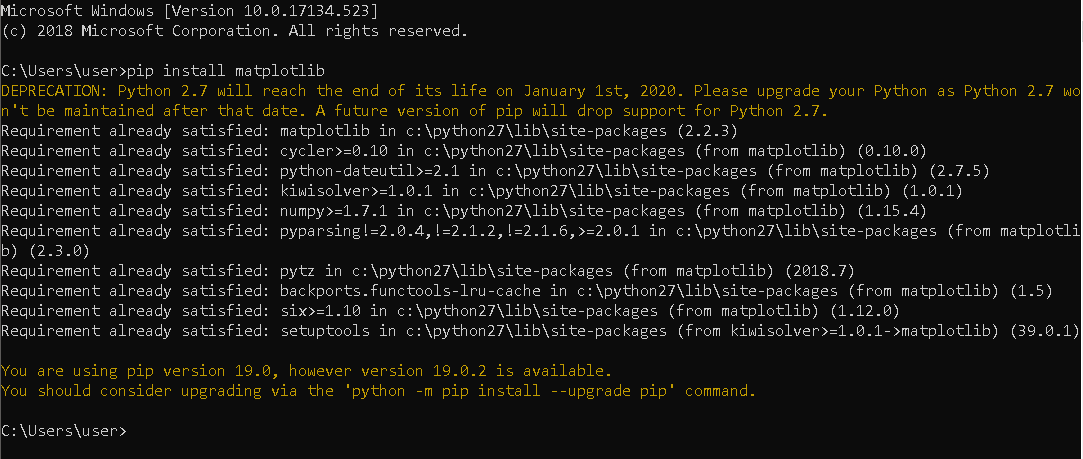
\includegraphics[width=0.85\textwidth]{figures/6/pasangmpl.PNG}}
	\caption{Pemasangan Matplotlib}
	\label{fig:pasangmpl}
\end{figure}

Jika tampilan sudah seperti gambar \ref{fig:pasangmpl}, maka matplotlib telah terpasang dan siap digunakan [2].

\section{Menggambar Plot Dasar}
Sekarang kita akan membahas tentang membuat sebuah plot dasar, atau membaca sebuah data yang berupa angka menjadi sebuah plot.
\subsection{Plot Garis}
Kita akan membahas sebuah contoh sederhana dalam menggambar sebuah plot garis menggunakan matplotlib. Dalam contoh ini, kita akan membuat sebuah garis dari data angka yang memiliki sumbu x dan y
Untuk data yang akan kita buat sebagai plot adalah sebagai berikut : 
\begin{verbatim}
x = (4,8,13,17,20)
y = (54, 67, 98, 78, 45)
\end{verbatim}

Ini dapat dilakukan dengan menggunakan seperti pada listing \ref{lst:plotgaris} : 
\lstinputlisting[caption=Skrip Plot Garis, label={lst:plotgaris}]{src/6/plotgaris.py}
Perhatikan bahwa kita menyajikan titik x dan y sebagai daftar.
Dalam contoh ini, hasilnya akan menjadi seperti pada gambar \ref{fig:plotgaris}:
\begin{figure}[!htbp]
	\centerline{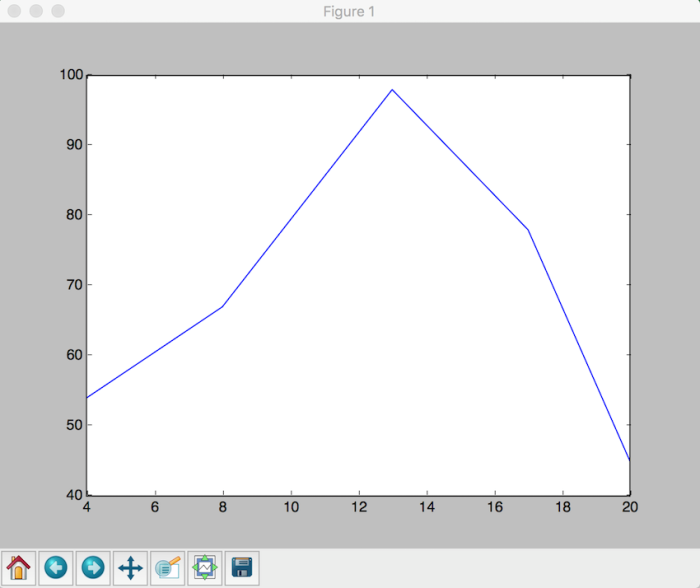
\includegraphics[width=0.85\textwidth]{figures/6/plotgaris.PNG}}
	\caption{Tampilan Plot Garis}
	\label{fig:plotgaris}
\end{figure}

Garis pada gambar di atas adalah garis default yang digambarkan untuk sebuah plot dasar, baik bentuk dan warnanya. Kita dapat memodifikasi itu dengan mengubah bentuk dan warna garis menggunakan beberapa fungsi dari dokumentasi matplotlib.

\subsection{Plot Sebaran}
Sebuah plot sebaran adalah sebuah grafik yang menunjukkan hubungan antara dua set data, di plot sebaran ini digambarkan melalui titik titik yang saling terhubung ke angka-angka yang ada di sumbu x dan y. Di dalam contoh ini, kita akan membahas menggambar sebuah plot sebaran menggunakan matplotlib.

Untuk data yang akan kita buat sebagai plot adalah sebagai berikut : 
\begin{verbatim}
x = [2,4,6,7,9,13,19,26,29,31,36,40,48,51,57,67,69,71,78,88]
y = [54,72,43,2,8,98,109,5,35,28,48,83,94,84,73,11,464,75,200,54]
\end{verbatim}
Plot sebaran dapat digambarkan menggunakan seperti pada listing \ref{lst:plotsebaran} : 
\lstinputlisting[caption=Skrip Plot Sebaran, label={lst:plotsebaran}]{src/6/plotsebaran.py}

Dalam contoh ini, hasilnya akan menjadi seperti pada gambar \ref{fig:plotsebaran}:
\begin{figure}[!htbp]
	\centerline{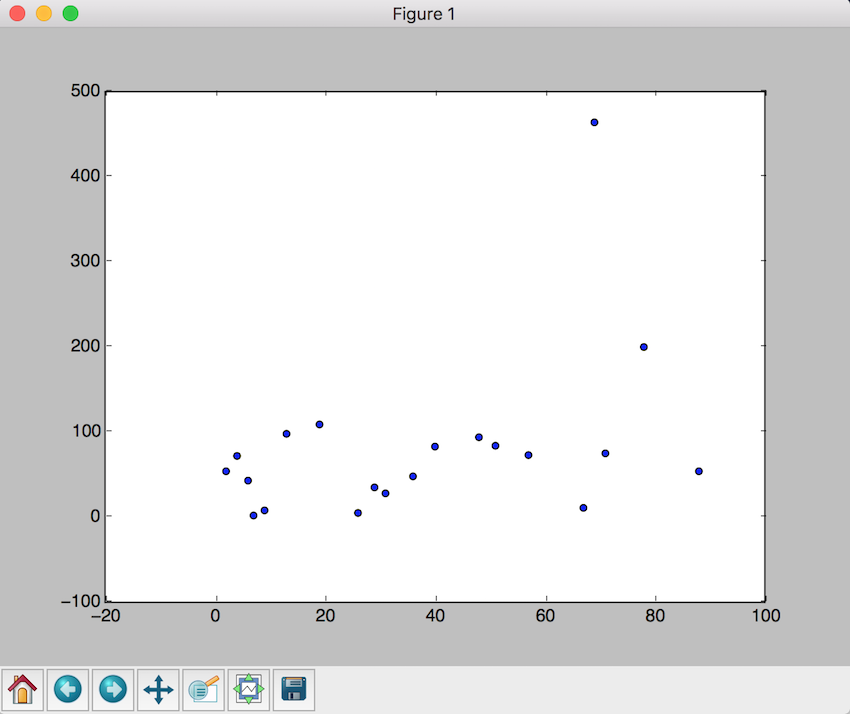
\includegraphics[width=0.85\textwidth]{figures/6/plotsebaran.PNG}}
	\caption{Tampilan Plot Sebaran}
	\label{fig:plotsebaran}
\end{figure}

Tentu saja, kita dapat mengubah warna marker sebagai tambahan untuk pengaturan lainnya, seperti yang ditunjukkan di dalam dokumentasi.

\subsection{Histogram}
Plot histogram adalah sebuah grafik yang menampilkan frekuensi data menggunakan sebuah batang, dimana angka dikelompokkan dalam rentang yang tertentu. Dengan kata lain, frekuensi setiap elemen data di dalam daftar ditunjukkan menggunakan histogram. Angka yang dikelompokkan dalam bentuk rentang tertentu. Mari lihat contoh untuk lebih mengerti ini.

Contoh data yang ingin kita tentukan histogramnya adalah sebagai berikut:
\begin{verbatim}
x = [2,4,6,5,42,543,5,3,73,64,43,97,63,76,63,8,73,97,23,45,56,89,45,3,23,2,5,78,23,56,67,78,8,3,78,34,67,23,324,234,43,544,54,33,223,443,444,234,76,432,233,23,232,242,222,221,254,222,276,300,353,354,387,364,398]
\end{verbatim}
Script Python yang dapat kita gunakan untuk menampilkan histogram seperti pada listing \ref{lst:histogram} : 
\lstinputlisting[caption=Skrip Histogram, label={lst:histogram}]{src/6/histogram.py}

Ketika kamu menjalankan script, kamu harusnya mendapatkan sesuatu serupa dengan grafik berikut (histogram) seperti pada gambar \ref{fig:histogram}:
\begin{figure}[!htbp]
	\centerline{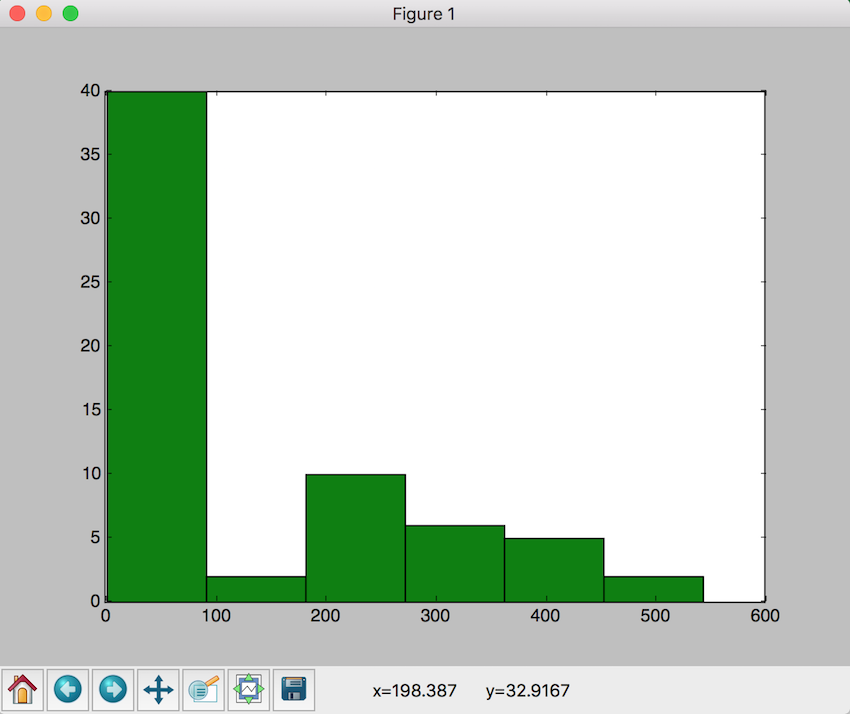
\includegraphics[width=0.85\textwidth]{figures/6/histogram.PNG}}
	\caption{Tampilan Histogram}
	\label{fig:histogram}
\end{figure}

Tentu saja ada lebih banyak parameter untuk function hist, seperti yang ditunjukkan di dokumentasi.

\subsection{Kustomisasi Plot} 
Sekarang kita dapat menambahkan judul, label untuk garis horisontal dan vertikal dengan memanggil fungsi xtitle, xlabel, dan ylabel seperti pada seperti pada listing \ref{lst:cusplot} : 
\lstinputlisting[caption=Skrip Kustomisasi Plot, label={lst:cusplot}]{src/6/cusplot.py}
Seperti pada gambar \ref{fig:cusplot}:
\begin{figure}[!htbp]
	\centerline{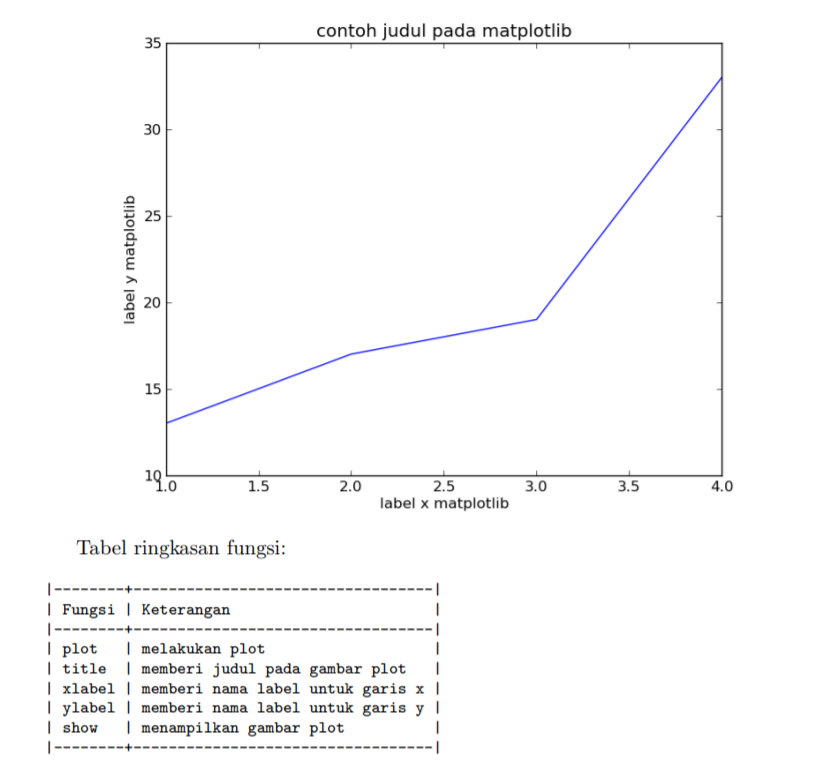
\includegraphics[width=0.85\textwidth]{figures/6/cusplot.PNG}}
	\caption{Tampilan Kustomisasi Plot}
	\label{fig:cusplot}
\end{figure}

\section{Pembacaan data dari sebuah file.txt} 
\subsection{Membuat/memasukkan data melalui notepad}
Cara yang pertama ialah dengan memasukkan seluruh data berupa angka ke sebuah halaman notepad dan kemudian disimpan sebagai file.txt (disini saya membuat nama file hasil.txt)
Seperti pada gambar \ref{fig:hasiltxt}:
\begin{figure}[!htbp]
	\centerline{\includegraphics[width=0.85\textwidth]{figures/6/hasiltxt.PNG}}
	\caption{Data Hasil.txt}
	\label{fig:hasiltxt}
\end{figure}

\subsection{Pembacaan data}
Setelah kita berhasil membuat file dengan nama hasil.txt, kemudian kita akan memanggil file tersebut kesebuah kode program, sehingga source code seperti pada listing \ref{lst:rdata} : 
\lstinputlisting[caption=Skrip Pembacaan Data, label={lst:rdata}]{src/6/rdata.py}

Source code diatas bernama ‘ bacadata.py ‘ lalu dengan menggunakan python kita akan memanggil bacadata.py tersebut. 

Cara pemanggilan sebuah file python adalah sebagai berikut : 
\begin{enumerate}
\item Buka CMD
\item Arahkan ke direktori tempat penyimpanan file python yang kamu buat (disini saya meletakkan file python bacadata.py tersebut di desktop
\item Lalu panggil dengan perintah seperti pada gambar \ref{fig:bacadata}:
\begin{figure}[!htbp]
	\centerline{\includegraphics[width=0.85\textwidth]{figures/6/bacadata.PNG}}
	\caption{Pemanggilan bacadata.py}
	\label{fig:bacadata}
\end{figure}

\item Perlu diketahui bahwa file hasil.txt harus terletak di direktori dan folder yang sama (disini saya meletakkan hasil.txt di dekstop juga)
\item Sehingga jika python bacadata.py maka akan membaca keseluruhan isi angka pada data hasil.txt tersebut.
\item Perlu diketahui lagi bahwa ini hanya membaca dan menampilkan data berupa angka juga, sehingga hasilnya akan seperti gambar diatas.
\end{enumerate}
 
\subsection{Pemanggilan data ke sebuah plot}
Seperti pada listing \ref{lst:dataplot} : 
\lstinputlisting[caption=Skrip Pemanggilan data ke sebuah plot, label={lst:dataplot}]{src/6/dataplot.py}

Dengan menggunakan source code diatas kita bisa memanggil hasil.txt yang telah kita buat tadi ke sebuah fungsi plot, sehingga kita tidak perlu lagi menulis seluruh isi data angka di source code plot, cukup menggunakan ‘with open’ kita dapat memanggil file yang kemudian akan di baca dan ditampilkan berupa plot.

Disini saya membuat file python yang bernama panggildata.py .Sehingga jika kita panggil melalui CMD akan seperti pada gambar \ref{fig:panggildata}:
\begin{figure}[!htbp]
	\centerline{\includegraphics[width=0.85\textwidth]{figures/6/panggildata.PNG}}
	\caption{Pemanggilan panggildata.py}
	\label{fig:panggildata}
\end{figure}

Jika sudah kita panggil maka secara otomatis akan muncul figure baru seperti pada gambar \ref{fig:pplot}:
\begin{figure}[!htbp]
	\centerline{\includegraphics[width=0.85\textwidth]{figures/6/pplot.PNG}}
	\caption{Tampilan pemanggilan data ke sebuah plot}
	\label{fig:pplot}
\end{figure} 

\section{Modifikasi Hasil Plot} 
\subsection{Setting Label} 
Kita dapat Kustomisasi Tampilan pada plot, pertama kita akan membahas tentang label. Anda dapat menambahkan judul, label untuk garis horisontal dan vertikal dengan menambahkan nama label untuk garis x dan y
Disini ada contoh source code untuk menambahkan nama pada label, Seperti pada listing \ref{lst:setlabel} : 
\lstinputlisting[caption=Skrip Setting Label, label={lst:setlabel}]{src/6/setlabel.py}

Adapun hasil yang ditampilkan pada source code diatas adalah seperti pada gambar \ref{fig:setlabel}:
\begin{figure}[!htbp]
	\centerline{\includegraphics[width=0.85\textwidth]{figures/6/setlabel.PNG}}
	\caption{Tampilan setting label}
	\label{fig:setlabel}
\end{figure} 

Pada gambar \ref{fig:setlabel} adalah sebuat plot dengan menambahkan nama pada label x yaitu banyak data dan label y yaitu gelombang otak.

\subsection{Setting Warna}
Selanjutnya kita akan membahas bagaimana kustomisasi warna pada plot, dengan menggunakan facecolor = ‘red’ kita akan menggangi warna plot menjadi merah.

Disini ada contoh source code untuk mengganti warna pada plot, tetapi disini saya coba menggunakan plt.hist, Seperti pada listing \ref{lst:setwarna} : 
\lstinputlisting[caption=Skrip Setting Warna, label={lst:setwarna}]{src/6/setwarna.py}

Jika anda membuat source seperti diatas maka akan menampilkan hasil  seperti pada gambar \ref{fig:setwarna}:
\begin{figure}[!htbp]
	\centerline{\includegraphics[width=0.85\textwidth]{figures/6/setwarna.PNG}}
	\caption{Tampilan setting warna}
	\label{fig:setwarna}
\end{figure} 

Dengan menggunakan perintah facecolor maka kita bisa mengganti warna pada plot dengan warna yang kita inginkan.

\subsection{Setting Marker}
Selanjutnya kita akan kustomisasi marker pada plot, disini kita bisa mengganti penanda label pada x dan y
Ikuti contoh source code Seperti pada listing \ref{lst:swmarker} : 
\lstinputlisting[caption=Skrip Setting Tanpa Marker, label={lst:swmarker}]{src/6/swmarker.py}

Pada source code diatas belum ada kustomisasi marker yang dibuat, lalu  hasilnya akan seperti pada gambar \ref{fig:swmarker}:
\begin{figure}[!htbp]
	\centerline{\includegraphics[width=0.85\textwidth]{figures/6/swmarker.PNG}}
	\caption{Tampilan setting tanpa marker}
	\label{fig:swmarker}
\end{figure} 

Sekarang coba kita bandingkan dengan source code berikut yang ditambahkan marker untuk kustomisasi penanda label x Seperti pada listing \ref{lst:setmarker} : 
\lstinputlisting[caption=Skrip Setting Dengan Marker, label={lst:setmarker}]{src/6/setmarker.py}
dan hasilnya akan seperti pada gambar \ref{fig:setmarker}:
\begin{figure}[!htbp]
	\centerline{\includegraphics[width=0.85\textwidth]{figures/6/setmarker.PNG}}
	\caption{Tampilan setting dengan marker}
	\label{fig:setmarker}
\end{figure} 

Berbeda bukan sama yang gambar sebelumnya ? nah itu bisa kita kustomisasi dengan menambahkan marker pada plt.plot(x, marker='o') bisa juga o diganti dengan x dan sebagainya.

\subsection{Jenis Plot}
Pada pembahasan diawal sudah kita bahas tentang dasar-dasar plot, disini akan kita berikan hasil tampilkan pada jenis-jenis plot yang ada [4].
\begin{enumerate}
\item Plot Garis, seperti pada gambar \ref{fig:pltgaris}:
\begin{figure}[!htbp]
	\centerline{\includegraphics[width=0.85\textwidth]{figures/6/pltgaris.PNG}}
	\caption{Tampilan jenis plot garis}
	\label{fig:pltgaris}
\end{figure} 

\item Plot Sebaran, seperti pada gambar \ref{fig:pltsebaran}:
\begin{figure}[!htbp]
	\centerline{\includegraphics[width=0.85\textwidth]{figures/6/pltsebaran.PNG}}
	\caption{Tampilan jenis plot sebaran}
	\label{fig:pltsebaran}
\end{figure}

\item Histogram, seperti pada gambar \ref{fig:histogrm}:
\begin{figure}[!htbp]
	\centerline{\includegraphics[width=0.85\textwidth]{figures/6/histogrm.PNG}}
	\caption{Tampilan jenis plot histogram}
	\label{fig:histogrm}
\end{figure}

\item Bar Charts, seperti pada gambar \ref{fig:barchart}:
\begin{figure}[!htbp]
	\centerline{\includegraphics[width=0.85\textwidth]{figures/6/barchart.PNG}}
	\caption{Tampilan jenis plot bar charts}
	\label{fig:barchart}
\end{figure}

\item Pie, seperti pada gambar \ref{fig:pltpie}:
\begin{figure}[!htbp]
	\centerline{\includegraphics[width=0.85\textwidth]{figures/6/pltpie.PNG}}
	\caption{Tampilan jenis plot pie}
	\label{fig:pltpie}
\end{figure}

\item Hist, seperti pada gambar \ref{fig:hist}:
\begin{figure}[!htbp]
	\centerline{\includegraphics[width=0.85\textwidth]{figures/6/hist.PNG}}
	\caption{Tampilan jenis plot hist}
	\label{fig:hist}
\end{figure}

\item 3D Line, seperti pada gambar \ref{fig:3dline}:
\begin{figure}[!htbp]
	\centerline{\includegraphics[width=0.85\textwidth]{figures/6/3dline.PNG}}
	\caption{Tampilan jenis plot 3D Line}
	\label{fig:3dline}
\end{figure}

\item 3D Scatter Plot, seperti pada gambar \ref{fig:3dscatter}:
\begin{figure}[!htbp]
	\centerline{\includegraphics[width=0.85\textwidth]{figures/6/3dscatter.PNG}}
	\caption{Tampilan jenis plot 3D Scatter}
	\label{fig:3dscatter}
\end{figure}

\item 3D Bar Charts, seperti pada gambar \ref{fig:3dchart}:
\begin{figure}[!htbp]
	\centerline{\includegraphics[width=0.85\textwidth]{figures/6/3dchart.PNG}}
	\caption{Tampilan jenis plot 3D Charts}
	\label{fig:3dchart}
\end{figure}
\end{enumerate}

\section{Plot Ditampilkan Dan Disimpan}
Sekarang kita akan membahas bagaimana cara untuk membuat plot itu bisa disimpan sebagai gambar tanpa kita panggil melalui python.
\subsection{Plot Ditampilkan}
Seperti tutorial yang sebelumnya bagaimana kita sudah mempelajari bagaimana menampilkan data menjadi sebuah plot, kita ulas kembali bagaimana caranya, dengan memanfaatkan script diawal tadi Seperti pada listing \ref{lst:showplt} : 
\lstinputlisting[caption=Skrip Plot ditampilkan, label={lst:showplt}]{src/6/showplt.py}
Hasilnya juga akan sama seperti tutorial diawal tadi seperti pada gambar \ref{fig:hasilplot}:
\begin{figure}[!htbp]
	\centerline{\includegraphics[width=0.85\textwidth]{figures/6/hasilplot.PNG}}
	\caption{Hasil plot ditampilkan}
	\label{fig:hasilplot}
\end{figure} 

\subsection{Plot Disimpan}
Sekarang kita akan membahas bagaimana suatu data yang sudah kita transformasi menjadi sebuah plot bisa tersimpan sebagai gambar. 
Script sama seperti Tabel 6.10 tadi, disini kita fokus ke hasil pada Gambar 6.21, ada sebuah menu dibawah hasil yang ditampilkan. 
Perhatikan gambar  \ref{fig:menuplot}:
\begin{figure}[!htbp]
	\centerline{\includegraphics[width=0.85\textwidth]{figures/6/menuplot.PNG}}
	\caption{Menu plot disimpan}
	\label{fig:menuplot}
\end{figure} 

Dengan memanfaatkan menu save yang ada pada tampilan diatas maka secara otomatis kita bisa menyimpan hasil plot menjadi gambar ke lokasi file yang kita mau seperti pada gambar \ref{fig:prosesplot}:
\begin{figure}[!htbp]
	\centerline{\includegraphics[width=0.85\textwidth]{figures/6/prosesplot.PNG}}
	\caption{Proses plot disimpan}
	\label{fig:prosesplot}
\end{figure} 

\section{Penanganan Error Pada Pemasangan Matlotlib}
Disini saya menggunakan sistem operasi windows, sebelum anda menginstall matplotlib kita harus memasang python terlebih dahulu. Disini saya menggunakan python 2,7.

Langsung saja kita pergi ke CMD lalu ketikan pip install matplotlib seperti pada gambar \ref{fig:errormat}:
\begin{figure}[!htbp]
	\centerline{\includegraphics[width=0.85\textwidth]{figures/6/errormat.PNG}}
	\caption{Error Pemasangan Matplotlib}
	\label{fig:errormat}
\end{figure} 

Gambar \ref{fig:errormat} adalah tampilan error pada saat kita install matplotlib, coba anda teliti dimanakah letak error tersebut ? 
Error terletak pada sintaks ‘pip instal matplotlib‘ yang seharunya ‘pip install matplotlib’ tampaknya hanya hal kecil tapi dengan kita salah membuat sintaks maka hasil juga akan error sehingga perintah yang benar seperti pada gambar \ref{fig:pasangmat}:
\begin{figure}[!htbp]
	\centerline{\includegraphics[width=0.85\textwidth]{figures/6/pasangmat.PNG}}
	\caption{Pemasangan Matplotlib}
	\label{fig:pasangmat}
\end{figure} 

Jika tampilan sudah seperti gambar \ref{fig:pasangmat}, maka matplotlib telah terpasang dan siap digunakan [2].

\section{Error Pada Saat Menggambar Plot Dasar}
Sekarang kita akan membahas tentang membuat sebuah plot dasar, atau membaca sebuah data yang berupa angka menjadi sebuah plot.
\subsection{Error Pada Plot Garis}
Kita akan membahas sebuah contoh sederhana dalam menggambar sebuah plot garis menggunakan matplotlib. Dalam contoh ini, kita akan membuat sebuah garis dari data angka yang memiliki sumbu x dan y.
Untuk data yang akan kita buat sebagai plot adalah sebagai berikut : 
\begin{verbatim}
x = (4,8,13,17,20)
y = (54, 67, 98, 78, 45)
\end{verbatim}
Ini dapat dilakukan dengan menggunakan script Seperti pada listing \ref{lst:pltgaris} : 
\lstinputlisting[caption=Skrip Plot Garis, label={lst:pltgaris}]{src/6/pltgaris.py}
seperti pada gambar \ref{fig:errpltgaris}:
\begin{figure}[!htbp]
	\centerline{\includegraphics[width=0.85\textwidth]{figures/6/errpltgaris.PNG}}
	\caption{Skrip Error Plot Garis}
	\label{fig:errpltgaris}
\end{figure}

seperti pada gambar \ref{fig:errpltgrs}:
\begin{figure}[!htbp]
	\centerline{\includegraphics[width=0.85\textwidth]{figures/6/errpltgrs.PNG}}
	\caption{Error Plot Garis}
	\label{fig:errpltgrs}
\end{figure}            

Pada contoh di atas saya membuat file dengan nama test.py, dan saya panggil melalui python. Sintaks diatas adalah error karena plt.show() tidak sejajar dengan baris kedua sehingga di baca oleh program plt.show() itu adalah turunan dari baris kedua, sehingga solusinya seperti pada gambar \ref{fig:solepg}:
\begin{figure}[!htbp]
	\centerline{\includegraphics[width=0.85\textwidth]{figures/6/solepg.PNG}}
	\caption{Solusi Error Plot Garis}
	\label{fig:solepg}
\end{figure}            

Dan jika dipanggil melalui python hasilnya akan seperti pada gambar \ref{fig:erpg}:
\begin{figure}[!htbp]
	\centerline{\includegraphics[width=0.85\textwidth]{figures/6/erpg.PNG}}
	\caption{Error Plot Garis}
	\label{fig:erpg}
\end{figure}       

Gambar \ref{fig:erpg} adalah error kedua pada program plot garis, disini errornya adalah kita tidak meletakkan koma di antara sumbu x dan y, bisa kita temui di 
plt.plot([4,8,13,17,20] [54, 67, 98, 78, 45]) yang seharusnya seperti pada gambar \ref{fig:solpg}:
\begin{figure}[!htbp]
	\centerline{\includegraphics[width=0.85\textwidth]{figures/6/solpg.PNG}}
	\caption{Solusi Error Plot Garis}
	\label{fig:solpg}
\end{figure}       

\subsection{Plot Sebaran}
Sebuah plot sebaran adalah sebuah grafik yang menunjukkan hubungan antara dua set data, di plot sebaran ini digambarkan melalui titik titik yang saling terhubung ke angka-angka yang ada di sumbu x dan y. Di dalam contoh ini, kita akan membahas menggambar sebuah plot sebaran menggunakan matplotlib.

Untuk data yang akan kita buat sebagai plot adalah sebagai berikut : 
\begin{verbatim}
x = [2,4,6,7,9,13,19,26,29,31,36,40,48,51,57,67,69,71,78,88]
y = [54,72,43,2,8,98,109,5,35,28,48,83,94,84,73,11,464,75,200,54]
\end{verbatim}
Plot sebaran dapat digambarkan menggunakan script Seperti pada listing \ref{lst:pltsebaran} : 
\lstinputlisting[caption=Skrip Plot Sebaran, label={lst:pltsebaran}]{src/6/pltsebaran.py}

Masalah atau error yang biasa timbul adalah seperti pada gambar \ref{fig:errpltsebaran}:
\begin{figure}[!htbp]
	\centerline{\includegraphics[width=0.85\textwidth]{figures/6/errpltsebaran.PNG}}
	\caption{Error Plot Sebaran}
	\label{fig:errpltsebaran}
\end{figure}       

Solusinya adalah dengan menambahkan koma di antara x dan y (x,y)
Atau seperti pada gambar \ref{fig:soleps}:
\begin{figure}[!htbp]
	\centerline{\includegraphics[width=0.85\textwidth]{figures/6/soleps.PNG}}
	\caption{Solusi Error Plot Sebaran}
	\label{fig:soleps}
\end{figure}      

Dalam contoh lain error bisa menjadi seperti pada gambar \ref{fig:errpltseb}:
\begin{figure}[!htbp]
	\centerline{\includegraphics[width=0.85\textwidth]{figures/6/errpltseb.PNG}}
	\caption{Error Plot Sebaran}
	\label{fig:errpltseb}
\end{figure}       

Solusinya adalah terdapat pada plt.scatter(y) yang seharunya menjadi  plt.scatter(x,y) karena tidak mungkin kita mau menampilkan gambar yang sudah kita defenisikan x dan y tetapi kita hanya menampilkan 1 sumbu saja,
Dalam contoh ini, hasilnya akan menjadi seperti pada gambar \ref{fig:solepsb}:
\begin{figure}[!htbp]
	\centerline{\includegraphics[width=0.85\textwidth]{figures/6/solepsb.PNG}}
	\caption{Solusi Error Plot Sebaran}
	\label{fig:solepsb}
\end{figure}      

\subsection{Error Pada Histogram}
Plot histogram adalah sebuah grafik yang menampilkan frekuensi data menggunakan sebuah batang, dimana angka dikelompokkan dalam rentang yang tertentu. Dengan kata lain, frekuensi setiap elemen data di dalam daftar ditunjukkan menggunakan histogram. Angka yang dikelompokkan dalam bentuk rentang tertentu. Mari lihat contoh untuk lebih mengerti ini.
Contoh data yang ingin kita tentukan histogramnya adalah sebagai berikut:
\verb|x = [2,4,6,5,42,543,5,3,73,64,43,97,63,76,63,8,73,97,23,45,56,89,45,3,23,2,5,78,23,56,67,78,8,3,78,34,67,23,324,234,43,544,54,33,223,443,444,234,76,432,233,23,232,242,222,221,254,222,276,300,353,354,387,364,398]|
Script Python yang dapat kita gunakan untuk menampilkan histogram pada data di atas adalah Seperti pada listing \ref{lst:histogrm} : 
\lstinputlisting[caption=Skrip Histogram, label={lst:histogrm}]{src/6/histogrm.py}

Error yang biasa ditemukan adalah seperti pada gambar \ref{fig:errhisto}:
\begin{figure}[!htbp]
	\centerline{\includegraphics[width=0.85\textwidth]{figures/6/errhisto.PNG}}
	\caption{Error Histogram}
	\label{fig:errhisto}
\end{figure}       

Solusi untuk error diatas adalah pada saat mengetik script ada yang terlewat tanpa memberikan koma setelah angka, disini kita lupa memberi koma pada 97 dan 63. Seharusnya seperti pada gambar \ref{fig:solhisto}:
\begin{figure}[!htbp]
	\centerline{\includegraphics[width=0.85\textwidth]{figures/6/solhisto.PNG}}
	\caption{Solusi Error Histogram}
	\label{fig:solhisto}
\end{figure}      

Kalau dari error yanglain adalah kita sebagai orang indonesia yang masih awam dengan sebutan warna atau color untuk program, tanpa sengaja kita mendefenisikan color=hijau. Itu jelas salah karena komputer atau program tidak akan mengerti bahasa itu, disini dapat kita ubah dengan facecolor = ‘green’ atau seperti pada gambar \ref{fig:solhistogrm}:
\begin{figure}[!htbp]
	\centerline{\includegraphics[width=0.85\textwidth]{figures/6/solhistogrm.PNG}}
	\caption{Solusi Error Histogram}
	\label{fig:solhistogrm}
\end{figure}      

Hasil tampilannya seperti pada gambar \ref{fig:showhisto}:
\begin{figure}[!htbp]
	\centerline{\includegraphics[width=0.85\textwidth]{figures/6/showhisto.PNG}}
	\caption{Tampilan Histogram}
	\label{fig:showhisto}
\end{figure} 

\subsection{Error Pada Saat Kustomisasi Plot} 
Sekarang kita dapat menambahkan judul, label untuk garis horisontal dan vertikal dengan memanggil fungsi xtitle, xlabel, dan ylabel Seperti pada listing \ref{lst:cuserrplt} : 
\lstinputlisting[caption=Kustomisasi Plot, label={lst:cuserrplt}]{src/6/cuserrplt.py}
Pada script diatas sudah ada fungsi title, xlabel dan ylabel.Tetapi ada beberapa error yang mungkin didapat jika kita salah pada pengetikan, seperti pada gambar \ref{fig:errcusplot}:
\begin{figure}[!htbp]
	\centerline{\includegraphics[width=0.85\textwidth]{figures/6/errcusplot.PNG}}
	\caption{Error Kustomisasi Plot}
	\label{fig:errcusplot}
\end{figure}       

Solusi dari error diatas adalah dengan menambahkan tanda kutip pada setiap kita mendefenisikan title, sehingga seperti pada gambar \ref{fig:solcusplot}:
\begin{figure}[!htbp]
	\centerline{\includegraphics[width=0.85\textwidth]{figures/6/solcusplot.PNG}}
	\caption{Solusi Error Kustomisasi Plot}
	\label{fig:solcusplot}
\end{figure}      

seperti pada gambar \ref{fig:errcusplt}:
\begin{figure}[!htbp]
	\centerline{\includegraphics[width=0.85\textwidth]{figures/6/errcusplt.PNG}}
	\caption{Error Kustomisasi Plot}
	\label{fig:errcusplt}
\end{figure}
Error \ref{fig:errcusplt} adalah kesalahan penulisan pada fungsi plt.tittle yang seharusnya digunakan plt.title (tanpa double T) atau seperti pada gambar \ref{fig:solcp}:
\begin{figure}[!htbp]
	\centerline{\includegraphics[width=0.85\textwidth]{figures/6/solcp.PNG}}
	\caption{Solusi Error Kustomisasi Plot}
	\label{fig:solcp}
\end{figure}

Hasil tampilannya seperti pada gambar \ref{fig:showcp}:
\begin{figure}[!htbp]
	\centerline{\includegraphics[width=0.85\textwidth]{figures/6/showcp.PNG}}
	\caption{Tampilan Kustomisasi Plot}
	\label{fig:showcp}
\end{figure} 

\section{Error Pada Pembacaan data dari sebuah file.txt} 
\subsection{Membuat/memasukkan data melalui notepad}
Cara yang pertama ialah dengan memasukkan seluruh data berupa angka ke sebuah halaman notepad dan kemudian disimpan sebagai file.txt (disini saya membuat nama file hasil.txt) seperti pada gambar \ref{fig:datahasil}:
\begin{figure}[!htbp]
	\centerline{\includegraphics[width=0.85\textwidth]{figures/6/datahasil.PNG}}
	\caption{Data Hasil.txt}
	\label{fig:datahasil}
\end{figure} 

\subsection{Error Pada Pembacaan data}
Setelah kita berhasil membuat file dengan nama hasil.txt, kemudian kita akan memanggil file tersebut kesebuah kode program, sehingga source code akan Seperti pada listing \ref{lst:rdt} : 
\lstinputlisting[caption=Skrip Pembacaan data, label={lst:rdt}]{src/6/rdt.py}

Source code diatas bernama ‘ bacadata.py ‘ lalu dengan menggunakan python kita akan memanggil bacadata.py tersebut. 
Cara pemanggilan sebuah file python adalah sebagai berikut :
\begin{enumerate} 
\item Buka CMD
\item Arahkan ke direktori tempat penyimpanan file python yang kamu buat (disini saya meletakkan file python bacadata.py tersebut di desktop
\item Lalu panggil dengan perintah berikut seperti pada gambar \ref{fig:panggilbcdt}:
\begin{figure}[!htbp]
	\centerline{\includegraphics[width=0.85\textwidth]{figures/6/panggilbcdt.PNG}}
	\caption{Panggil File bacadata.py}
	\label{fig:panggilbcdt}
\end{figure} 
Adapun error-error pada script diatas ialah seperti pada gambar \ref{fig:errdata}:
\begin{figure}[!htbp]
	\centerline{\includegraphics[width=0.85\textwidth]{figures/6/errdata.PNG}}
	\caption{Error pada pembacaan data}
	\label{fig:errdata}
\end{figure} 

Error diatas didapatkan dari script dibawah ini  seperti pada gambar \ref{fig:lsterrdata}:
\begin{figure}[!htbp]
	\centerline{\includegraphics[width=0.85\textwidth]{figures/6/lsterrdata.PNG}}
	\caption{Script Error pada pembacaan data}
	\label{fig:lsterrdata}
\end{figure} 

Yang membedakan script diatas dengan script diawal iyalah kita secara tidak sengaja lupa memberi kurung penutup pada script diatas, sehingga solusinya ialah seperti pada gambar \ref{fig:solerrdata}:
\begin{figure}[!htbp]
	\centerline{\includegraphics[width=0.85\textwidth]{figures/6/solerrdata.PNG}}
	\caption{Solusi Error pada pembacaan data}
	\label{fig:solerrdata}
\end{figure} 

Adapun hasil dari script pada pembacaan data diatas ialah seperti pada gambar \ref{fig:showdata}:
\begin{figure}[!htbp]
	\centerline{\includegraphics[width=0.85\textwidth]{figures/6/showdata.PNG}}
	\caption{Tampilan pada pembacaan data}
	\label{fig:showdata}
\end{figure} 
\end{enumerate}

\subsection{Error Pemanggilan data ke sebuah plot}
Seperti pada listing \ref{lst:panggildp} : 
\lstinputlisting[caption=Skrip pemanggilan data ke sebuah plot, label={lst:rdt}]{src/6/panggildp.py}

Pada script diatas kita akan memanggil atau membaca file yang telah kita buat tadi yang bernama hasil.txt, tetapi biasa terdapat error-error pada script tersebut yaitu seperti pada gambar \ref{fig:errpd}:
\begin{figure}[!htbp]
	\centerline{\includegraphics[width=0.85\textwidth]{figures/6/errpd.PNG}}
	\caption{Error pemanggilan data}
	\label{fig:errpd}
\end{figure} 

Error pada gambar diatas terdapat pada x.append(int(row[1])) disini artinya kita membaca data pada baris kedua, jika [0] maka baris pertama dan [2] maka baris kedua dan seterusnya. Itulah yang menyebabkan script bisa jadi error, sehingga solusi nya adalah mengganti angka 1 dengan 0 seperti pada gambar \ref{fig:solepd}:
\begin{figure}[!htbp]
	\centerline{\includegraphics[width=0.85\textwidth]{figures/6/solepd.PNG}}
	\caption{Solusi Error pemanggilan data}
	\label{fig:solepd}
\end{figure} 

Error lainnya seperti pada gambar \ref{fig:epd}:
\begin{figure}[!htbp]
	\centerline{\includegraphics[width=0.85\textwidth]{figures/6/epd.PNG}}
	\caption{Error pemanggilan data}
	\label{fig:epd}
\end{figure} 

Pada gambar diatas coba kita teliti kembali pada script yang diawal,  for row in plots, seharusnya setelah itu kita tambahkan ‘:’ agar tidak error seperti pada gambar \ref{fig:sepd}:
\begin{figure}[!htbp]
	\centerline{\includegraphics[width=0.85\textwidth]{figures/6/sepd.PNG}}
	\caption{Solusi Error pemanggilan data}
	\label{fig:sepd}
\end{figure} 
  
Error lainnya seperti pada gambar \ref{fig:etpd}:
\begin{figure}[!htbp]
	\centerline{\includegraphics[width=0.85\textwidth]{figures/6/etpd.PNG}}
	\caption{Error tampilan  pemanggilan data}
	\label{fig:etpd}
\end{figure} 

Pada gambar diatas didapatkan dari script berikut Seperti pada listing \ref{lst:etpd} : 
\lstinputlisting[caption=Contoh Skrip error pemanggilan data ke sebuah plot, label={lst:etpd}]{src/6/etpd.py}

Namun kenapa masih kosong tanpa ada gambaran sebuah plot ? Itu karena kita tidak meletakkan sumbu yang ingin dibaca oleh program, yaitu sumbu x, error terdapat pada baris ke 13, yang seharusnya seperti pada gambar \ref{fig:solerrpd}:
\begin{figure}[!htbp]
	\centerline{\includegraphics[width=0.85\textwidth]{figures/6/solerrpd.PNG}}
	\caption{Solusi Error pemanggilan data}
	\label{fig:solerrpd}
\end{figure} 

Error lainnya seperti pada gambar \ref{fig:errpdl}:
\begin{figure}[!htbp]
	\centerline{\includegraphics[width=0.85\textwidth]{figures/6/errpdl.PNG}}
	\caption{Error pemanggilan data}
	\label{fig:errpdl}
\end{figure} 

Adapun error diatas karena kita mengganti marker menjadi A dan tidak bisa di pahami oleh program,adapun marker yang bisa kita buat pada matplotlib yaitu seperti pada gambar \ref{fig:markermat}:
\begin{figure}[!htbp]
	\centerline{\includegraphics[width=0.85\textwidth]{figures/6/markermat.PNG}}
	\caption{Marker Pada Matplotlib}
	\label{fig:markermat}
\end{figure} 

Sekarang contoh jika kita ingin mengubah marker menjadi square yaitu seperti pada gambar \ref{fig:lstmar}:
\begin{figure}[!htbp]
	\centerline{\includegraphics[width=0.85\textwidth]{figures/6/lstmar.PNG}}
	\caption{Skrip Marker Pada Matplotlib}
	\label{fig:lstmar}
\end{figure} 

Adapun hasil dari script diatas jika mengubah marker menjadi s ialah seperti pada gambar \ref{fig:solem}:
\begin{figure}[!htbp]
	\centerline{\includegraphics[width=0.85\textwidth]{figures/6/solem.PNG}}
	\caption{Solusi Error Marker}
	\label{fig:solem}
\end{figure}  

\section{Error Pada Modifikasi Hasil Plot}
\subsection{Error Setting Label} 
Kita dapat Kustomisasi Tampilan pada plot, pertama kita akan membahas tentang label. Anda dapat menambahkan judul, label untuk garis horisontal dan vertikal dengan menambahkan nama label untuk garis x dan y
Disini ada contoh source code untuk menambahkan nama pada label, Seperti pada listing \ref{lst:settlbl} : 
\lstinputlisting[caption=Skrip Setting Label, label={lst:settlbl}]{src/6/settlbl.py}

Pada script diatas kita dapat mengubah kalimat yang terdapat pada xlabel dan ylabel. 
Tetapi setidaknya ada beberapa error yang biasa dialami pada script diatas yaitu seperti pada gambar \ref{fig:errsetlbl}:
\begin{figure}[!htbp]
	\centerline{\includegraphics[width=0.85\textwidth]{figures/6/errsetlbl.PNG}}
	\caption{Error Setting Label}
	\label{fig:errsetlbl}
\end{figure}  

Seperti yang error sebelumnya juga, kita secara tidak sengaja lupa memberi tanda kutip pada xlabel dan ylabel sehingga solusinya adalah seperti pada gambar \ref{fig:solesl}:
\begin{figure}[!htbp]
	\centerline{\includegraphics[width=0.85\textwidth]{figures/6/solesl.PNG}}
	\caption{Solusi Error Setting Label}
	\label{fig:solesl}
\end{figure}  

Adapun hasil dari setting label adalah seperti pada gambar \ref{fig:showtsesl}:
\begin{figure}[!htbp]
	\centerline{\includegraphics[width=0.85\textwidth]{figures/6/showtsesl.PNG}}
	\caption{Tampilan Solusi Error Setting Label}
	\label{fig:showtsesl}
\end{figure}   
Yang bertanda merah ialah xlabel dan ylabel yang telahdi setting

Adapun hasil yang ditampilkan pada source code diatas adalah seperti pada gambar \ref{fig:showsl}:
\begin{figure}[!htbp]
	\centerline{\includegraphics[width=0.85\textwidth]{figures/6/showsl.PNG}}
	\caption{Tampilan Setting Label}
	\label{fig:showsl}
\end{figure}   

\subsection{Error Setting Warna}
Selanjutnya kita akan membahas bagaimana kustomisasi warna pada plot, dengan menggunakan facecolor = ‘red’ kita akan menggangi warna plot menjadi merah.

Disini ada contoh source code untuk mengganti warna pada plot, tetapi disini saya coba menggunakan plt.hist, Seperti pada listing \ref{lst:settwarna} : 
\lstinputlisting[caption=Skrip setting warna, label={lst:settwarna}]{src/6/settwarna.py}

Pada script diatas kita akan mengubah color atau warna pada plot hist yang akan kita baca dari data hasil.txt, tetapi ada beberapa error yang di dapat sebelum script diatas dibuat seperti pada gambar \ref{fig:errsetwar}:
\begin{figure}[!htbp]
	\centerline{\includegraphics[width=0.85\textwidth]{figures/6/errsetwar.PNG}}
	\caption{Error Setting Warna}
	\label{fig:errsetwar}
\end{figure}   

Pada gambar diatas kita salah memberikan warna pada facecolor yang scriptnya seperti pada gambar \ref{fig:solesw}:
\begin{figure}[!htbp]
	\centerline{\includegraphics[width=0.85\textwidth]{figures/6/solesw.PNG}}
	\caption{Solusi Error Setting Warna}
	\label{fig:solesw}
\end{figure}   

Python tidak memahami pendefenisian merah untuk facecolor, adapun kurang lebih modul color pada matplotlib adalah seperti pada gambar \ref{fig:wsa}:
\begin{figure}[!htbp]
	\centerline{\includegraphics[width=0.85\textwidth]{figures/6/wti.PNG}}
	\caption{Color Pada Matplotlib 3}
	\label{fig:wti}
\end{figure}   

\begin{figure}[!htbp]
	\centerline{\includegraphics[width=0.85\textwidth]{figures/6/wdu.PNG}}
	\caption{Color Pada Matplotlib 2}
	\label{fig:wdu}
\end{figure}   

\begin{figure}[!htbp]
	\centerline{\includegraphics[width=0.85\textwidth]{figures/6/wsa.PNG}}
	\caption{Color Pada Matplotlib 1}
	\label{fig:wsa}
\end{figure}   

Adapun solusi dari error warna tersebut ialah dengan membuat nama warna sesuai modul yang ada pada matplotlib seperti pada gambar \ref{fig:solwa}:
\begin{figure}[!htbp]
	\centerline{\includegraphics[width=0.85\textwidth]{figures/6/solwa.PNG}}
	\caption{Solusi Error Color Pada Matplotlib}
	\label{fig:solwa}
\end{figure}   

Adapun hasil dari script diatas ialah seperti pada gambar \ref{fig:showclr}:
\begin{figure}[!htbp]
	\centerline{\includegraphics[width=0.85\textwidth]{figures/6/showclr.PNG}}
	\caption{Tampilan Setting Warna}
	\label{fig:showclr}
\end{figure}   

\subsection{Error Pada Setting Marker}
Selanjutnya kita akan kustomisasi marker pada plot, disini kita bisa mengganti penanda label pada x dan y
Ikuti contoh source code berikut Seperti pada listing \ref{lst:setmar} : 
\lstinputlisting[caption=Skrip setting marker, label={lst:setmar}]{src/6/setmar.py}

Error yang paling sering dalam mengganti atau mengubah marker ialah kita tidak memperhatikan besar dan kecilnya huruf pada modul marker tersebut, sehingga jika kita mau membuat marker Square yaitu dengan huruf s (kecil) tetapi di script kita meletakkan S (besar) maka itu akan terjadi error seperti pada gambar \ref{fig:errsw}:
\begin{figure}[!htbp]
	\centerline{\includegraphics[width=0.85\textwidth]{figures/6/errsw.PNG}}
	\caption{Error Setting Marker}
	\label{fig:errsw}
\end{figure}   

Solusinya ialah dengan mengikuti modul matplotlib yang ada dengan mengganti s seperti pada gambar \ref{fig:solsw}:
\begin{figure}[!htbp]
	\centerline{\includegraphics[width=0.85\textwidth]{figures/6/solsw.PNG}}
	\caption{Solusi Setting MArker}
	\label{fig:solsw}
\end{figure}   


             Gambar 6.46 Solusi Error Setting Warna
dan hasilnya akan seperti pada gambar \ref{fig:showsw}:
\begin{figure}[!htbp]
	\centerline{\includegraphics[width=0.85\textwidth]{figures/6/showsw.PNG}}
	\caption{Tampilan Setting Marker}
	\label{fig:showsw}
\end{figure}

\chapter{Pengenalan Flask}
\section{Definisi \textit{Micro Frameworki}}

\textit{Microframework} adalah istilah yang digunakan untuk merujuk pada kerangka kerja web minimalis. Kerangka ini sangat berbeda dengan kerangka kerja tumpukan penuh. Juga tidak memiliki sebagaian besar fungsionalitas yang umum yang ada dalam kerangka kerja aplikasi web lengkap, seperti:
\begin{enumerate}
\item Akun, otentikasi, otorisasi, peran, dll.
\item Abtraksi basis data melalui pemetaan objek-relasional.
\item Validai  \textit{input} dan sanitasi \textit{input}.
\item Mesin \textit{template web}.
\end{enumerate}

Biasanya, sebuah \textit{microframework} memfasilitasi menerima permintaan HTTP, merutekan permintaan HTTP ke \textit{controller} yang sesuai, mengirim \textit{controller}, dan mengembalikan respons HTTP. \textit{Microframeworks} seringkali dirancang khusus untuk membangun API untuk layanan atau aplikasi lain. Misalnya, Lumen \textit{microframework} dirancang untuk pengembangan \textit{Microservices} dan pengembangan API. \textit{Microframework}, sebuah \textit{tool} yang digunakan untuk \textit{project} yang lebih kecil dan penggunaan untuk kasus yang spesifik. Ini sama saja dengan menyederhanakan \textit{framework} agar lebih mudah dalam implementasi dan menyediakan \textit{testing} dan \textit{deployment} yang lebih cepat. \textit{Microframework} mengeluarkan banyak sekali komponen yang ada pada pengaturanan \textit{full-stack}, termasuk:
\begin{enumerate}
\item \textit{Web template engine}
\item \textit{Input validation}
\item \textit{Database abstraction}
\item \textit{Roles, accounts, and authentication}
\end{enumerate}

Kerugian menggunakan  \textit{microframework} adalah saat  \textit{project} mulai tumbuh besar dengan cepat. Dimana  \textit{microframework} tidak memiliki fitur yang dibutuhkan untuk mengakomodasi pertumbuhan  \textit{website}. Dengan kata lain kamu kehilangan fleksibelitas.  \textit{Micro-framework} lebih baik saat digunakan untuk  \textit{project} kecil yang membutuhkan kesederhanaan,  \textit{overhead} yang rendah dan  \textit{deployment} yang cepat.  \textit{Developer} yang sudah berpengalaman bisa saja menggunakan  \textit{microframework} pada awal  \textit{project} dan menambahkan tambahan  \textit{microframework} jika diperlukan. Hal ini merupakan pilihan yang menarik, tetapi untuk pemula dan  \textit{developer} menengah harus menghindari ini \cite{fadhilnet}.

\section{Jenis-Jenis \textit{Framework} Python serta Kelebihan dan Kekurangan}

\subsection{Django}

Django adalah kerangka kerja web Python yang memungkinkan individu dalam pengembangan yang bersih dan cepat. Kerangka kerja web secara umum dikatakan sebagai campuran komponen yang membantu pengembang mengembangkan situs web lebih cepat dan mudah. Karena itu, ini adalah kerangka kerja sumber bebas dan terbuka. Ini dapat disebut sebagai kerangka kerja yang memungkinkan pengembang untuk mengambil konsep penyelesaian secepat mungkin. Django sebagai kerangka kerja membantu mengurangi beberapa kesalahan keamanan umum yang dapat diawasi dengan mudah saat mengembangkan aplikasi. Skalabilitas adalah fitur lain yang disediakan oleh kerangka ini.

Django memiliki \textit{tagline "The web framework for perfectionists with deadlines"}, bagaimana tidak, karena secara \textit{default} Django sudah memiliki berbagai modul umum yang biasa digunakan ketika mengembangkan aplikasi web.

Kelebihan:
\begin{enumerate}
\item Cepat.

Ini telah dirancang sedemikian rupa untuk membantu pengembang membuat aplikasi secepat mungkin. Dari ide, produksi hingga rilis, Django membantu menjadikannya efektif dan efisien. Dengan demikian itu menjadi solusi ideal bagi pengembang yang memiliki fokus utama pada tenggat waktu.

\item Penuh dimuat.

Ini bekerja dengan cara yang mencakup puluhan tambahan untuk membantu dengan otentikasi pengguna, peta situs, administrasi konten, umpan RSS, dan banyak lagi hal-hal seperti itu. Aspek-aspek ini membantu dalam melaksanakan proses pengembangan web sepenuhnya.

\item Aman.

Ketika melakukannya di Django, dipastikan bahwa pengembang tidak melakukan kesalahan yang terkait dengan keamanan. Beberapa kesalahan umum termasuk injeksi SQL, pemalsuan permintaan lintas situs, clickjacking dan skrip lintas situs. Untuk mengelola nama pengguna dan kata sandi secara efektif, sistem otentikasi pengguna adalah kuncinya.

\item Dapat diukur.

Untuk memenuhi permintaan lalu lintas terberat, manfaat kerangka Django dapat dilihat. Oleh karena itu, situs tersibuk menggunakan media ini untuk dengan cepat memenuhi permintaan lalu lintas.

\item Serbaguna.

Manajemen konten,\textit{ platform} komputasi ilmiah, dan bahkan organisasi besar, semua aspek ini dikelola secara efisien dengan penggunaan Django.

\item Dokumentasi yang sangat lengkap dan kamu tidak perlu banyak - banyak \textit{googling} karena sudah disediakan contoh.
\item Modul administrasi yang \textit{auto generate} sesuai dengan model yang didefinisikan di dalam aplikasi. Lebih dari sekedar \textit{CRUD generator}.
\item Sistem migrasi \textit{database} otomatis yang tidak perlu kamu tulis \textit{script}-nya. Cukup mengubah class dan struktur \textit{database} pun berubah sesuai perubahan terakhir.
\item Memiliki sistem form yang kokoh.
\item Sudah \textit{built-in} untuk sistem autentikasi dan roles bila Anda menggunakan \textit{relational database} yang didukung Django seperti MySQL dan PostgreSQL.
\item Memiliki ekstensi - ekstensi yang bisa membuat kamu lebih produktif seperti \textit{Django Rest Framework, Django Rest Auth, Django Celery, Django Mongoengine, GeoDjango,} dan lainnya.
\item Memiliki \textit{template engine} sendiri yang lebih \textit{powerful}.
\item Kompatibilitas dengan berbagai modul dan \textit{library} lain.
\end{enumerate}

Kekurangan:
\begin{enumerate}
\item Menggunakan pola perutean, tentukan URL-nya
\item Django terlalu monolitik
\item Semuanya didasarkan pada Django ORM
\item Komponen dikerahkan bersama
\item Pengetahuan tentang sistem lengkap diperlukan untuk bekerja.
\end{enumerate}

\subsection{Flask}

Python adalah Flask, yang merupakan kerangka kerja mikro untuk Python berdasarkan teknologi seperti Werkzeug, Jinja 2. Flask pada dasarnya adalah kerangka kerja web Python yang dibangun dengan inti kecil dan selanjutnya mudah untuk memperpanjang ekstensi Flask lebih berorientasi Python daripada Django karena beberapa alasan yang jelas. Karena ada sedikit kode \textit{boilerplate} yang harus ditangani oleh pengembang, Flask adalah kerangka kerja web yang mungkin tidak perlu dikerjakan pengembang lebih lama untuk memahami mereka. Banyak aplikasi terkenal di luar sana ditulis dalam kerangka kerja Flask seperti Pinterest, LinkedIn dan halaman web komunitas untuk Flask itu sendiri \cite{ramdani2018clustering}.

Flask sendiri dapat dikatakan sebagai \textit{web framework} yang fleksibel terhadap library apapun untuk Python. Selain itu dokumentasinya yang jelas membuat Flask sangat diminati oleh kawula muda.

Kelebihan:

\begin{itemize}
	\item \textit{Framework} yang mudah untuk digunakan dan dipahami.
	\item Berisi pengembangan server dan \textit{debugger}.
	\item \textit{RESTfull request dispatching}.
	\item Menggunakan Jinja2 \textit{template engine}.
	\item Dukungan untuk \textit{secure cookies} pada sisi \textit{client}.
	\item 100\% \textit{Web Server Gateway Interface} (WSGI).
	\item Berbasis \textit{Unicode} yaitu suatu standar yang dirancang untuk mengizinkan \textit{text} dan \textit{symbol} dari semua tulisan untuk menampilkan dan dimanipulasi secara konsisten oleh komputer.
	\item Dokumentasi yang ekstensif.
	\item Kompatibilitas \textit{Google App Engine}.
\end{itemize}

Kekurangan:
\begin{itemize}
\item Fungsionalitas
\end{itemize}

Beberapa fitur Flask yang perlu kamu ketahui antara lain:
\begin{itemize}
	\item \textit{Built-in development server} dan \textit{debugger}.
	\item Terintegrasi dengan unit \textit{testing}.
	\item RESTful.
	\item Menggunakan \textit{template engine} Jinja2.
	\item Mendukung \textit{secure cookie}.
	\item 100\% mendukung WSGI 1.0.
	\item \textit{Unicode based}.
	\item Dokumentasi yang baik.
	\item Komunitas yang kuat.
\end{itemize}

\section{Instalasi dan Hello World di Flask}

\subsection{Instalasi Python 2.7.}

Mulai dengan tutorial dalam menginstall Python 2.7. Python ini digunakan untuk \textit{code} pembaca data dari sinyal gelombang otak yang telah dihasilkan oleh alat EEG yaitu NeuroSky Mindwave. Baiklah langsung kita mulai saja:
\begin{enumerate}
\item Pertama-tama silahkan download software dari python versi 2 di laptop anda. Download python versi 2.7.15 dari situs web resminya yaitu https://www.python.org/. Silahkan sesuaikan dengan kapasitas laptop anda, bisa yang win 32 atau yang win 64 (32 bit / 64 bit). Contoh downloadnya seperti pada gambar \ref{fig:python}.
\begin{figure}[!htbp]
	\centerline{\includegraphics[width=1\textwidth]{figures/8/python.jpg}}
	\caption{Download Softfile Python 2.7.}
	\label{fig:python}
\end{figure}

\item Setelah di \textit{download}  silahkan  buka  Command  Prompt  di komputer/PC anda.
\item Kemudian silahkan ketikkan perintah \verb|pip install flask|.
\item Setelah mengetikkan perintah tersebut, silahkan tekan \textit{enter} maka prosesnya akan berjalan. Silahkan tunggu hasilnya. Hasilnya akan nampak seperti gambar \ref{fig:cek_python}.
\begin{figure}[!htbp]
	\centerline{\includegraphics[width=1\textwidth]{figures/8/cek_python.jpg}}
	\caption{Froses Instalasi Flask}
	\label{fig:cek_python}
\end{figure}

\end{enumerate}

Perintah python flask. Contoh \textit{source code} seperti pada listing \ref{lst:hello}.
\lstinputlisting[caption=Contoh kode program hello.py, label={lst:hello}]{src/8/hello.py}
 Contoh \textit{source code} main.py seperti pada listing \ref{lst:main}.
\lstinputlisting[caption=Contoh kode program main.py, label={lst:main}]{src/8/main.py}


%\chapter{}
%\section{Perintah Navigasi}
Perintah navigasi direktori


\chapter{Route dan URL di Flask}
\section{Aturan Route di Flask}	
Kerangka kerja web modern menggunakan teknik route untuk membantu pengguna mengingat URL aplikasi. Berguna untuk mengakses halaman yang diinginkan secara langsung tanpa harus bernavigasi dari halaman beranda. Penggunaan route () dalam Flask digunakan untuk mengikat URL ke suatu fungsi. Routing merupakan suatu modul dalam sebuah aplikasi yang berfungsi untuk mengatur jalannya aplikasi yang berbasis web.

Dekorator python adalah fungsi yang digunakan untuk mengubah fungsi lainnya. Ketika fungsi yang didekorasi pada app.route dipanggil, dekorator dipanggil sebagai gantinya. Dekorator kemudian dapat mengambil tindakan, memodifikasi argumen, menghentikan eksekusi atau memanggil fungsi asli. Untuk membuat routing pada python flask langkah pertama pastikan teman-teman telah menginstall python dan telah menginstall package flask yang akan anda gunakan. Untuk struktur penulisan routing pada flask yaitu seperti pada listing \ref{lst:app}.
\lstinputlisting[caption=File app.py, label={lst:app}]{src/9/app.py}

Pada baris pertama flask adalah framework di sini, sedangkan Flask adalah tipe data kelas Python. Dengan kata lain, Flask adalah prototipe yang digunakan untuk membuat aplikasi web. setelah mengimpor Flask, maka perlu membuat turunan dari kelas Flask untuk aplikasi web yang akan di buat. Itulah yang dilakukan  app = Flask(\_\_name\_\_)  adalah variabel khusus yang mendapatkan nilai string "\_\_main\_\_" ketika Anda menjalankan skrip kode diatas.

@app.route adalah dekorator pada flask yang digunakan untuk mencocokkan URL dan  memberi tahu Flask URL apa yang harus digunakan untuk melihat fungsi di aplikasi Flask. Kemudian mendefinisikan fungsi yang mengembalikan string "Hello World!". Fungsi itu dipetakan ke URL beranda ‘/’. Fungsi hello() digunakan untuk menghasilkan URL dan kemudian Return “Hello world” mengembalikan pesan yang ingin di tampilkan di browser pesan yang kan di tampilkan pada browser adalah ‘Hello World’.

Karena \_\_name\_\_ akan sama dengan "\_\_main\_\_" dan metode app.run () akan dieksekusi. Teknik ini memungkinkan programmer untuk mengontrol perilaku skrip. Perhatikan juga bahwa ada parameter debug ke true. Itu akan mencetak kemungkinan kesalahan Python di halaman web membantu untuk melacak kesalahan. Namun, dalam lingkungan produksi, jika ingin mengaturnya ke False untuk menghindari masalah keamanan.
\begin{enumerate}
\item Simpan script diatas dengan nama app.py kemudian jalankan menggunakan command prompt seperti pada gambar \ref{fig:phw}.
\begin{figure}[!htbp]
	\centerline{\includegraphics[width=0.85\textwidth]{figures/9/phw.PNG}}
	\caption{Pengujian helloworld}
	\label{fig:phw}
\end{figure}

\item Setelah itu akan muncul pemberitahuan bahwa Flask telah berjalan di localhost.
\item Jalankan program di http://127.0.0.1:5000/ maka akan muncul tampilan seperti pada gambar \ref{fig:hphw}.
\begin{figure}[!htbp]
	\centerline{\includegraphics[width=0.85\textwidth]{figures/9/hphw.PNG}}
	\caption{Hasil Pengujian helloworld}
	\label{fig:hphw}
\end{figure}

\item @app.route harus selalu menjadi dekorator tampilan terluar. Didalam dekorator @app.route("/"), slash (‘/’) artinya di mainroot anda bisa menambahkan filled apa saja yang ingin anda tambahkan misalnya @app.route("/contoh"). 
\end{enumerate}

\section{Aturan URL di Flask}
Selain itu anda juga bisa memodifikasinya sesuai keinginan anda agar lebih mudah untuk mengingat suatu URL aplikasi seperti pada listing \ref{lst:appt}.
\lstinputlisting[caption=Contoh File app.py, label={lst:appt}]{src/9/appt.py}
\begin{enumerate}
\item @app.route("/contoh") digunakan sebagai Url yang nanti akan anda panggil di browser.
\item Simpan script code diatas kemudian running kembali kode tersebut seperti pada gambar \ref{fig:ujiurl}.
\begin{figure}[!htbp]
	\centerline{\includegraphics[width=0.85\textwidth]{figures/9/ujiurl.PNG}}
	\caption{Pengujian url contoh}
	\label{fig:ujiurl}
\end{figure}

\item Setelah itu akan muncul pemberitahuan bahwa Flask telah berjalan di localhost.
\item Jalankan program di http://127.0.0.1:5000/  maka akan muncul tampilan seperti pada gambar \ref{fig:hujiurl}.
\begin{figure}[!htbp]
	\centerline{\includegraphics[width=0.85\textwidth]{figures/9/hujiurl.PNG}}
	\caption{Hasil Pengujian url contoh}
	\label{fig:hujiurl}
\end{figure}

\item Error terjadi dikarnakan URL pada direktori @app.route ditambahkan dengan ("/contoh") sehingga URL yang diminta tidak ditemukan di server. 
\item Maka dari itu tambahkan /contoh pada Url flask, seperti ini  http://127.0.0.1:5000/contoh kemudian refresh web browser, maka akan muncul tampilan web seperti pada gambar \ref{fig:hujiurlc}.
\begin{figure}[!htbp]
	\centerline{\includegraphics[width=0.85\textwidth]{figures/9/hujiurlc.PNG}}
	\caption{Hasil Pengujian url contoh}
	\label{fig:hujiurlc}
\end{figure}
\end{enumerate}

\section{Berbagai Macam Jenis Kreasi URL di Flask}
Anda bisa kreasikan URL pada flask untuk membantu pengguna mengingat URL aplikasi. Selain URL /contoh seperti gambar diatas anda bisa memanage Url dalam flask, misalnya anda akan mencoba parameter get pada URL flask seperti pada listing \ref{lst:appvar}.
\lstinputlisting[caption=Contoh File app.py variabel, label={lst:appt}]{src/9/appvar.py}
\begin{enumerate}
\item URL yang ada  pada direktori @app.route di ubah menjadi sebuah variable (‘/<contoh>’), artinya apapun yang ditulis setalah slash (/) pada browser maka akan di keluarkan di browser. 
\item Return contoh2 akan mengembalikan fungsi yang sudah dibuat dna akan menampilkannya ke browser.
\item Simpan script code diatas kemudian running kembali kode tersebut seperti pada gambar \ref{fig:ujivar}.
\begin{figure}[!htbp]
	\centerline{\includegraphics[width=0.85\textwidth]{figures/9/ujivar.PNG}}
	\caption{Pengujian variabel}
	\label{fig:ujivar}
\end{figure}

\item Setelah itu akan muncul pemberitahuan bahwa Flask telah berjalan di localhost.
\item Jalankan program di http://127.0.0.1:5000/ kemudian tuliskan kata atau kalimat yang di inginkan setealah slash (/) seperti pada gambar \ref{fig:hujivar1} dan \ref{fig:hujivar2}.
\begin{figure}[!htbp]
	\centerline{\includegraphics[width=0.85\textwidth]{figures/9/hujivar1.PNG}}
	\caption{Hasil Pengujian Variabel 1}
	\label{fig:hujivar1}
\end{figure}

\begin{figure}[!htbp]
	\centerline{\includegraphics[width=0.85\textwidth]{figures/9/hujivar2.PNG}}
	\caption{Hasil Pengujian Variabel 2}
	\label{fig:hujivar2}
\end{figure}

\item Apa yang terjadi jikalau anda menuliskan yang aneh pada url di web browser misalnya seperti pada gambar \ref{fig:hujivar3}, \ref{fig:hujivar4}, \ref{fig:hujivar5}, \ref{fig:hujivar6}, dan \ref{fig:hujivar7}.
\begin{figure}[!htbp]
	\centerline{\includegraphics[width=0.85\textwidth]{figures/9/hujivar3.PNG}}
	\caption{Hasil Pengujian Variabel 3}
	\label{fig:hujivar3}
\end{figure}

\begin{figure}[!htbp]
	\centerline{\includegraphics[width=0.85\textwidth]{figures/9/hujivar4.PNG}}
	\caption{Hasil Pengujian Variabel 4}
	\label{fig:hujivar4}
\end{figure}

\begin{figure}[!htbp]
	\centerline{\includegraphics[width=0.85\textwidth]{figures/9/hujivar5.PNG}}
	\caption{Hasil Pengujian Variabel 5}
	\label{fig:hujivar5}
\end{figure}

\begin{figure}[!htbp]
	\centerline{\includegraphics[width=0.85\textwidth]{figures/9/hujivar6.PNG}}
	\caption{Hasil Pengujian Variabel 6}
	\label{fig:hujivar6}
\end{figure}

\begin{figure}[!htbp]
	\centerline{\includegraphics[width=0.85\textwidth]{figures/9/hujivar7.PNG}}
	\caption{Hasil Pengujian Variabel 7}
	\label{fig:hujivar7}
\end{figure}

\item Itulah tadi contoh sederhana pada URL flask dengan menggunakan Parameter Get.
\item Selain contoh diatas anda akan coba menggunakan simbol-simbol untuk mengganti alamat url yang akan anda panggil di browser 
\item Misalnya seperti pada listing \ref{lst:appsim}.
\lstinputlisting[caption=Contoh File app.py simbol, label={lst:appsim}]{src/9/appsim.py}

\item Simpan script code diatas kemudian running kembali kode tersebut seperti pada gambar \ref{fig:ujisim}.
\begin{figure}[!htbp]
	\centerline{\includegraphics[width=0.85\textwidth]{figures/9/ujisim.PNG}}
	\caption{Pengujian simbol}
	\label{fig:ujisim}
\end{figure}

\item Setelah itu akan muncul pemberitahuan bahwa Flask telah berjalan di localhost.
\item Jalankan program di http://127.0.0.1:5000/  maka akan muncul halaman web seperti pada gambar \ref{fig:hujisim1}.
\begin{figure}[!htbp]
	\centerline{\includegraphics[width=0.85\textwidth]{figures/9/hujisim1.PNG}}
	\caption{Hasil Pengujian simbol 1}
	\label{fig:hujisim1}
\end{figure}

\item Maka akan terjadi eror seperti ini, ini terjadi dikarnakan URl yang di panggil tidak di temukan oleh server. 
\item Dalam scrip kode yang sudah anda buat anda membuat url baru dengan kata (coba\%symbol), sekarang anda coba menambahkan kata tersebut setelah slash di alamat url web  http://127.0.0.1:5000/coba\%symbol  seperti pada gambar \ref{fig:hujisim2}.
\begin{figure}[!htbp]
	\centerline{\includegraphics[width=0.85\textwidth]{figures/9/hujisim2.PNG}}
	\caption{Hasil Pengujian simbol 2}
	\label{fig:hujisim2}
\end{figure}

\item Anda bisa mencoba dengan menambahkan beberapa code html kedalam scrip code yang sudah anda buat, misalnya tulisan yang akan di tampilkan tampak lebih besar, contoh seperti pada listing \ref{lst:appht}.
\lstinputlisting[caption=Contoh File app.py heading text, label={lst:appht}]{src/9/appht.py}

\item return "<h1>Hello World!<h1>"  ini akan menampilkan tulisan Hello World dengan ukuran yang lebih besar, simpan code diatas kemudian jalankan.
\item Simpan skrip kode diatas kemudian jalankan kembali program seperti pada gambar \ref{fig:ujiht}.
\begin{figure}[!htbp]
	\centerline{\includegraphics[width=0.85\textwidth]{figures/9/ujiht.PNG}}
	\caption{Pengujian heading text}
	\label{fig:ujiht}
\end{figure}

\item Setelah itu akan muncul pemberitahuan bahwa Flask telah berjalan di localhost.
\item Jalankan program di http://127.0.0.1:5000/  maka akan muncul halaman web seperti pada gambar \ref{fig:hujiht}.
\begin{figure}[!htbp]
	\centerline{\includegraphics[width=0.85\textwidth]{figures/9/hujiht.PNG}}
	\caption{Hasil Pengujian heading text}
	\label{fig:hujiht}
\end{figure}

\item Anda juga bisa kreasikan @app.route dan url yang berbeda beda dalam 1 file.py misalnya seperti pada listing \ref{lst:appcl}.
\lstinputlisting[caption=Contoh File app.py contoh lain, label={lst:appcl}]{src/9/appcl.py}

\item Simpan skrip kode diatas kemudian jalankan kembali program seperti pada gambar \ref{fig:ujicl}.
\begin{figure}[!htbp]
	\centerline{\includegraphics[width=0.85\textwidth]{figures/9/ujicl.PNG}}
	\caption{Pengujian contoh lain}
	\label{fig:ujicl}
\end{figure}

\item Setelah itu akan muncul pemberitahuan bahwa Flask telah berjalan di localhost.
\item Jalankan program di http://127.0.0.1:5000/ maka akan muncul halaman web seperti pada gambar \ref{fig:hujicl1}.
\begin{figure}[!htbp]
	\centerline{\includegraphics[width=0.85\textwidth]{figures/9/hujicl1.PNG}}
	\caption{Hasil Pengujian contoh lain 1}
	\label{fig:hujicl1}
\end{figure}

\item Jika anda tambahkan /anu seperti didalam scrip kode pada alamat url http://127.0.0.1:5000/anu maka tampilannya akan seperti pada gambar \ref{fig:hujicl2}.
\begin{figure}[!htbp]
	\centerline{\includegraphics[width=0.85\textwidth]{figures/9/hujicl2.PNG}}
	\caption{Hasil Pengujian contoh lain 2}
	\label{fig:hujicl2}
\end{figure}

\item Dan yang yetakhir menggunakan symbol \% pada URL yang sudah di buat pada skrip kode maka tampilan pada web browser akan seperti pada gambar \ref{fig:hujicl3}.
\begin{figure}[!htbp]
	\centerline{\includegraphics[width=0.85\textwidth]{figures/9/hujicl3.PNG}}
	\caption{Hasil Pengujian contoh lain 3}
	\label{fig:hujicl3}
\end{figure}

\item Di flask anda bisa sesuka hati mengatur URL apa yang akan di gunakan untuk memanggil sebuah progam yang akan dijalankan, dengan tujuan untuk lebih mempermudah si user dalam mengingat url aplikasi seperti pada listing \ref{lst:appcc}.
\lstinputlisting[caption=Contoh File app.py cobacoba 1, label={lst:appcc}]{src/9/appcc.py}
\item Simpan skrip kode diatas kemudian jalankan kembali program seperti pada gambar \ref{fig:ujicc1}.
\begin{figure}[!htbp]
	\centerline{\includegraphics[width=0.85\textwidth]{figures/9/ujicc1.PNG}}
	\caption{Pengujian cobacoba 1}
	\label{fig:ujicc1}
\end{figure}

\item Setelah itu akan muncul pemberitahuan bahwa Flask telah berjalan di localhost.
\item Jalankan program di http://127.0.0.1:5000/cobalagi maka akan muncul halaman web seperti pada gambar \ref{fig:hujicc1}.
\begin{figure}[!htbp]
	\centerline{\includegraphics[width=0.85\textwidth]{figures/9/hujicc1.PNG}}
	\caption{Hasil Pengujian cobacoba 1}
	\label{fig:hujicc1}
\end{figure}

\item Pada listing \ref{lst:appcc2}.
\lstinputlisting[caption=Contoh File app.py cobacoba 2, label={lst:appcc2}]{src/9/appcc2.py}

\item Simpan skrip kode diatas kemudian jalankan kembali program seperti pada gambar \ref{fig:ujicc2}.
\begin{figure}[!htbp]
	\centerline{\includegraphics[width=0.85\textwidth]{figures/9/ujicc2.PNG}}
	\caption{Pengujian cobacoba 2}
	\label{fig:ujicc2}
\end{figure}

\item Setelah itu akan muncul pemberitahuan bahwa Flask telah berjalan di localhost.
\item Jalankan program di http://127.0.0.1:5000/cobalagi maka akan muncul halaman web seperti pada gambar \ref{fig:hujicc2}.
\begin{figure}[!htbp]
	\centerline{\includegraphics[width=0.85\textwidth]{figures/9/hujicc2.PNG}}
	\caption{Hasil Pengujian cobacoba 2}
	\label{fig:hujicc2}
\end{figure}

\item Contoh yang selanjutnya adalah seperti pada listing \ref{lst:appsl}.
\lstinputlisting[caption=Contoh File app.py sekali lagi, label={lst:appsl}]{src/9/appsl.py}

\item Simpan skrip kode diatas kemudian jalankan kembali program seperti pada gambar \ref{fig:ujisl}.
\begin{figure}[!htbp]
	\centerline{\includegraphics[width=0.85\textwidth]{figures/9/ujisl.PNG}}
	\caption{Pengujian sekali lagi}
	\label{fig:ujisl}
\end{figure}

\item Setelah itu akan muncul pemberitahuan bahwa Flask telah berjalan di localhost.
\item Jalankan program di http://127.0.0.1:5000/cobalagi maka akan muncul halaman web seperti pada gambar \ref{fig:hujisl}.
\begin{figure}[!htbp]
	\centerline{\includegraphics[width=0.85\textwidth]{figures/9/hujisl.PNG}}
	\caption{Hasil Pengujian sekali lagi}
	\label{fig:hujisl}
\end{figure}

\item Pada listing \ref{lst:appcc3}.
\lstinputlisting[caption=Contoh File app.py cobacoba 3, label={lst:appcc3}]{src/9/appcc3.py}

\item Selama URL ada di dalam decorator flask (@app.route) apapun URL yang dibuat dan kemudian di panggil ke browser maka akan menampilkan output sesuai dengan apa yang anda ingin tampilkan dengan mngembalikan fungsi yang sudah dibuat. Jika URL yang dimasukan kedalam alamt web tidak sesuai maka akan terjadi eror yang mana URL yang di minta tidak ditemukan oleh server flask. Kecuali URL yang di buat menggunakan variable seperti contoh sebelumnya, flask akan menampilkan string yang ditulis pada alamat url di browser.

\item Pada contoh sebelumnya parameter variable yang sudah dibuat menjadi parameter get pada flask python. flask memberikan kemudahan bagi para user untuk mengakses alamat web dengan menggunakan URL yang bisa di ubah ubah sesuka hati menggunakan karakter-karakter aneh didalam url itu salah satu kelebihan flask yang merupakan framework pada python yang sangat customizable bagi si pengguna flask python.  Itulah tadi contoh sederhana dan penjelasn Route dan URL di Flask.

\end{enumerate}

\section{Penanganan Error}
\subsection{Error 1}
Pada listing \ref{lst:flc}.
\lstinputlisting[caption=File flasklivechart.py , label={lst:flc}]{src/9/flasklivechart.py}

\begin{enumerate}
\item Simpan skrip kode diatas kemudian namakan file tersebut menjadi flasklivechart.py, jalankan file tersebut menggunakan cmd dengan menuliskan perintah python flasklivechart.py seperti pada gambar \ref{fig:ujiflc}.
\begin{figure}[!htbp]
	\centerline{\includegraphics[width=0.85\textwidth]{figures/9/ujiflc.PNG}}
	\caption{Pengujian file flasklivechart.py}
	\label{fig:ujiflc}
\end{figure}

\item Setelah itu akan muncul pemberitahuan bahwa Flask telah berjalan di localhost.
\item Jalankan program di http://127.0.0.1:8080 kemudian akan muncul tampilan seperti berikut:
\item Akan tetapi terdapat suatu masalah pada halaman home seperti pada gambar \ref{fig:hujiflc}.
\begin{figure}[!htbp]
	\centerline{\includegraphics[width=0.85\textwidth]{figures/9/hujiflc.PNG}}
	\caption{Hasil Pengujian file flasklivechart.py}
	\label{fig:hujiflc}
\end{figure}

\item Muncul eror seperti ini pada Command Prompt seperti pada gambar \ref{fig:errflc}.
\begin{figure}[!htbp]
	\centerline{\includegraphics[width=0.85\textwidth]{figures/9/errflc.PNG}}
	\caption{CMD file flasklivechart.py}
	\label{fig:errflc}
\end{figure}

\item Dan pada command Prompt ditemukan eror seperti berikut:
\item Windows Eror: [Error 3] The system cannot find the path specified: u'/Users/PC 10/Zroyek/example2/LIVE/data\\data/img/EEG.jpg\\*.*'
\end{enumerate}

\subsection{Error 2}
\begin{enumerate}
\item Melanjutkan pembahasan Error 1 yang saling berkaitan dengan Error 2 ini
\item Masalah yang terjadi pada aplikasi yang sudah dibuat adalah gambar di program flask tidak muncul,  function yang ada dalam kode program adalah seperti pada listing \ref{lst:flcedit}.
\lstinputlisting[caption=File flasklivechart.py edit , label={lst:flcedit}]{src/9/flcedit.py}

\item fungsi def img() dan def show\_index() saling berhubungan karena fungi show\_index() akan menampilkan gambar dengan merender file index.html yang ada pada folder templates dan funsi img() akan menggabungkan folder dan menentukan path yang digunakan serta akan menempilkan gambar di web browser.
\item Disini kita akan mencoba memodifaki kode yang digukan untuk menampilkan gambar pada halaman HOME agar gambar dapat di tampilkan di browser.
\item Dan untuk struktur projek yang di kerjakan adalah seperti pada gambar \ref{fig:strpro}.
\begin{figure}[!htbp]
	\centerline{\includegraphics[width=0.85\textwidth]{figures/9/strpro.PNG}}
	\caption{Struktur Projek}
	\label{fig:strpro}
\end{figure}

\item Dalam hasil yang ditampilkan windows error mengatakan  bahwa  sistem tidak mampu menemukan jalur yang ditentukan.
\item Maksut jalur disini adalah path yang dugunakan utnuk mendeteksi dimana file gambar yang akan di tampilkan berada.
\item Dalam projek flask yang sudah di buat file img terdapat pada folder img yang disimpan didalam folder static dan gambar yang akan di tampilkan di web browser adalah gambar yang bernama EEG.jpg seperti pada gambar \ref{fig:alat}.
\begin{figure}[!htbp]
	\centerline{\includegraphics[width=0.85\textwidth]{figures/9/alat.PNG}}
	\caption{Alat yang akan ditampilkan}
	\label{fig:alat}
\end{figure}

\item Function yang menentukan path gambar adalah seperti pada listing \ref{lst:flcel}.
\lstinputlisting[caption=File flasklivechart.py edit , label={lst:flcel}]{src/9/flcel.py}

\item Setelah diteliti ada yang salah pada os.path.join, bukannya menggabungkan folder yang menyimpan gambar malah menggabungkan folder yang lain. 
\item Didalam folder ‘data’ tidak ada folder img yang menyimpan gambar EEG.jpg melainkan folder satic yang didalamnya terdapar folder img yang menyimpan gambar EEG.jpg 
\item Jadi yang harus kita lakukan adalah mengganti ‘data’ dengan ‘static’ karena folder img tada didalam folder static yang  menyimpan gambar EEG.jpg 
\item PEOPLE\_FOLDER = os.path.join('static', 'img')
\end{enumerate}

\chapter{HTTP GET METHOD REQUEST}
\section{HTTP Method Request}
\subsection{Pengertian HTTP Method Request}
Protokol HTTP adalah protokol permintaan atau respon. Klien mengirimkan permintaan keserver dalam bentuk metode permintaan, URL, dan versi protokol, diikuti oleh pesan seperti MIME yang berisi perubahan permintaa, informasi klien, dan kemungkinan onten tubuh melalui koneksi dengan server\cite{wyler2005aggressive}. Protokol ini sangat ringan serta generik dan tidak berstatus sehingga dapat dipergunakan oleh tipe dokumen apa saja. Method adalah sekumpulan kode yang diberi namma, untuk merujuk kesekumpulan kode yang ada kemuadian digunakan sebuah nama yang disebut dengan nama method. Method sendiri mempunyai parameter sebagai input (masukan) dan nilai kembalian sebagai output (keluaran). Request adalah permiintaan dimana fungsi ini digunakan sebagai istilah ataupun kinerja dalam pengembalian nilai dari masukan yang dieksekusi.

Berdasarkan beberapa penjelasann diatas, maka untuk pengertian dari HTTP Method Request sendiri merupakan seperangkat metode permintan untuk menunjukkan tindakan yang diinginkan yang akan dilakukan untuk sumber daya tertentu. Meskipun mereka juga bisa menjadi kata benda, metode permintaan ini kadang-kadang disebut sebagai verba HTTP. Masing-masing menerapkan semantik yang berbeda, namun beberapa fitur umum digunakan bersama oleh mereka adalah misalnya Metode pertmintaan dapat berupa safe, idempotent, atau cacheable.

\subsection{Jenis-jenis HTTP Method Request}
\begin{enumerate}
  \item GET : akan dijelaskan pada point berikutnya.
  \item HEAD : Metode HEAD meminta tanggapan yang identik dengan permintaan GET, namun tanpa respon body.
  \item POST : Metode POST digunakan untuk mengirimkan entitas ke sumber daya yang ditentukan, sering menyebabkan perubahan pada keadaan atau efek samping pada server.
  \item PUT : Metode PUT menggantikan semua representasi terkini dari sumber target dengan muatan permintaan.
  \item DELETE : Metode DELETE akan menghapus sumber daya yang ditentukan
  \item CONNECT : Metode CONNECT menetapkan terowongan keserver yang diidentifikasi oleh sumber target.
  \item OPTIONS : Metode OPTIONS digunakan untuk menggambarkan opsi komunikasi untuk sumber target.
  \item TRACE : metode TRACE ini yaitu untuk melakukan tes pesan loop-back disepanjang jalan menuju sumber daya target.
  \item PATCH : Metode PATCH digunakan untuk menerapkan modifikasi sebagian pada sumber daya.
\end{enumerate}

\subsection{Penjelasan Lengkap HTTP Get Method}
Metode GET digunakan untuk meminta representasi suber daya yang ditentukan. permintaan menggunakan Get seharusnya hanya mengambil data. GET adalah salah satu metode HTTP yang paling umum digunakan baik dalam pengimplementasian biasa ataupun sudah dalam bentuk pengujian. Hal yang harus diperhatikan dalam Method Get yaitu :
\begin{itemize}
  \item Permintaan GET dapat di-cache.
  \item Permintaan GET tetap ada dalam riwayat browser.
  \item Permintaan GET dapat ditandai.
  \item Permintaan GET tidak boleh digunakan saat berurusan dengan data sensitif.
  \item Permintaan GET memiliki batasan panjang.
  \item Permintaan GET hanya digunakan untuk meminta data (tidak dimodifikasi).
  \item Permintaan GET dibatasi oleh panjang string sebanyak 2047 karakter.
  \item Permintaan GET memungkinkan pengunjung langsung memasukkan nilai variable pada form proses.
  \item Variabel diambil dengan \$\_REQUEST[“nama”] atau \$\_GET[“nama”]
\end{itemize}

\subsection{Pembacaan HTTP Get Method}
Data dikirimkan dalam HTTP Request dalam dua cara, tergantung dari method yang dikirimkan, yaitu :
\begin{enumerate}
  \item Melalui URL, dengan parameter yang diberikan. Digunakan oleh GET.
  \item Melalui entity body dalam HTTP Request. Digunakan untuk POST dan PUT.
\end{enumerate}

Pada prakteknya terdapat satu cara lagi untuk mengirimkan data, yaitu melalui cookie, tetapi penggunaan cookie tidak akan terlalu efektif karena cookie dirancang untuk menyimpan data status pengguna.

\subsection{Pembacaan Data pada URL}
Pembacaan data yang dikirimkan melalui URL biasanya dilakukan untuk request dengan method GET. Untuk melihat bagaimana GET mengirimkan data, kita terlebih dahulu harus mengerti tentang sintaks penulisan URL. Secara umum, sebuah URL memiliki sintaks seperti berikut :
\lstinputlisting[caption=Contoh kode untuk schema,label={lst:schema}]{src/10/schema.py}
Apa makna dari setiap bagian dari URL yang dijelaskan pada \ref{lst:schema}? Pada tabel \ref{table:schema}, anda dapat melihat makna dan maksud dari contoh URL yang telah diberikan.
\begin{table}[]
\caption{Penjelasan Schema}
\centering
\begin{tabular}{|l|l|l|}
\hline
Nama & Deskripsi & Harus ada ?\\ \hline
schema & Protokol yang digunakan & Ya\\ \hline
user & Nama pengguna & Tidak\\ \hline
password & Password untuk nama pengguna & Tidak\\ \hline
hots & Hostname atau IP & Ya\\ \hline
port & \begin{tabular}[c]{@{}l@{}}Port yang akan diakses. Beberapa atau sebagian\\ protokol memiliki port standar yaitu seperti HTTP = 80\end{tabular} & Tergantung Protokol\\ \hline
paht & Lokasi data pada server & Tergantung Protokol\\ \hline
query & \begin{tabular}[c]{@{}l@{}}Digunakan untuk mengirimkan \\ parameter kepada aplikasi.\end{tabular} & Tidak\\ \hline
fragment & \begin{tabular}[c]{@{}l@{}}Nama dari bagian tertentu pada \\ data (misalnya : judul pada buku)\end{tabular} & Tidak\\ \hline
\end{tabular}
\label{table:schema}
\end{table}

\section {Mekanisme HTTP Method Request}
\subsection{Mekanisme / Alur kerja HTTP Get Method}
Mekanisme adalah suatu rangkaian kerja sebuah alat yang digunakan dalam menyelesaikan sebuah masalah yang berkaitan dengan proses kerja, tujuannya untuk menghasilkan hasil yang mekasimal serta mengurangi datangnya atau munculnya kegagalan. untuk mekanisme HTTP Get Method sendiri dapat diperhatikan sebagai berikut :
\begin{enumerate}
  \item Silahkan membuat dan membangun sebuah URL API.
  \item Didalam URL API (endpoint) tersebut kita akan menggunakan fungsi Method Get.
  \item Kemudian didalam endpoint tersebut akan difungsikan inputan.
  \item Inputan tersebut kemudian akan meghasilkan output (keluaran) dari Metgod GET tersebut.
  \item Secara sederhana, garis besar mekanisme atau alur kerja Method Get nampak seperti penjelasan diatas.
  \item Untuk tutorial pembangunan endpoint seperrti pada point kedua akan dijelaskan pada point selanjutnya.
\end{enumerate}

\section {Contoh URL HTTP Get Method}
Untuk pemberian contoh ini akan dibarengin dengan tutorial pembangunannya, jadi diharapkan teman-teman dapat dengan mudah memahami dan mudah dalam mengikuti contoh yang diberikan. Berikut tutorialnya :
\begin{enumerate}
  \item Endpoint adalah perangkat komputasi jarak jauh yang berkomunikasi bolak-balik dengan jaringan yang terhubung dengannya. Fungsi-fungsi yang dipergunakan yaitu sebagai contoh berikut :
      \begin{itemize}
        \item Fungsi 1 : LoadData.py yaitu membaca file CSV.
            \lstinputlisting[caption=Contoh kode untuk membaca file CSV,label={lst:LoadData}]{src/10/LoadData.py}
        \item Fungsi 2 : Getalldata.py yaitu untuk menampilkan semua data dari file CSV.
            \lstinputlisting[caption=Contoh kode untuk menampilkan semua data dari file CSV,label={lst:GetAllData}]{src/10/GetAllData.py}
        \item Fungsi 3 : Getcolumn.py yaitu untuk menampilkan data dari kolom tertentu.
            \lstinputlisting[caption=Contoh kode untuk menampilkan data dari kolom,label={lst:Getcolumn}]{src/10/Getcolumn.py}
        \item Fungsi 4 : Gettopfive.py yaitu untuk menampilkan 5 data teratas dan terbawah.
            \lstinputlisting[caption=Contoh kode untuk menampilkan 5 data teratas dan terbawah,label={lst:Gettopfive}]{src/10/Gettopfive.py}
        \item Fungsi 5 : Sorting.py yaitu untuk mengurutkan data dari yang terbesar ke yang terkecil dan sebaliknya.
            \lstinputlisting[caption=Contoh kode untuk mengurutkan data,label={lst:Sorting}]{src/10/Sorting.py}
        \item Fungsi 6 : Convertjson.py yaitu untuk mengganti data kedalam format Json.
            \lstinputlisting[caption=Contoh kode untuk mengganti data,label={lst:Convertjson}]{src/10/Convertjson.py}
        \item Fungsi 7 : Deletecolumn.py yaitu untuk menghapus kolom tertentu.
            \lstinputlisting[caption=Contoh kode untuk menghampus kolom tertentu,label={lst:Deletecolumn}]{src/10/Deletecolumn.py}
        \item Fungsi 8 : Deletealldata.py yaitu untuk Menghapus semua data pada file CSV.
            \lstinputlisting[caption=Contoh kode untuk menghapus semua data,label={lst:Deletealldata}]{src/10/Deletealldata.py}
        \item Fungsi 9 : Insertdata.py yaitu untuk menambahkan data.
            \lstinputlisting[caption=Contoh kode untuk menambah data,label={lst:Insertdata}]{src/10/Insertdata.py}
        \item Fungsi 10 : Getinfo.py yaitu untuk Menampilkan data csv namun dengan format json bawaan dari library pandas yang akan berupa deskripsi.
            \lstinputlisting[caption=Contoh kode untuk Menampilkan data csv,label={lst:Getinfo}]{src/10/Getinfo.py}
        \item Fungsi 11 : Getrow.py yaitu untuk Menampilkan seluruh jumlah baris.
            \lstinputlisting[caption=Contoh kode untuk Menampilkan seluruh jumlah baris,label={lst:Getrow}]{src/10/Getrow.py}
        \item Fungsi 12 : Getrowfield.py yaitu untuk Menampilkan data perbaris sesuai dengan kolom yang diiginkan.
            \lstinputlisting[caption=Contoh kode untuk Menampilkan data perbaris,label={lst:Getrowfield}]{src/10/Getrowfield.py}
        \item Fungsi 13 : Updatedata.py yaitu untuk Mengubah data berdasarkan index id.
            \lstinputlisting[caption=Contoh kode untuk Mengubah data berdasarkan index id,label={lst:Updatedata}]{src/10/Updatedata.py}
        \item Fungsi 14 : Deletedata.py yaitu untuk Menghapus data berdasarkan index id.
            \lstinputlisting[caption=Contoh kode untuk Menghapus data berdasarkan index id,label={lst:Deletedata}]{src/10/Deletedata.py}
        \item Fungsi 15 : Getrowjson.py yaitu untuk Mengubah data menjadi Json.
            \lstinputlisting[caption=Contoh kode untuk Mengubah data menjadi Json,label={lst:Getrowjson}]{src/10/Getrowjson.py}
        \item Fungsi 16 : Getalldatajson.py yaitu untuk Menampilkan seluruh data dalam bentuk format Json.
            \lstinputlisting[caption=Contoh kode untuk Menampilkan seluruh data,label={lst:Getalldatajson}]{src/10/Getalldatajson.py}
        \item Fungsi 17 : Amountdata.py yaitu untuk Menghitung jumlah data secara keseluruhan dari kolom dan baris.
            \lstinputlisting[caption=Contoh kode untuk Menghitung jumlah data,label={lst:Amountdata}]{src/10/Amountdata.py}
        \item Fungsi 18 : Getcolumncount.py yaitu untuk Menghitung jumlah kolom pada file.
            \lstinputlisting[caption=Contoh kode untuk Menghitung jumlah kolom,label={lst:Getcolumncount}]{src/10/Getcolumncount.py}
        \item Fungsi 19 : Getrowcount.py yaitu untuk Menghitung jumlah baris pada file.
            \lstinputlisting[caption=Contoh kode untuk Menghitung jumlah baris,label={lst:Getrowcount}]{src/10/Getrowcount.py}
        \item Fungsi 20 : Reloaddata.py yaitu untuk Mengembalikan nilai data.
            \lstinputlisting[caption=Contoh kode untuk Mengembalikan nilai data,label={lst:Reloaddata}]{src/10/Reloaddata.py}
      \end{itemize}

 \subsection{Endpoint 1 (URL API / Dataset)}
  Pembatasan pertama ialah dari Endpoint 1 dimana URL API nya yaitu dataset. Silahkan tuliskan code dibawah sebagai contoh pertama :
  \lstinputlisting[caption=Contoh kode untuk URL API,label={lst:MethodGetfromEndpoint}]{src/10/MethodGetfromEndpoint.py}

  Pada tabel code diatas dapat dilihat bahwa fungsi yang digunakn ialah dataset dimana data set dilakukan pemaggilan fungsi yang ada di file-file yang telah di import. Seperti yang bisa dilihat bahwa pada fungsi dataset direalisasikan dengan metode GET, POST dan DELETE jadi disesuaikan dengan fungsi pada file-file yang dihubungkan atau dipanggil kedalam fungsi dataset. Yang akan dibahas disini adalah MEthod GETnya saja. Tutorialnya sebagai berikut :
  \begin{itemize}
    \item Setelah melakukan perintah \ref{lst:MethodGetfromEndpoint}
    \item Kemudian masukkan perintah yang sesuai
    \item Pendefinisian endpoint dataset
    \item Definisikan request atau permintaan metode yang digunakan. Ada Get 
    \item Pada Method GET : Silahkan masukkan beberapa argument yang akan diolah.
    \item Argumentnya ialah parameter field, topfive, sort dan format
    \item Penjelasan Parameter :
        \subitem All : Mengambil semua data dari file csv
        \subitem Field : Mengambil data berdasarkan parameter field yaitu ada RawValue, sign dan daya
        \subitem Topfive : Mengambil 5 data berdasarkan data paling atas dan 5 data paling bawah
        \subitem Sort : Mengambil data dan diurutkan sesuai dengan urutan ascending (kecil ke besar) dan descending (besar ke kecil)
        \subitem Format : Menampilkan data dengan format tulisan JSON dan Raw
    \item Selanjutnya pastikan setiap argument memberikan respon sesuai dengan fungsi masing-masing 
    \item Kemudian reloaddata akan menampilkan data terbaru setelah dilakukan perintah delete
    \item Silahkan uji endpointnya sesuai dengan parameter tersebut menggunakan POSTMAN maka hasilnya akan seperti berikut :
        
  \end{itemize}
\end{enumerate}

\begin{itemize}
\item HASIL PENGUJIAN ( Fungsi Dataset, method: GET ):
\end{itemize}

\begin{enumerate}
\item Menampilkan data secara keseluruhan ( /dataset ) seperti pada gambar \ref{fig:hujifd1}.
\begin{figure}[!htbp]
	\centerline{\includegraphics[width=0.85\textwidth]{figures/10/hujifd1.PNG}}
	\caption{Hasil Pengujian 1 fungsi dataset (GET)}
	\label{fig:hujifd1}
\end{figure}

\item Menampilkan data sesuai dengan field yang dimasukkan (/dataset?field=data) seperti pada gambar \ref{fig:hujifd2}.
\begin{figure}[!htbp]
	\centerline{\includegraphics[width=0.85\textwidth]{figures/10/hujifd2.PNG}}
	\caption{Hasil Pengujian 2 fungsi dataset (GET)}
	\label{fig:hujifd2}
\end{figure}

\item Menampilkan data sesuai dengan field yang dimasukkan (/dataset?field=raw\_value) seperti pada gambar \ref{fig:hujifd3}.
\begin{figure}[!htbp]
	\centerline{\includegraphics[width=0.85\textwidth]{figures/10/hujifd3.PNG}}
	\caption{Hasil Pengujian 3 fungsi dataset (GET)}
	\label{fig:hujifd3}
\end{figure}

\item Menampilkan data dalam bentuk Json ( /dataset?format=json) seperti pada gambar \ref{fig:hujifd4}.
\begin{figure}[!htbp]
	\centerline{\includegraphics[width=0.85\textwidth]{figures/10/hujifd4.PNG}}
	\caption{Hasil Pengujian 4 fungsi dataset (GET)}
	\label{fig:hujifd4}
\end{figure}

\item Menampilkan 5 data teratas ( /dataset?topfive=first ) seperti pada gambar \ref{fig:hujifd5}.
\begin{figure}[!htbp]
	\centerline{\includegraphics[width=0.85\textwidth]{figures/10/hujifd5.PNG}}
	\caption{Hasil Pengujian 5 fungsi dataset (GET)}
	\label{fig:hujifd5}
\end{figure}

\item Menampilkan data dengan urutan besar ke kecil (/dataset?field=data\&sort=descending)
seperti pada gambar \ref{fig:hujifd6}.
\begin{figure}[!htbp]
	\centerline{\includegraphics[width=0.85\textwidth]{figures/10/hujifd6.PNG}}
	\caption{Hasil Pengujian 6 fungsi dataset (GET)}
	\label{fig:hujifd6}
\end{figure}

\item Menampilkan 5 data teratas ( /dataset?topfive=first ) seperti pada gambar \ref{fig:hujifd7}.
\begin{figure}[!htbp]
	\centerline{\includegraphics[width=0.85\textwidth]{figures/10/hujifd7.PNG}}
	\caption{Hasil Pengujian 7 fungsi dataset (GET)}
	\label{fig:hujifd7}
\end{figure}

\item Menampilkan data dengan urutan besar ke kecil (/dataset?field=data\&sort=descending) seperti pada gambar \ref{fig:hujifd8}.
\begin{figure}[!htbp]
	\centerline{\includegraphics[width=0.85\textwidth]{figures/10/hujifd8.PNG}}
	\caption{Hasil Pengujian 8 fungsi dataset (GET)}
	\label{fig:hujifd8}
\end{figure}
\end{enumerate}

\subsection{Endpoint 2 ( URL API : /dataset/jumlah )}
Pembahasan selanjutnya yaitu tutorial untuk pembuatan endpoint kedua ( /dataset/jumlah ). Silahkan tuliskan code seperti pada listing \ref{lst:mge}:
\lstinputlisting[caption=Method Get dari Endpoint : URL API /dataset/jumlah,label={lst:mge}]{src/10/mge.py}
Pada listing \ref{lst:mge} ada fungsi jumlah, pada fungsi ini di panggil lah fungsi jumlah\_data yang bisa dieksekusi dengan beberapa nilai seperti misalnya kolom, row dan lain-lain. Bisa dilihat di bagian alur manipulasi data. 
Tutorial :
\begin{enumerate}
\item Silahkan melanjutkan contoh file diatas
\item Masukkan endpoint dataset/jumlah
\item Terapkan method Get : dengan fungsi jumlah dimana di dalamnya terdapat argument untuk parameter from ( row dan column )
\item Penjelasan Parameter From :
\begin{itemize}
\item Column		:Akan mengambil dan menampilkan jumlah kolom sesuai dengan kolom yang ada pada file CSV yang dieksekusi.
\item Row		:Akan mengambil dan menampilkan jumlah baris sesuai dengan baris yang ada pada file CSV yang dieksekusi.
\end{itemize}
\item Kemudian pada argument/parameter from tersebut, fungsi jumlah\_data dijadikan sebagai respon
\item Fungsi jumlah\_data akan menghitung berapa banyak jumlah baris dan kolom pada data ( tertentu, sesuai dengan parameternya yang di get)
\item Kemudian apabila pengeksekusian tanpa dibarengi dengan argument/parameter maka akan menampilkan jumlah keseluruhan.
\end{enumerate}

\begin{itemize}
\item HASIL PENGUJIAN ( Fungsi Dataset/jumlah , method: GET ):
\end{itemize}
\begin{enumerate}
\item Menampilkan jumlah data secara keseluruhan ( /dataset/jumlah ) seperti pada gambar \ref{fig:hujifdj1}.
\begin{figure}[!htbp]
	\centerline{\includegraphics[width=0.85\textwidth]{figures/10/hujifdj1.PNG}}
	\caption{Hasil Pengujian 1 fungsi dataset/jumlah (GET)}
	\label{fig:hujifdj1}
\end{figure}

\item Menampilkan jumlah data row (/dataset/jumlah?from=row) seperti pada gambar \ref{fig:hujifdj2}.
\begin{figure}[!htbp]
	\centerline{\includegraphics[width=0.85\textwidth]{figures/10/hujifdj2.PNG}}
	\caption{Hasil Pengujian 2 fungsi dataset/jumlah (GET)}
	\label{fig:hujifdj2}
\end{figure}

\item  Menampilkan jumlah data row (/dataset/jumlah?from=column) seperti pada gambar \ref{fig:hujifdj3}.
\begin{figure}[!htbp]
	\centerline{\includegraphics[width=0.85\textwidth]{figures/10/hujifdj3.PNG}}
	\caption{Hasil Pengujian 3 fungsi dataset/jumlah (GET)}
	\label{fig:hujifdj3}
\end{figure}
\end{enumerate}

\subsection{Endpoint 3 ( URL API : /dataset/<id> )}
Pembahasan selanjutnya yaitu tutorial untuk pembuatan endpoint ketiga ( /dataset/<id> ). Silahkan perhatikan dan ikuti file seperti pada listing \ref{lst:mege}:
\lstinputlisting[caption=Method Get dari Endpoint : URL API /dataset/<id>,label={lst:mege}]{src/10/mege.py}
Pada listing \ref{lst:mege} terdapat fungsi detail. Di dalam fungsi tersebut dipergunakan untuk pengeksekusian data memakai fungsi yang diperlukan penentuan index id. Jadi kebanyakan dari hasil fungsi yang dipanggil dan dihubungkan kedalam fungsi detail. 
Tutorial :
\begin{enumerate}
\item Silahkan melanjutkan contoh file diatas
\item Masukkan endpoint dataset/id
\item Terapkan method Get : dengan fungsi jumlah dimana di dalamnya terdapat argument untuk parameter field ( raw\_value, data, sign ) dan format ( json )
\item Penjelasan Parameter :
\begin{itemize}
\item All	:Menampilkan data sesuai index id yang dipanggil tanpa parameter tertentu.
\item Field	:Menampilkan dan mengambil data dari kolom tertentu dan disesuaikan dengan index id yang telah dipanggil
\item Format	:Menampilkan dan mengambil data dengan format tulisan JSON dan RAW sesuai dengan index id yang dipanggil.
\end{itemize}
\item Kemudian pada argument/parameter field tersebut, fungsi get\_row\_field dijadikan sebagai respon
\item Fungsi get\_row\_field akan mengambil data dari row tersebut sesuai dengan field yang dimasukkan 
\item Selanjutnya pada argument/parameter format, fungsi jsonify(get\_all\_data\_json) dijadikan sebagai respon
\item Fungsi get\_all\_data\_json akan mengambil data dari id tersebut dan ditampilkan dengan format json string. 
 \item Kemudian reload\_data akan menampilkan data terbaru setelah dilakukan perintah delete.
 \item Setelah semuanya selesai, maka tutorial untuk tahapan ini juga sudah berhasil.
\end{enumerate}
\begin{itemize}
\item HASIL PENGUJIAN ( Fungsi Dataset/<id>, method: GET ):
\end{itemize}
\begin{enumerate}
\item Menampilkan data berdasarkan id ( /dataset/<id>) seperti pada gambar \ref{fig:hujifdi1}.
\begin{figure}[!htbp]
	\centerline{\includegraphics[width=0.85\textwidth]{figures/10/hujifdi1.PNG}}
	\caption{Hasil Pengujian 1 fungsi dataset/<id> (GET)}
	\label{fig:hujifdi1}
\end{figure}

\item Menampilkan data sesuai id dengan format json (/dataset/1?format=json) seperti pada gambar \ref{fig:hujifdi2}.
\begin{figure}[!htbp]
	\centerline{\includegraphics[width=0.85\textwidth]{figures/10/hujifdi2.PNG}}
	\caption{Hasil Pengujian 2 fungsi dataset/<id> (GET)}
	\label{fig:hujifdi2}
\end{figure}

\item Menampilkan data sesuai id dengan format raw (/dataset?format=raw) seperti pada gambar \ref{fig:hujifdi3}.
\begin{figure}[!htbp]
	\centerline{\includegraphics[width=0.85\textwidth]{figures/10/hujifdi3.PNG}}
	\caption{Hasil Pengujian 3 fungsi dataset/<id> (GET)}
	\label{fig:hujifdi3}
\end{figure}

Gambar 9.14. Hasil pengujian 3 fungsi dataset/<id> (GET)
\end{enumerate}

\subsection{Endpoint 4 ( URL API : /info )}
Pembahasan selanjutnya ialah untuk endpoint terakhir yaitu endpoint info. Silahkan perhatikan file dibawah kemudian silahkan anda ikuti seperti pada listing \ref{lst:mgei}:
\lstinputlisting[caption=Method Get dari Endpoint : URL API /dataset/info,label={lst:mgei}]{src/10/mgei.py}

Pada file ini cukup sederhana fungsinya yaitu hanya untuk mendapatkan data berupa deskripsi bawaan dari library ( bentuknya akan berbeda dari GET data sebelumnya )

Tutorial :
\begin{enumerate}
\item Silahkan melanjutkan contoh file diatas
\item Masukkan endpoint info
\item Terapkan method Get : dengan fungsi info diatas
\item Setelah itu silahkan eksekusi menggunakan CMD maka hasilnya akan sebagai berikut :
\end{enumerate}
\begin{itemize}
\item HASIL PENGUJIAN ( Fungsi info, method: GET ):
\end{itemize}
Menampilkan data berdasarkan info yang disimpan library pandas ( /info) seperti pada gambar \ref{fig:hujiinf}.
\begin{figure}[!htbp]
	\centerline{\includegraphics[width=0.85\textwidth]{figures/10/hujiinf.PNG}}
	\caption{Hasil Pengujian 1 fungsi dataset/info (GET)}
	\label{fig:hujiinf}
\end{figure}

\section {Mendapatkan Parameter GET Python Flask}
\subsection{Penjelasan Parameter GET Python Flask}
Parameter GET pada Python Flask ini saya lampirkan dan ujikan dalam bentuk file penuh dengan beberapa fungsi. File tersebut bernama Main.py. Untuk penerapan lebih dan contoh GETnya sudah saya tampilkan dan jelaskan sebelumnya pada point contoh URL GET. 
Namun, penggabungannya bersama Flask Python ada pada file ini. Silahkan diperhatikan penjelasan dan tutorialnya dan semoga dapat dimengerti. 

Namun sebelum melanjutkan tutorial silahkan pertama-tama kita harus memastikan beberapa hal yaitu :
\begin{enumerate}
\item Persiapan Python : Instalasi Python 3.6
Instalasi Python dapat ditemukan di penjelasan sebelumnya ( Sub Menu 1 ). Namun apabila masih belum paham dapat mengikuti langkah-langkah berikut:
\begin{itemize}
\item Pertama-tama silahkan download software dari python versi 3 di laptop anda.
\item Download python versi 3.6.3 dari situs web resminya yaitu https://www.python.org/
\item Silahkan sesuaikan dengan kapasitas laptop anda, bisa yang win 32 atau yang win 64 ( 32 bit / 64 bit )
\item Contoh downloadnya seperti pada gambar \ref{fig:inspy}.
\begin{figure}[!htbp]
	\centerline{\includegraphics[width=0.85\textwidth]{figures/10/inspy.PNG}}
	\caption{Instalasi Python}
	\label{fig:inspy}
\end{figure}

\item Setelah berhasil melakukan pengunduhan/download aplikasi python tersebut, maka silahkan lakukan instalasi
\item Instalasi dapat dilakukan seperti instalasi biasa pada umumnya
\item Setelah selesai instalasi python, silahkan check di Command Prompt, apakah Pythonnya telah terbaca / running disesuaikan dengan laptop anda atau belum.
\item Contoh pengecekan di Command Prompt seperti pada gambar \ref{fig:pyc}.
\begin{figure}[!htbp]
	\centerline{\includegraphics[width=0.85\textwidth]{figures/10/pyc.PNG}}
	\caption{Python CMD}
	\label{fig:pyc}
\end{figure}

\item Apabila tampilannya telah sesuai dengan contoh diatas, maka python anda siap digunakan. 
\item Pastikan python yang terbaca versi 3.6.3 atau bahkan belum ada sama sekali silahkan lakukan konfigurasi ini :
\begin{itemize}
\item Silahkan buka Control Panel anda
\item Pilih System and Security
\item Kemudian pilih lagi system
\item Lalu di bagian kiri tampilan ada sub menu Advanced system setting
\item Pada sub menu tersebut silahkan pilih button Environment Variabel
\item Silahkan ganti path dengan C:/Python36 dan C:/Python36/Scripts ( Lokasi anda menyimpan mentahan python yang telah anda install tadi )
\item Maka tampilannya akan seperti pada gambar \ref{fig:dme}.
\begin{figure}[!htbp]
	\centerline{\includegraphics[width=0.85\textwidth]{figures/10/dme.PNG}}
	\caption{Device Manager ( Env )}
	\label{fig:dme}
\end{figure}

\item Jangan lupa untuk memasukkan script dari python sehingga benar-benar bisa terbaca untuk pipnya.
\item Silahkan klik button ok sampai selesai
\item Setelah itu, lakukan pengecekan ulang di Command Prompt maka hasilnya akan berubah menjadi versi 3.6.3 
\item Setelah semua tahap di atas selesai, maka silahkan lanjutkan ke tahap berikutnya
\end{itemize}
\end{itemize}

\item Persiapan Flask

Tutorial selanjutnya ialah kita akan menginstall Framework Flask di komputer/laptop kita sehingga bisa digunakan untuk tutorial selanjutnya. Untuk teman-teman ketahui flask sendiri merupakan microframework dari python, dengan penggunaannya, aktivas apapun yang kita lakukan baik pengolahan data dll akan terasa lebih mudah dan rapih, kurang lebih seperti itu.

Instalasi Flask dapat ditemukan di penjelasan sebelumnya ( Sub Menu 7 ). Namun apabila masih belum paham dapat mengikuti langkah-langkah berikut :
\begin{itemize}
\item Pertama-tama silahkan nyalakan laptop / komputer anda
\item Kemudian apabila komputer / laptop anda telah bisa digunakan silahkan buka web browser 
\item Web browser yang digunakan bisa Chrome. Mozilla Firefox dll sesuai dengan keinginan anda.
\item Selanjutnya pada web browser silahkan kunjungi website resmi berikut : https://pypi.org/project/Flask/
\item Pada website tersebut silahkan download Flask
\item Contohnya nampak seperti pada gambar \ref{fig:insfla}.
\begin{figure}[!htbp]
	\centerline{\includegraphics[width=0.85\textwidth]{figures/10/insfla.PNG}}
	\caption{Instalasi Flask}
	\label{fig:insfla}
\end{figure}

\item Setelah di download silahkan buka Command Prompt di komputer/laptop anda
\item Kemudian silahkan ketikkan perintah ( pip install flask )
\item Setelah mengetikkan perintah tersebut, silahkan tekan enter maka prosesnya akan belajar
\item Silahkan tunggu hasilnya
\item Hasilnya akan nampak seperti pada gambar \ref{fig:ifc}.
\begin{figure}[!htbp]
	\centerline{\includegraphics[width=0.85\textwidth]{figures/10/ifc.PNG}}
	\caption{Install Flask di CMD}
	\label{fig:ifc}
\end{figure}

\item Apabila tampilan pada proses di komputer/laptop anda telah nampak seperti gambar yang dicontohkan maka prosesnya berhasil
\item Dan apabila masih terjadi error maka silahkan lakukan kembali langkah-langkahnya, bisa saja anda melewatkan beberapa point pada tutorial ini
\item Setelah flasknya terpasang di komputer/laptop anda maka silahkan lanjutkan ke tutorial selanjutnya.
\end{itemize}

\item Persiapan Library Pandas ( untuk menyesuaikan dengan file CSV yang dieksekusi.

Tutorial selanjutnya ialah kita akan menginstall Library Pandas di komputer/laptop kita sehingga bisa digunakan untuk tutorial selanjutnya. Untuk teman-teman ketahui pandas sendiri merupakan library dari bahasa pemrograman Python. Library ini digunakan untuk pemrosesan data analitik. Mengapa kita gunakan? Karena memang pandas ini akan mengolah data analitik dari CSV file yang berisikan data sinyal gelombang otak yang kita baca dan tangkap dari aktifitas tertentu ( lampu sein saat bermotor ). Nah mari kita mulai:

Instalasi Pandas dapat ditemukan di penjelasan sebelumnya ( Sub Menu 7 ). Namun apabila masih belum paham dapat mengikuti langkah-langkah berikut :
\begin{itemize}
\item Pertama-tama silahkan nyalakan laptop / komputer anda
\item Kemudian apabila komputer / laptop anda telah bisa digunakan silahkan buka web browser 
\item Web browser yang digunakan bisa Chrome. Mozilla Firefox dll sesuai dengan keinginan anda.
\item Selanjutnya pada web browser silahkan kunjungi website resmi berikut : https://pypi.org/project/pandas/
\item Pada website tersebut silahkan download Pandas
\item Contohnya nampak seperti pada gambar \ref{fig:inspa}.
\begin{figure}[!htbp]
	\centerline{\includegraphics[width=0.85\textwidth]{figures/10/inspa.PNG}}
	\caption{Instalasi Pandas}
	\label{fig:inspa}
\end{figure}

\item Setelah di download silahkan buka Command Prompt di komputer/laptop anda
\item Kemudian silahkan ketikkan perintah ( pip install pandas )
\item Setelah mengetikkan perintah tersebut, silahkan tekan enter maka prosesnya akan belajar
\item Silahkan tunggu hasilnya
\item Hasilnya akan nampak seperti pada gambar \ref{fig:ipc}.
\begin{figure}[!htbp]
	\centerline{\includegraphics[width=0.85\textwidth]{figures/10/ipc.PNG}}
	\caption{Install Pandas di CMD}
	\label{fig:ipc}
\end{figure}

\item Apabila tampilan pada proses di komputer/laptop anda telah nampak seperti gambar yang dicontohkan maka prosesnya berhasil
\item Dan apabila masih terjadi error maka silahkan lakukan kembali langkah-langkahnya, mungkin anda melewatkan beberapa point pada tutorial ini
\item Setelah pandasnya terpasang di komputer/laptop anda maka silahkan lanjutkan ke tutorial selanjutnya
\end{itemize}
\end{enumerate}

Filenya yang akan dijadikan tutorial yaitu seperti pada listing \ref{lst:mpf}:
\lstinputlisting[caption=File Main.py Python Flask,label={lst:mpf}]{src/10/mpf.py}

Penjelasan Lengkap :
\begin{enumerate}
\item Penjelasan I : Main.py
\lstinputlisting[caption=Penjelasan I : Main.py,label={lst:pm1}]{src/10/pm1.py}

Listing \ref{lst:pm1} merupakan codingan untuk mendefinisikan framework flask, beberapa module yang digunakan untuk mengeksekusi fungsi seperti request, jsonify dan juga ada library pandas yang digunakan untuk pengeksekusian data analitik seperti file csv yang digunakan. Pada code juga dilakukan pemanggilan file-file yang di dalamnya telah terdapat masing-masing fungsi yang telah dijelaskan sebelumnya sehingga semuanya dapat dieksekusi dalam 1 framework Flask Python.
Langkah-langkah :
\begin{itemize}
\item Silahkan buka sublime anda
\item Kemudian buatlah file baru dengan nama Main.py
\item Kemudian silahkan masukkan perintah import
\item Perintah import apa saja? Silahkan mengimportkan perintah/file sesuai dengan contoh pada gambar
\end{itemize}

\item Penjelasan II : Main.py
\lstinputlisting[caption=Penjelasan II : Main.py,label={lst:pm2}]{src/10/pm2.py}

Listing \ref{lst:pm2}  dijelaskan bahwa file yang dieksekusi ialah Book1.csv kemudian variabel dataframenya akan memanggil fungsi load\_data yang di dalamnya juga didefinisikan variabel filename. Indexnya sendiri ialah 1. Untuk fungsi reload\_data memiliki variabel fname dan dfname .
\begin{itemize}
\item Silahkan lanjutkan pada file main.py
\item Kemudian masukkan perintah diatas
\item Variabel Filename disesuaikan dengan file yang akan diolah ( misal Book1.csv)
\item Kemudian jangan lupa masukkan variabel dataframe ( tentunya untuk pengolahan data secara keseluruhan )
\item Lalu, difungsikan juga reload\_data ( mengupdate data ketika ada perubahan )
\item Jangan lupa untuk menambahkan dataframe.to\_csv sehingga parameternya akan dipisahkan oleh perintah ( sep = “ : ” ) dengan index=false
\item Selanjutnya silahkan return variabel dataframe
\end{itemize}

\item Penjelasan III : Main.py
Penjelasan ini terdiri dari penjelasan untuk setiap endpoint dari Method GETnya.
\begin{itemize}
\item Endpoint 1 ( URL API : /dataset ): Telah dijelaskan pada point contoh URL Get. Halaman 7-14
\item Endpoint 2 ( URL API : /dataset/jumlah ): Telah dijelaskan pada point contoh URL Get. Halaman 7-14
\item Endpoint 3 ( URL API : /dataset/<id> ): Telah dijelaskan pada point contoh URL Get. Halaman 7-14
\item Endpoint 4 ( URL API : /info ): Telah dijelaskan pada point contoh URL Get. Halaman 7-14
\end{itemize}

\item Penjelasan IV : Main.py
\lstinputlisting[caption=Penjelasan IV : Main.py,label={lst:pm4}]{src/10/pm4.py}

Listing \ref{lst:pm4} difungsikan untuk mengeksekusi inputan yang telah dimasukkan kedalam flask yang menjadi body dari code tersebut yaitu Main.py . Kemudian ketika dijalankan hasilnya true maka aplikasinya akan jalan sesuai dengan yang seharusnya
\end{enumerate}

\section{Penanganan Error}
\subsection{Error 1}
\begin{enumerate}
\item Silahkan jalankan kembali CMD anda
\item Kemudian masuk ke Directory tempat anda menyimpan file main.py
\item Kemudian masukkan perintah berikut :
\verb|Env/scripts/activate|
\item Maksud dari Code tersebut ialah untuk mengaktifkan scriptnya python3
\item Maka hasilnya akan nampak seperti pada gambar \ref{fig:am2}.
\begin{figure}[!htbp]
	\centerline{\includegraphics[width=0.85\textwidth]{figures/10/am2.PNG}}
	\caption{Aktivasi main.py 2 pada contoh kasus 3}
	\label{fig:am2}
\end{figure}

\item Apabila hasilnya seperti gambar diatas maka filenya telah berjalan dengan baik
\item Bisa dilihat, untuk URL APInya sudah muncul jadi silahkan copy dan buktikan menggunakan POSTMAN atau browser biasa.
\item Hasilnya seperti berikut, apabila dieksekusi sesuai endpoint.
\item Misalnya endpoint : dataset/<id>  seperti pada gambar \ref{fig:huji1}.
\begin{figure}[!htbp]
	\centerline{\includegraphics[width=0.85\textwidth]{figures/10/huji1.PNG}}
	\caption{Hasil pengujian 1 untuk error 9 pada contoh kasus 3}
	\label{fig:huji1}
\end{figure}

\item Kemudian apabila muncul ERROR seperti pada gambar \ref{fig:err1}.
\begin{figure}[!htbp]
	\centerline{\includegraphics[width=0.85\textwidth]{figures/10/err1.PNG}}
	\caption{Error 1 untuk error 9 pada contoh kasus 3}
	\label{fig:err1}
\end{figure}

\item Maka tindakannya seperti berikut:
\begin{itemize}
\item Perhatikan terlebih dahulu request yang diminta
\item Request yang diminta yaitu field dengan parameter kolom sign
\item Silahkan diperiksa dulu apakah pada file yang ingin di get, kolom tersebut masih ada.
\item Apabila tidak ada, maka silahkan masukkan file baru yang ada kolom signnya
\item Kemudian silahkan jalankan kembali requestnya
\item Maka hasilnya akan nampak seperti pada gambar \ref{fig:huji2}.
\begin{figure}[!htbp]
	\centerline{\includegraphics[width=0.85\textwidth]{figures/10/huji2.PNG}}
	\caption{Hasil pengujian 2 untuk error 9 pada contoh kasus 3}
	\label{fig:huji2}
\end{figure}
\end{itemize}
\end{enumerate}

\subsection{Error 2}
\begin{enumerate}
\item Silahkan jalankan kembali CMD anda
\item Kemudian masuk ke Directory tempat anda menyimpan file main.py
\item Kemudian masukkan perintah berikut : \verb|Env/scripts/activate|
\item Maksud dari Code tersebut ialah untuk mengaktifkan scriptnya python3
\item Maka hasilnya akan nampak seperti pada gambar \ref{fig:am3}.
\begin{figure}[!htbp]
	\centerline{\includegraphics[width=0.85\textwidth]{figures/10/am3.PNG}}
	\caption{Aktivasi main.py 3 pada contoh kasus 3}
	\label{fig:am3}
\end{figure}

\item Apabila hasilnya seperti gambar diatas maka filenya telah berjalan dengan baik
\item Bisa dilihat, untuk URL APInya sudah muncul. Silahkan copy dan buktikan menggunakan POSTMAN atau browser biasa.
\item Hasilnya seperti berikut, apabila dieksekusi sesuai endpoint.
\item Misalnya endpoint : dataset seperti pada gambar \ref{fig:hu1}.
\begin{figure}[!htbp]
	\centerline{\includegraphics[width=0.85\textwidth]{figures/10/hu1.PNG}}
	\caption{Hasil pengujian 1 untuk error 10 pada contoh kasus 3}
	\label{fig:hu1}
\end{figure}

\item Kemudian apabila muncul ERROR seperti pada gambar \ref{fig:er1}.
\begin{figure}[!htbp]
	\centerline{\includegraphics[width=0.85\textwidth]{figures/10/er1.PNG}}
	\caption{Error 1 untuk error 10 pada contoh kasus 3}
	\label{fig:er1}
\end{figure}

\item Maka tindakannya seperti berikut	:
\begin{itemize}
\item Perhatikan terlebih dahulu request yang diminta
\item Request yang diminta yaitu format
\item Silahkan diperiksa kembali apakah pada codingan API nya terdapat request global untuk parameter Format
\item Ada, namun harus disertai dengan parameter yang lain
\item Seperti ini : ?format=json
\item Ketika requestnya seperti itu, maka hasilnya akan muncul
\item Silahkan jalankan kembali requestnya
\item Maka hasilnya akan nampak seperti pada gambar \ref{fig:hu2}.
\begin{figure}[!htbp]
	\centerline{\includegraphics[width=0.85\textwidth]{figures/10/hu2.PNG}}
	\caption{Hasil pengujian 2 untuk error 10 pada contoh kasus 3}
	\label{fig:hu2}
\end{figure}
\end{itemize}
\end{enumerate}

\subsection{Error 3}
\begin{enumerate}
\item Silahkan jalankan kembali CMD anda
\item Kemudian masuk ke Directory tempat anda menyimpan file main.py
\item Kemudian masukkan perintah berikut : Env/scripts/activate
\item Maksud dari Code tersebut ialah untuk mengaktifkan scriptnya python3
\item Maka hasilnya akan nampak seperti pada gambar \ref{fig:am4}.
\begin{figure}[!htbp]
	\centerline{\includegraphics[width=0.85\textwidth]{figures/10/am4.PNG}}
	\caption{Aktivasi main.py 4 pada contoh kasus 3}
	\label{fig:am4}
\end{figure}

\item Apabila hasilnya seperti gambar diatas maka filenya telah berjalan dengan baik
\item Bisa dilihat, untuk URL APInya sudah muncul jadi silahkan copy dan buktikan menggunakan POSTMAN atau browser biasa.
\item Hasilnya seperti berikut, apabila dieksekusi sesuai endpoint.
 \item Misalnya endpoint : dataset/<id> seperti pada gambar \ref{fig:hu11}.
\begin{figure}[!htbp]
	\centerline{\includegraphics[width=0.85\textwidth]{figures/10/hu11.PNG}}
	\caption{Hasil pengujian 1 untuk error 11 pada contoh kasus 3}
	\label{fig:hu11}
\end{figure}

\item Kemudian apabila muncul ERROR seperti pada gambar \ref{fig:err11}.
\begin{figure}[!htbp]
	\centerline{\includegraphics[width=0.85\textwidth]{figures/10/err11.PNG}}
	\caption{Error 1 untuk error 11 pada contoh kasus 3}
	\label{fig:err11}
\end{figure}

\item Maka tindakannya seperti berikut :
\begin{itemize}
\item Perhatikan terlebih dahulu request yang diminta
\item Request yang diminta yaitu id 4000
\item Silahkan diperiksa kembali apakah pada filenya ada id 4000 yang bisa diubah
\item Tidak ada, maka dari itu silahkan coba  diganti dengan id yang terdapat dala file tersebut
\item Seperti ini : dataset/2000
\item Ketika requestnya seperti itu maka hasilnya akan muncul
\item Silahkan jalankan kembali requestnya
\item Maka hasilnya akan nampak seperti pada gambar \ref{fig:hu21}.
\begin{figure}[!htbp]
	\centerline{\includegraphics[width=0.85\textwidth]{figures/10/hu21.PNG}}
	\caption{Hasil pengujian 2 untuk error 11 pada contoh kasus 3}
	\label{fig:hu21}
\end{figure}
\end{itemize}

\item Maka id yang ke POST atau Update yaitu id 2000 dengan isi yang dapat diliat seperti pada gambar diatas.
\end{enumerate}

\chapter{HTTP POST, PUT, DELETE}
\section{Definisi HTTP Post Method}
POST merupakan metode permintaan dari HTTP yang digunakan untuk mengirim data ke server untuk membuat / memperbarui sumber daya. Biasanya metode POST digunakan untuk menggugah file atau mengirimkan  formulir web yang sudah diisi. 

Metode POST digunakan untuk mengirimkan entitas ke sumber daya yang ditentukan, sering menyebabkan perubahan status atau efek samping pada server. Data akan dikirim ulang (browser harus memberi tahu pengguna bahwa data akan dikirim ulang). Metode POST tidak dapat di bookmark juga tidak terdapat  cache. Jika menggunakan metode POST parameternya tidak akan tersimpan di browser history, ini membuat metode POST lebih aman untuk digunakan karena, informasi penting..rahasia tidak dapat diakses secara ilegal.

\section{Mekanisme HTTP Post Method}
Metode POST mentransfer informasi melalui HTTP. Informasi dikodekan dan dimasukkan ke dalam header yang disebut QUERY\_STRING. Data untuk metode POST sama seperti yang dikirimkan melalui formulir HTTP. Kemudian Agen internal mengekstrak bidang dari setiap formulir dan setiap aliran Post ke tabel aliran data. Namun data tidak akan ditampilakn pada header.

HTTP POST dapat terjadi sebagai hasil dari pengguna yang mengirimkan formulir HTML yang berisi bidang <INPUT>, atau POST dapat dibuat dengan menggunakan HTTP sebagai protokol komunikasinya.

\section{Contoh  URL HTTP Post Method}
\lstinputlisting[caption=Skrip Fungsi Contoh HTTP POST,label={lst:fhp}]{src/11/fhp.py}

Listing \ref{lst:fhp} merupakan contoh dari HTTP POST pada flask. Route disini berfungsi untuk menautkan URL ke suatu fungsi yang telah didefinisikan. Show\_index() merupakan fungsi yang digunakan untuk menampilkan gambar kedalam template HTML yang dapat diakses lewat browser. Cara menjalankannya seperti berikut : 
\begin{enumerate}
\item Buka terminal pada text editor yang dimiliki pada PC ataupun menggunakan CMD. Pada tutorial ini menggunakan terminal pada text editor Visual Code seperti pada gambar \ref{fig:tvc}.
\begin{figure}[!htbp]
	\centerline{\includegraphics[width=0.85\textwidth]{figures/11/tvc.PNG}}
	\caption{Terminal Pada Visual Code}
	\label{fig:tvc}
\end{figure}

\item Buka Folder dimana file codingan tadi tersimpan seperti pada gambar \ref{fig:flc}.
\begin{figure}[!htbp]
	\centerline{\includegraphics[width=0.85\textwidth]{figures/11/flc.PNG}}
	\caption{Folder Lokasi Codingan}
	\label{fig:flc}
\end{figure}

\item Buka Folder tadi Di Terminal dengan mengetikan “cd E:/app maka akan masuk ke folder tersebut.
\item Kemudian untuk menjalankan aplikasinya ketikan “python app.py” app.py merupakan file codingan python yang berisikan Skrip Fungsi diatas. Maka ketika dijalankan akan muncul hasil seperti pada gambar \ref{fig:ja}.
\begin{figure}[!htbp]
	\centerline{\includegraphics[width=0.85\textwidth]{figures/11/ja.PNG}}
	\caption{Menjalankan Aplikasi}
	\label{fig:ja}
\end{figure}

\item Terdapat link dari hasil menjalankan tadi, kemudian salin link tersebut ke web browser anda. Maka hasilnya akan seperti pada gambar \ref{fig:chp}.
\begin{figure}[!htbp]
	\centerline{\includegraphics[width=0.85\textwidth]{figures/11/chp.PNG}}
	\caption{Contoh HTTP POST}
	\label{fig:chp}
\end{figure}
\end{enumerate}

\section{Definisi HTTP Put}
Metode permintaan HTTP PUT membuat resource baru atau menggantikan representasi resource target dengan muatan permintaan. Perbedaan antara PUT dan POST adalah bahwa PUT idempoten: menyebutnya sekali atau beberapa kali berturut-turut memiliki efek yang sama (yaitu tidak berpengaruh), di mana POST identik yang berurutan dapat memiliki efek tambahan, seperti mengirimkan pesan beberapa kali.

\section{Mekanisme HTTP Put Method}
Cara kerja dari PUT ini hampir sama dengan POST. Namun ketika pada saat mengirimkan request dan jika resource target tidak memiliki representasi saat ini dan permintaan PUT berhasil membuatnya, maka server asal harus memberi tahu agen pengguna dengan mengirimkan respons 201 (Created). Dan apabila request yang dikirimkan sudah ada maka akan dilakukan update data.

\section{Contoh URL HTTP Put Method}
\lstinputlisting[caption=Skrip Fungsi Contoh HTTP PUT,label={lst:chp}]{src/11/chp.py}

Listing \ref{lst:chp} merupakan contoh dari HTTP PUT yang digunakan untuk mengupdate hasil dari fungsi yang telah didefinisikan menggunakan metode GET sebelumnya. Fungsinya seperti pada listing \ref{lst:fhg}:
\lstinputlisting[caption=Skrip Fungsi Pada HTTP GET,label={lst:fhg}]{src/11/fhg.py}

\section{Definisi HTTP Delete}
Sesuai dengan namanya yaitu delete yang berarti menghapus resource yang dituju. Metode DELETE meminta server asal menghapus sumber yang diidentifikasi oleh Request-URI. Metode ini dapat ditimpa oleh intervensi manusia (atau cara lain) pada server asal. Klien tidak dapat menjamin bahwa operasi telah dilakukan, bahkan jika kode status dikembalikan dari server asal menunjukkan bahwa tindakan telah berhasil diselesaikan.

\section{Mekanisme HTTP Delete Method}
Ketika dilakukan request dengan menggunakan metode DELETE, maka Request-URI akan melakukan identifikasi dan meminta untuk menghapus sumber yang dituju. DELETE. Bisa saja terdapat respon pada saat penghapusan sumber/data dan bisa juga tidak ada respon namun data/sumber berhasil dihapus ketika dilakukan pengecekan.

\section{Contoh URL HTTP Delete Method}
\lstinputlisting[caption=Skrip Fungsi Pada HTTP DELETE,label={lst:fhd}]{src/11/fhd.py}

Listing \ref{lst:fhd} akan menghapus data yang terdapat pada fungsi yang sebelumnya.

\section{Instalasi Dan Tata Cara Penggunaan Postman Untuk HTTP Post, Put Dan Delete} 
Postman merupakan klien HTTP yang digunakan untuk melakukan tes terhadap web service. Postman sendiri dapat diinstal langsung pada PC ataupun diinstal pada web browser yang mendukung. Kali ini akan dibuat sebuah tutorial cara menginstal Postman di PC serta pada web browser.
\subsection{Instalasi Postman Di PC}
\begin{enumerate}
\item Untuk menginstal Postman, berkasnya dapat diunduh di https://www.getPostman.com/downloads/ . unduh sesuai dengan Sistem Operasi yang anda gunakan, untuk tutorial ini menggunakan Windows seperti pada gambar \ref{fig:wp}.
\begin{figure}[!htbp]
	\centerline{\includegraphics[width=0.85\textwidth]{figures/11/wp.PNG}}
	\caption{Website Postman}
	\label{fig:wp}
\end{figure}

\item Unduh versi Windows 64 bit, karena pada tutorial ini menggunakan Windows 64 bit. Jika Anda memiliki Windows 32 bit, Anda dapat mengunduh Postman untuk Windows 64 bit seperti yang ditunjukkan seperti pada gambar \ref{fig:pvw}.
\begin{figure}[!htbp]
	\centerline{\includegraphics[width=0.85\textwidth]{figures/11/pvw.PNG}}
	\caption{Postman Versi Windows 64-bit}
	\label{fig:pvw}
\end{figure}

\item Setelah diunduh, Anda dapat menemukan file yang diunduh di lokasi unduhan default sistem Anda. Jika Anda menggunakan browser Chrome, file yang diunduh akan muncul di bagian bawah browser seperti yang ditunjukkan seperti pada gambar \ref{fig:bfi}.
\begin{figure}[!htbp]
	\centerline{\includegraphics[width=0.85\textwidth]{figures/11/bfi.PNG}}
	\caption{Buka File Instalasi}
	\label{fig:bfi}
\end{figure}

\item Buka file exe Postman Windows 64 bit untuk instalasi pada sistem anda. Dan lakukan instalasi seperti pada gambar \ref{fig:ip}.
\begin{figure}[!htbp]
	\centerline{\includegraphics[width=0.85\textwidth]{figures/11/ip.PNG}}
	\caption{Instalasi Postman}
	\label{fig:ip}
\end{figure}

\item Tunggu sampai proses instalasi selesai.
\item Setelah proses instalasi selesai, akan diminta untuk membuat akun seperti pada gambar \ref{fig:hap}.
\begin{figure}[!htbp]
	\centerline{\includegraphics[width=0.85\textwidth]{figures/11/hap.PNG}}
	\caption{Halaman Membuat Akun Postman}
	\label{fig:hap}
\end{figure} 

\item Pilih lah membuat akun dengan akun Google anda yaitu dengan klik tombol “ Sign Up With Google”. Anda akan diminta untuk login ke akun google anda. Silahkan isi klom email dan password sesuai dengan akun google yang anda miliki seperti pada gambar \ref{fig:lpg}.
\begin{figure}[!htbp]
	\centerline{\includegraphics[width=0.85\textwidth]{figures/11/lpg.PNG}}
	\caption{Login Postman Dengan Akun Google}
	\label{fig:lpg}
\end{figure}

Password seperti pada gambar \ref{fig:plg}.
\begin{figure}[!htbp]
	\centerline{\includegraphics[width=0.85\textwidth]{figures/11/plg.PNG}}
	\caption{Password Untuk Login Postman Dengan Akun Google}
	\label{fig:plg}
\end{figure}
 
\item Klik berikutnya untuk menyelesaikan proses login. Ini akan secara otomatis membuka Alat Postman. Setelah instalasi dan pendaftaran berhasil (daftar dengan Gmail Anda), Anda bisa melihat toolkit Postman seperti pada gambar \ref{fig:tp}.
\begin{figure}[!htbp]
	\centerline{\includegraphics[width=0.85\textwidth]{figures/11/tp.PNG}}
	\caption{Tampilan Postman}
	\label{fig:tp}
\end{figure}
\end{enumerate}

\subsection{Instalasi Ekstensi Postman Pada Web Browser Chrome}
\begin{enumerate}
\item Buka Web store di Chrome dan ketikan Postman. Atau anda dapat melakukan cara lain yaitu dengan melakukan pencarian dengan kata kunci “Postman extension chrome” seperti pada gambar \ref{fig:pepc}.
\begin{figure}[!htbp]
	\centerline{\includegraphics[width=0.85\textwidth]{figures/11/pepc.PNG}}
	\caption{Pencarian Ekstensi Postman Untuk Chrome}
	\label{fig:pepc}
\end{figure}

\item Klik tautan yang dilingkari biru dan akan muncul halaman berikut untuk mengunduh file ekstensinya. Dan klik Add To Chrome untuk memulai pengunduhan seperti pada gambar \ref{fig:pec}.
\begin{figure}[!htbp]
	\centerline{\includegraphics[width=0.85\textwidth]{figures/11/pec.PNG}}
	\caption{Menambahkan Postman ke Ekstensi Chrome}
	\label{fig:pec}
\end{figure}

\item Setelah proses instalasi berhasil, anda akan diarahkan ke laman Apps pada Chrome dan terdapat Ikon Postman yang menandakan bahwa Postman telah terinstal seperti pada gambar \ref{fig:ipc}.
\begin{figure}[!htbp]
	\centerline{\includegraphics[width=0.85\textwidth]{figures/11/ipc.PNG}}
	\caption{Ikon Postman Pada Laman App Chrome}
	\label{fig:ipc}
\end{figure}
\end{enumerate}

\subsection{Cara Penggunaan Postman Untuk Pengujian HTTP POST,PUT, Dan DELETE}
\begin{enumerate}
\item Pada cmd, jalankan file dari aplikasi yang berisi metode POST,PUT, dan DELETE seperti pada gambar \ref{fig:jac}.
\begin{figure}[!htbp]
	\centerline{\includegraphics[width=0.85\textwidth]{figures/11/jac.PNG}}
	\caption{Menjalankan Aplikasi Pada CMD}
	\label{fig:jac}
\end{figure}

\item Didapatkan Link yang akan berfungsi untuk menjalankan/ pengujian HTTP Methods yang telah didefinisikan tadi.
\item Buka Postman lalu masukan URL request yang didapatkan tadi dengan menambahkan URL yang telah ditautkan pad fungsi yang telah didefinisikan seperti pada gambar \ref{fig:upm}.
\begin{figure}[!htbp]
	\centerline{\includegraphics[width=0.85\textwidth]{figures/11/upm.PNG}}
	\caption{Menambahkan URL Untuk POST Method}
	\label{fig:upm}
\end{figure}

\item Pada gambar yang diberi tanda highlight diubah sesuai dengan metode HTTP yang digunakan. Kemudia diubah menjadi POST untuk melakukan pengujian terhadap metode HTTP POST seperti pada gambar \ref{fig:urp}.
\begin{figure}[!htbp]
	\centerline{\includegraphics[width=0.85\textwidth]{figures/11/urp.PNG}}
	\caption{Mengubah Request Menjadi POST}
	\label{fig:urp}
\end{figure}

\item Kemudian klik send dan akan muncul seperti ini yang menandakan bahwa metodenya berjalan seperti pada gambar \ref{fig:hppm}.
\begin{figure}[!htbp]
	\centerline{\includegraphics[width=0.85\textwidth]{figures/11/hppm.PNG}}
	\caption{Hasil Pengujian Post Method}
	\label{fig:hppm}
\end{figure}

\item Klik Preview, maka akan tampil laman sesuai dengan yang ada pada web broser, namun gambarnya tidak akan tampil seperti pada gambar \ref{fig:pppm}.
\begin{figure}[!htbp]
	\centerline{\includegraphics[width=0.85\textwidth]{figures/11/pppm.PNG}}
	\caption{Preview Pengujian Post Method}
	\label{fig:pppm}
\end{figure}

\item Sekarang akan dilakukan pengujian pada metode PUT. Yang dimana akan meng Update data.
\item Pertama – tama jalankan GET Request untuk mendapatkan data yang ingin di update seperti pada gambar \ref{fig:gr}.
\begin{figure}[!htbp]
	\centerline{\includegraphics[width=0.85\textwidth]{figures/11/gr.PNG}}
	\caption{Get Request}
	\label{fig:gr}
\end{figure}

Hasilnya seperti pada gambar \ref{fig:hpgr}.
\begin{figure}[!htbp]
	\centerline{\includegraphics[width=0.85\textwidth]{figures/11/hpgr.PNG}}
	\caption{Hasil Pengujian Get Request}
	\label{fig:hpgr}
\end{figure}

\item Pada Step ini akan mengupdate data “Contoh” mejadi kata lain. Pada bagian URL tambahkan /Contoh yang artinya akan mengedit data tersebut, dan ubah Method Requestnya menjadi PUT. Namun jangan di klik Send seperti pada gambar \ref{fig:cpm}.
\begin{figure}[!htbp]
	\centerline{\includegraphics[width=0.85\textwidth]{figures/11/cpm.PNG}}
	\caption{Contoh Put Method}
	\label{fig:cpm}
\end{figure}

\item Pilih Body kemudian pilih Raw dan ketikan seperti dibawah ini. Dan setelah itu klik send. Pastikan Requestnya sudah diganti dengan JSON(applications/json) seperti pada gambar \ref{fig:edc}.
\begin{figure}[!htbp]
	\centerline{\includegraphics[width=0.85\textwidth]{figures/11/edc.PNG}}
	\caption{Edit Data Contoh}
	\label{fig:edc}
\end{figure}

\item Apabila berhasil maka akan muncul seperti ini yang menandakan bahwa data berhasil di update seperti pada gambar \ref{fig:dct}.
\begin{figure}[!htbp]
	\centerline{\includegraphics[width=0.85\textwidth]{figures/11/dct.PNG}}
	\caption{Data Contoh Terupdate}
	\label{fig:dct}
\end{figure}

\item Untuk memastikan apakah data benar benar ter update maka jalankan kembali URL http://127.0.0.1:5000/lang pada Postman dengan metode GET. Maka akan terlihat Data yang sebelumnya “Contoh” berubah menjadi “Inilah” seperti pada gambar \ref{fig:dcu}.
\begin{figure}[!htbp]
	\centerline{\includegraphics[width=0.85\textwidth]{figures/11/dcu.PNG}}
	\caption{Data Contoh Yang Terupdate}
	\label{fig:dcu}
\end{figure}
 
\item Selanjutnya akan mencoba mengupdate data “HTTP” mejadi kata lain. Untuk itu Pilih Body kemudian pilih Raw dan ketikan seperti dibawah ini. Dan setelah itu klik send seperti pada gambar \ref{fig:edh}.
\begin{figure}[!htbp]
	\centerline{\includegraphics[width=0.85\textwidth]{figures/11/edh.PNG}}
	\caption{Edit Data HTTP}
	\label{fig:edh}
\end{figure}

\item Apabila berhasil maka akan muncul seperti ini yang menandakan bahwa data berhasil di update seperti pada gambar \ref{fig:dht}.
\begin{figure}[!htbp]
	\centerline{\includegraphics[width=0.85\textwidth]{figures/11/dht.PNG}}
	\caption{Data HTTP Terupdate}
	\label{fig:dht}
\end{figure}
 
\item Untuk memastikan apakah data benar benar ter update maka jalankan kembali URL http://127.0.0.1:5000/lang pada Postman dengan metode GET. Maka akan terlihat Data yang sebelumnya “HTTP” berubah menjadi “Metode” seperti pada gambar \ref{fig:dhu}.
\begin{figure}[!htbp]
	\centerline{\includegraphics[width=0.85\textwidth]{figures/11/dhu.PNG}}
	\caption{Data HTTP Yang Terupdate}
	\label{fig:dhu}
\end{figure}
 
\item Berikutnya pengujian terhadap HTTP DELETE.
\item Pada Postman ketikan URL http://127.0.0.1:5000/lang/Inilah . Artinya data Inilah dipilih untuk dihapus dari resource seperti pada gambar \ref{fig:uhd}.
\begin{figure}[!htbp]
	\centerline{\includegraphics[width=0.85\textwidth]{figures/11/uhd.PNG}}
	\caption{Mengubah URL Untuk HTTP Delete}
	\label{fig:uhd}
\end{figure}

\item Ubah metodenya menjadi DELETE seperti pada gambar \ref{fig:umd}.
\begin{figure}[!htbp]
	\centerline{\includegraphics[width=0.85\textwidth]{figures/11/umd.PNG}}
	\caption{Mengubah Metode Menjadi Delete}
	\label{fig:umd}
\end{figure}
 
\item Klik send, dan jika berhasil maka akan seperti ini seperti pada gambar \ref{fig:dt}.
\begin{figure}[!htbp]
	\centerline{\includegraphics[width=0.85\textwidth]{figures/11/dt.PNG}}
	\caption{Data Inilah Terhapus}
	\label{fig:dt}
\end{figure}
 
\item Untuk memastikan data telah terhapus atau tidak. Lakukan Penghapusan data lagi. Dan akan mencoba menghapus data “HTTP”.
\item Pada Postman ketikan URL http://127.0.0.1:5000/lang/HTTP seperti pada gambar \ref{fig:udh}.
\begin{figure}[!htbp]
	\centerline{\includegraphics[width=0.85\textwidth]{figures/11/udh.PNG}}
	\caption{Mengubah URL Untuk Delete Data HTTP}
	\label{fig:udh}
\end{figure}

\item Klik send, dan jika berhasil maka akan seperti ini seperti pada gambar \ref{fig:dhh}.
\begin{figure}[!htbp]
	\centerline{\includegraphics[width=0.85\textwidth]{figures/11/dhh.PNG}}
	\caption{Data HTTP Terhapus}
	\label{fig:dhh}
\end{figure}
\end{enumerate}

\section{Penanganan Error}
\subsection{TypeError: 'NoneType' Object Has No Attribute}
Errornya seperti pada gambar \ref{fig:nte}.
\begin{figure}[!htbp]
	\centerline{\includegraphics[width=0.85\textwidth]{figures/11/nte.PNG}}
	\caption{TypeError: 'NoneType' Object Has No Attribute}
	\label{fig:nte}
\end{figure}

Error ini biasanya terjadi pada saat mengedit  Body untuk menambahkan atau memperbarui data. Eror ini menandakan bahwa NoneType berarti bahwa alih-alih sebuah instance dari Kelas atau Obyek apa pun yang Anda pikir sedang dikerjakan, sebenarnya tidak anda miliki satupun. Itu biasanya berarti bahwa tugas atau fungsi panggilan di atas gagal atau mengembalikan hasil yang tidak terduga.

Cara Mengatasi Error:
\begin{enumerate}
\item Buka Postman seperti pada gambar \ref{fig:jp}.
\begin{figure}[!htbp]
	\centerline{\includegraphics[width=0.85\textwidth]{figures/11/jp.PNG}}
	\caption{Menjalankan Postman}
	\label{fig:jp}
\end{figure}

\item Ubah Objek metode menjadi ‘PUT’ dan pilih Data yang akan diupdate atau menambahkan data baru seperti pada gambar \ref{fig:um}.
\begin{figure}[!htbp]
	\centerline{\includegraphics[width=0.85\textwidth]{figures/11/um.PNG}}
	\caption{Mengubah Metode}
	\label{fig:um}
\end{figure}

\item Setelah itu, pilih Body seperti pada gambar \ref{fig:mbp}.
\begin{figure}[!htbp]
	\centerline{\includegraphics[width=0.85\textwidth]{figures/11/mbp.PNG}}
	\caption{Memilih Body Pada Postman}
	\label{fig:mbp}
\end{figure}

\item Dari gambar diatas, diketahui bahwa objek type nya masih ‘TEXT. Maka dari itu klik pada bagian tersebut, dan ubah menjadi json, seperti pada gambar \ref{fig:mot}.
\begin{figure}[!htbp]
	\centerline{\includegraphics[width=0.85\textwidth]{figures/11/mot.PNG}}
	\caption{Mengubah Object Type}
	\label{fig:mot}
\end{figure}

\item Ubah juga isi dari body seperti gambar diatas. Maka ketika dijalankan, data Saya akan berubah menjadi ‘HTTP’ seperti pada gambar \ref{fig:pu}.
\begin{figure}[!htbp]
	\centerline{\includegraphics[width=0.85\textwidth]{figures/11/pu.PNG}}
	\caption{Pengujian}
	\label{fig:pu}
\end{figure}
\end{enumerate}

\subsection{DELETE Error Code 404} 
Delete Error Code 404 seperti pada gambar \ref{fig:dec}.
\begin{figure}[!htbp]
	\centerline{\includegraphics[width=0.85\textwidth]{figures/11/dec.PNG}}
	\caption{DELETE Error Code 404}
	\label{fig:dec}
\end{figure}

Pada tutorial ini menerima 404 karena / kk/ HTTP bukan URI yang menunjuk ke sumber daya di sistem. Idempotensi juga dipertahankan karena berapa kali Anda mengirim permintaan HTTP DELETE ini, perubahan tambahan ke kondisi server tidak akan terjadi karena sumber daya sudah dihapus. Jadi, permintaan HTTP DELETE tambahan tidak akan melakukan apa-apa.

Cara Mengatasi Error:
\begin{enumerate} 
\item Untuk eror ini sangat mudah dalam penyelesaiannya. Cukup dengan mengubah URI ke sumber daya di sistem.
\item URI pada sistem tutorial ini seperti pada gambar \ref{fig:uus}.
\begin{figure}[!htbp]
	\centerline{\includegraphics[width=0.85\textwidth]{figures/11/uus.PNG}}
	\caption{Mengubah URI Sesuai Dengan Sistem}
	\label{fig:uus}
\end{figure}

\item Setelah diubah, klik Send. Maka data ‘PUT’ akan terhapus seperti pada gambar \ref{fig:dsd}.
\begin{figure}[!htbp]
	\centerline{\includegraphics[width=0.85\textwidth]{figures/11/dsd.PNG}}
	\caption{Data Sebelum Dihapus}
	\label{fig:dsd}
\end{figure}

Data setelah dihapus seperti pada gambar \ref{fig:dsh}.
\begin{figure}[!htbp]
	\centerline{\includegraphics[width=0.85\textwidth]{figures/11/dsh.PNG}}
	\caption{Data Setelah Dihapus}
	\label{fig:dsh}
\end{figure}
\end{enumerate}

\chapter{JSON}
\section{Membuat Kembalian Web Service Dalam Bentuk JSON Pada HTTP GET,  POST, PUT, dan DELETE}
\subsection{Definisi JSON}
JavaScript Object Nation atau biasa dikenal dengan JSON ialah sebuah format untuk berbagi data. Sesuai namanya, JSON merupakan turunan dari JavaScript, tetapi format ini tersedia untuk beberapa bahasa pemrograman lain, di antaranya: Python, PHP, Ruby, dan Java. JSON biasanya dilafalkan menjadi ‘Jason’. JSON memiliki format file .json saat ia bersiri sendiri. Akan tetapi jika didefinisikan ke dalam format lain semisal .html, ia dapat ditampilkan dalam tanda petik sebagai JSON string, atau JSON ini juga bisa dimasukkan ke dalam sebuah variabel. Format ini sangat mudah untuk ditransfer antar server web dengan klien atau browser. 

Karena sangat ringan dan mudah dibaca, JSON bisa memberikan alternatif lebih baik dari XML dan tidak membutuhkan formatting yang tidak banyak. Panduan ini dapat membantu pembaca untuk memahami apa itu JSON, bagaimana menggunakan data di file JSON, dan struktur serta sintaks dari format ini. JSON juga merupakan format yang ringan dan mempermudah segala sesuatu supaya dapat membagi, menyimpan dan bekerja dengan data. Sebagi sebuah format, JSON telah mendapatkan dukungan yang makin meningkat dalam bentuk API, misalnya di Twitter API.

Karena mungkin akan jarang membuat file .json sendiri namun mengunduhnya dari sumber lain, pikirkan bagaimana menggunakan JSON dengan baik diprogram daripada memikirkan strukturnya.

\subsection{Sintaks dan Struktur} 
Objek dari JSON adalah format data key-value yang biasanya dirender di dalam kurung kurawal. Saat mengerjakan file JSON, mungkin akan sering melihat objek JSON disimpan sebagai objek JSON atau string di dalam sebuah program.
Contoh objek JSON seperti pada listing \ref{lst:ojson}:
\lstinputlisting[caption=Contoh Objek JSON,label={lst:ojson}]{src/12/ojson.py}

Walaupun contoh di atas merupakan contoh singkat dan JSON dapat memiliki isi yang sangat banyak. Secara umum, contoh di atas menggambarkan dua kurung kurawal (\{\}) di awal dan akhir dengan pasangan key-value di antara kedua tanda kurang. Sebagian data yang dipakai di JSON dienkapsulasi di dalam sebuah objek JSON.

Yang di sebut Key JSON yaitu berada di sebelah kiri titik dua. Mereka perlu dilengkapi oleh tanda petik dua seperti ini: “key”. Key dapat berupa string apa pun dengan syarat string valid. Dalam sebuah objek, key harus bersifat unik. Key juga bisa berupa spasi seperti “first name”, namun disarankan jangan menambahkan spasi karena ini akan membuat repot saat menjalankan kode, lebih baik menggunakan underscore seperti ini: “first\_name”.
\begin{enumerate}
\item Value JSON terletak di sebelah kanan setelah titik dua. Ada enam tipe data yang dapat dipakai, yaitu: Strings, numbers, objects, arrays, booleans (true/false), null. 
\item Setiap data tipe yang dimasukkan sebagai value ke dalam JSON akan mengingat sintaksnya. Jadi string akan diberikan tanpa petik, namun tidak dengan angka.
\item JSON bukan hanya bisa ditulis secara beberapa baris, tetapi juga bisa ditulis dalam satu baris seperti pada listing \ref{lst:cojson}:
\lstinputlisting[caption=Contoh Objek JSON,label={lst:cojson}]{src/12/cojson.py}

\item Satu hal yang perlu diingat, walaupun JSON bisa dimasuki fungsi JavaScript, tetap saja tidak akan bisa menggunakannya sebagai value di JSON. JSON memiliki kelebihan akan kemudahan dan kesiapannya untuk ditransfer antar bahasa pemrograman. Dan satu hal lagi, objek JavaScript hanya bisa digunakan dalam bahasa pemrograman JavaScript saja.
\end{enumerate}

\subsection{Perbandingan Dengan XML}
Extensible Markup Language atau biasa disebut XML adalah sebuah cara untuk menyimpan data yang dapat dibaca baik oleh manusia maupun mesin. Format XML tersedia secara luas bagi banyak bahasa pemrograman. XML hampir mirip dengan JSON, hanya saja lebih membutuhkan lebuh banyak teks sehingga isinya panjang dan lama untuk dibaca serta ditulis. XML harus dibaca dengan XML parser, namun JSON bisa dibaca dengan fungsi standar. Layaknya JSON, XML tidak dapat menggunakan array.

JSON jauh lebih ringkas daripada XML. JSON juga tidak perlu ada tag penutup layaknya XML. Terakhir, XML sama sekali tidak menggunakan array. Jika pembaca sudah tahu tentang HTML, maka pembaca akan melihat kemiripan dari penggunaan tag-nya. Walaupun JSON lebih simpel dan mudah serta dapat digunakan diberbagai situasi termasuk aplikasi AJAX, tetapi tentunya tetap harus memahami proyek apa yang sedang dikerjakan sebelum menentukan struktur data apa yang akan digunakan.

\subsection{Sumber-sumber Lain}
JSON merupakan format natural untuk JavaScript dan memiliki banyak implementasi yang dapat langsung dipakai diberbagai bahasa pemrograman populer. Pembaca dapat melihat bahasa yang didukung pada situs “Introducing JSON” , dan jQuery library juga memiliki kemampuan untuk membaca format ini. Seringkali, tidak perlu menulis JSON utuh namun mengambilnya dari suatu sumber data atau mendapatnya dari mengubah jenis data lain ke JSON. 

CSV dapat diubah atau data yang terpisah dengan tab ke dalam JSON menggunakan aplikasi open source Mr. Data Converter. XML juga dapat diubah ke JSON atau sebaliknya dengan aplikasi berlisensi Creative Commons ini utilities-online.info site. Saat mengubah tipe data lain ke JSON, atau membuat tipe data sendiri (dengan objek bersarang), anda dapat memvalidasi JSON dengan JSONLint dan dapat menguji file JSON dalam konteks web development dengan JSFiddle.

\subsection{RESTful Web Service}
Representational State Transfer atau biasa disebut REST adalah arsitektur komunikasi berbasis web yang sering diterapkan dalam pengembangan layanan berbasis web. Biasanya REST menggunakan Hypertext Transfer Protocol (HTTP) sebagai protokol untuk komunikasi data. REST pertama kali diperkenalkan tahun 2000 oleh Roy Fielding. REST server menyediakan sumber daya atau data (resource). REST client akan mengakses data tersebut dan menampilkan data untuk penggunaan selanjutnya. Setiap resource diidentifikasi oleh Universal Resource Identifiers (URIs) atau biasa disebut Global ID. Resource tersebut direpresentasikan dalam format teks, JSON, atau XML. Biasanya format yang dipakai adalah JSON dan XML.

Web Service juga merupakan standar yang biasa digunakan untuk melakukan pertukaran data antar aplikasi atau sistem karena aplikasi yang melakukan pertukaran data bisa ditulis dengan bahasa pemrograman yang berbeda atau berjalan pada platform yang berbeda. Contohnya adalah SOAP dan REST.
\begin{enumerate}
\item Keuntungan RESTful Web Service

Pada REST, bahasa dan platform agnostic. Juga, REST lebih sederhana untuk dikembangka daripada SOAP. REST juga mudah dipelajari dan tidak bergantung pada tools. REST lebih ringkas dan tidak  membutuhkan layer pertukaran pesan tambahan. Terakhir, desain dan filosofi REST lebih dekta dengan WEB. 

\item Kekurangan RESTful Web Service

Kurangnya dukungan standar keamanan, kebijakan, keandalan pesan, dan banyak lagi, sehingga layanan yang mempunyai persyaratan lebih canggih dan lebih sulit utuk dikembangkan. REST berkaitan dengan model transport HTTP.
\end{enumerate}

\subsection{Metode HTTP yang biasa digunakan dalam arsitektur REST}
GET, metode ini menyediakan akses baca pada resource. PUT, biasanya metode ini digunakan untuk membuat resource baru. DELETE, berfungsi untuk menghapus resource. POST, metode ini biasanya digunakan untuk memperbarui resource yang sudah ada atau membuat resource baru. OPTION, biasanya digunakan untuk mendapatkan operasi yang didukung pada resource.

\subsection{Cara kerja RESTful Web Service}
Client mengirimkan request melalui HTTP request dan kemudian server akan merespons melalui HTTP Response. Adapun komponen HTTP request ialah: Verb, HTTP method yang digunakan misalnya GET, POST, DELETE, PUT, dan yang lainnya, URI untuk mengidentifikasi lokasi resource pada server, HTTP version untuk menunjukkan versi dari HTTP yang digunakan (contoh: HTTP v1.1.), Request Header berisi metadata untuk HTTP Request (contohnya type client/browser, format yang didukung oleh client, format dari body pesan, setting cache, dll), Request Body yang merupakan konten dari data.

Adapun yang disebut dengan HTTP response ialah: Status atau response code yang berfungsi mengindikasikan status server terhadap resource yang di request (404, artinya resource tidak ditemukan. 200, response OK), selebihnya hampir sama dengan HTTP request.

\subsection{Cara implementasi JSON pada Web Service}
Sebagai contoh, kami akan mengimplementasikannya pada Brainwave Signal Web Service yang di mana Web Service ini memiliki fungsi untuk menampilkan sinyal otak dari EEG menggunakan JSON sebagai template. Hal pertama yang harus dilakukan adalah membuat folder yang di simpan di c:/users/asus/, kemudian dalam folder asus ini dibuat lagi folder yang namanya bisa dimodifikasi sesuai keinginan. Untuk contoh, saya membuat folder Zroygiv. Di dalam folder Zroygiv, buat lagi folder example2 yang mana di dalamnya akan berisi folder lain.
\begin{enumerate}
\item Untuk lebih jelas mengenai folder, bisa dilihat seperti pada gambar \ref{fig:fu}.
\begin{figure}[!htbp]
	\centerline{\includegraphics[width=0.85\textwidth]{figures/12/fu.PNG}}
	\caption{Folder Users}
	\label{fig:fu}
\end{figure}

\item Dalam folder app, terdapat dua folder yang bernama static dan template seperti pada gambar \ref{fig:fa}.
\begin{figure}[!htbp]
	\centerline{\includegraphics[width=0.85\textwidth]{figures/12/fa.PNG}}
	\caption{Folder App}
	\label{fig:fa}
\end{figure}

\item Kedua folder itu nantinya akan diisi oleh template dan juga data dari Brainwave Sinyal Web Service. 
\item Di dalam folder app, buatlah file python yang bernama flasklivechart.py, lalu isikan file tersebut dengan kode seperti pada listing \ref{lst:flc}:
\lstinputlisting[caption=Flask Live Chart,label={lst:flc}]{src/12/flc.py}
\end{enumerate}

\subsection{Sebelum membuat file JSON, buatlah folder js dan img di dalam folder static}

Seperti pada gambar \ref{fig:fs}.
\begin{figure}[!htbp]
	\centerline{\includegraphics[width=0.85\textwidth]{figures/12/fs.PNG}}
	\caption{Folder Static}
	\label{fig:fs}
\end{figure}
\begin{enumerate}
\item Dalam folder js, buatlah file yang bernama highcharts.js, kemudian isikan kode seperti pada listing \ref{lst:hcs}:
\lstinputlisting[caption=Highcharts.js,label={lst:hcs}]{src/12/highcharts.js}

\item Dan untuk folder img, masukan gambar untuk yang nantinya akan ditampilkan pada template HTML. Adapun gambar yang dimasukkan adalah seperti pada gambar \ref{fig:eeg}.
\begin{figure}[!htbp]
	\centerline{\includegraphics[width=0.85\textwidth]{figures/12/eeg.PNG}}
	\caption{EEG}
	\label{fig:eeg}
\end{figure}

\begin{figure}[!htbp]
	\centerline{\includegraphics[width=0.85\textwidth]{figures/12/charts.PNG}}
	\caption{Charts}
	\label{fig:charts}
\end{figure}

\item Untuk menjalankan aplikasi, dibutuhkan template html untuk menjalankannya. Semua file HTML disimpan di folder templates. Terdapat empat buat file HTML yang nantinya akan dijadikan templates.
\item Template pertama, buatlah file files.html dengan kode seperti pada listing \ref{lst:flshtml}:
\lstinputlisting[caption=Files.html,label={lst:flshtml}]{src/12/files.html}
\end{enumerate}

\subsection{Dan file keempat, buatlah file HTML yang bernama live.html, kemudian isikan kode seperti pada listing \ref{lst:lvhtml}:}
\lstinputlisting[caption=live.html,label={lst:lvhtml}]{src/12/live.html}

\begin{enumerate}
\item Jika semua urusan kode sudah selesai, maka saatnya untuk menjalankan aplikasi. Untuk menjalankannya bukalah CMD, masuk ke python, kemudian masuk ke direktori tempat menyimpan semua file yang telah dibuat 
\item Masukkan perintah seperti pada listing \ref{lst:pth}:
\lstinputlisting[caption=Perintah,label={lst:pth}]{src/12/pth.py}

\item Kemudian enter.
\item Jika muncul berupa link http://localhost:5000/, salin link tersebut dan tempel di browser. Maka hasilnya akan seperti pada gambar \ref{fig:haa}.
\begin{figure}[!htbp]
	\centerline{\includegraphics[width=0.85\textwidth]{figures/12/haa.PNG}}
	\caption{Halaman Awal Aplikasi}
	\label{fig:haa}
\end{figure}

Hasilnya seperti pada gambar \ref{fig:hd}.
\begin{figure}[!htbp]
	\centerline{\includegraphics[width=0.85\textwidth]{figures/12/hd.PNG}}
	\caption{Hasil Data}
	\label{fig:hd}
\end{figure}

\item Pada gambar \ref{fig:haa}, data yang muncul tidak berupa gelombang dikarenakan tidak adanya inputan data yang masuk. Data akan muncul jika aplikasi dijalankan sambil memakai EEG.
\end{enumerate}

\chapter{Template}
\section{Cara Mengimplementasikan Jinja pada Flask}
Flask memanfaatkan Jinja2 sebagai mesin template. Di sinilah orang dapat mengambil keuntungan dari mesin template Jinja2, di mana Flask didasarkan. Istilah 'sistem templating web merujuk pada merancang skrip HTML tempat data variabel dapat dimasukkan secara dinamis. Template web berisi sintaks HTML yang diselingi placeholder untuk variabel dan ekspresi (dalam hal ini ekspresi Python) yang merupakan nilai yang diganti saat template diberikan.

Jinja2 adalah mesin templat yang ditulis dengan Python murni, Ini kecil tapi cepat, selain menjadi mesin template mandiri yangsimple dan mudah digunakan. Flask adalah kerangka kerja web mikro berbasis Python yang memungkinkan Anda menulis aplikasi web dengan cepat dan efisien. Dasar-dasar Jinja2 templating dari perspektif Flask menata templat dalam aplikasi berbasis Flask dalam desain modular dan dapat diperluas.
\begin{enumerate}
\item Pastinya anda sudah memiliki pemahaman dasar tentang Flask dan pengaturan lingkungan praktik terbaik menggunakan virtualenv yang harus diikuti saat mengembangkan aplikasi Python. Sebelumnya anda sudah mempelajari cara instalasi micro-framework flask dan membuat aplikasi sederhana. Secara umum framework menyediakan template engine bawaan, dalam hal ini flask dengan jinja2.   
\item Untuk memahami konsep dan cara kerja template contoh dibawah akan menunjukkan sebuah aplikasi sederhana dengan tag html dan tipe data python dictionary pada sebuah route flask yang sudah dibuat sebelumnya.

Dalam Flask, anda dapat menulis aplikasi web yang lengkap tanpa perlu mesin templating pihak ketiga. Mari  Anda lihat aplikasi app.py seperti pada listing \ref{lst:app}:
\lstinputlisting[caption=File app.py,label={lst:app}]{src/13/app.py}

\item Simpan kode diatas dengan nama app,py kemudian jalankan program python diatas di cmd seperti pada gambar \ref{fig:uap}.
\begin{figure}[!htbp]
	\centerline{\includegraphics[width=0.85\textwidth]{figures/13/uap.PNG}}
	\caption{Pengujian app.py}
	\label{fig:uap}
\end{figure}

\item Setelah itu akan muncul pemberitahuan bahwa Flask telah berjalan di localhost.
\item Jalankan program di http://127.0.0.1:5000/ maka akan muncul halaman web seperti pada gambar \ref{fig:hufa}.
\begin{figure}[!htbp]
	\centerline{\includegraphics[width=0.85\textwidth]{figures/13/hufa.PNG}}
	\caption{Hasil Pengujian File app.py}
	\label{fig:hufa}
\end{figure}

\item “orang = \{'nama': 'MIA', 'umur':'20thn'\}” ini adalah dictionary yang dibuat dan akan digunakan dan di masukan kedalam aplikasi flask yang akan di buat.
\item Nama MIA ditampilkan di browser karna ‘mia’ ada di dalam dictionary yang sudah dibuat pada kode diatas begitupul dengan umur yang di tampilkan di browser seperti pada listing \ref{lst:appe}:
\lstinputlisting[caption=File app.py edit,label={lst:appe}]{src/13/appe.py}

\item Kemudian ini merupakan body atau isi yang sudah dibuat yang kemudian di tampilkan di web browser. [‘nama’] akan dipanggil sesuai dengan dictionary yang sudah dibuat begitu juga dengan umur, jika nama dan umur  Anda ubah maka apa yang di tampilkan di browser juga terubah.
Contoh :
\item Misalnya dictionary “orang = \{'nama': 'MIA', 'umur':'20thn'\}” diubah menjadi 
“orang = \{'nama': 'Novi BB', 'umur':'19thn'\}”
 \item kemudian jalankan kembali program yang sudah diubah.
\item jalankan program python diatas di cmd seperti pada gambar \ref{fig:pae}.
\begin{figure}[!htbp]
	\centerline{\includegraphics[width=0.85\textwidth]{figures/13/pae.PNG}}
	\caption{Pengujian File app.py edit}
	\label{fig:pae}
\end{figure}

\item Setelah itu akan muncul pemberitahuan bahwa Flask telah berjalan di localhost.
\item Jalankan program di http://127.0.0.1:5000/ maka akan muncul halaman web seperti pada gambar \ref{fig:hpae}.
\begin{figure}[!htbp]
	\centerline{\includegraphics[width=0.85\textwidth]{figures/13/hpae.PNG}}
	\caption{Hasil Pengujian File app.py edit}
	\label{fig:hpae}
\end{figure}

\item Jika nama di ganti didalam dictionary yang sudah dibuat maka tampilan web yang akan muncul sesuai dengan nama yang ada di dalam dictionary.
\end{enumerate}

Contoh diatas kurang efektif untuk membuat suatu aplikasi yang nantinya akan memiliki banyak function dan kode lainnya  Aplikasi juga akan memiliki lebih banyak view function dengan semakin banyaknya URL yang akan di buat, jadi bayangkan jika suatu hari nanti  Anda akan mengubah salah satu layout, maka  Anda harus memperbarui HTML di view function lainnya. Maka dari itu flask menyediakan jinja2 sebagai template untuk mempermudah dalam memodifikasi aplikasi yang akan teman teman bangun. 

Jinja2 sudah include pada saat  Anda install flask, sehingga  Anda tidak perlu lagi melakukan konfigurasi /modifikasi apapun di terminal. Memang flask mengizinkan  Anda untuk menggunakan template engine lainnya akan tetapi yang paling popular digunakan pada flask adalah jinja2.

Templates membantu mencapai pemisahan antara presentation dan business logic. Di Flask, template ditulis sebagai file yang berbeda, disimpan di folder templates yang ada di dalam application package. Jadi setelah memastikan  Anda berada di direktori microblog, buat direktori untuk menyimpan templates:
\begin{enumerate}
\item Buat folder baru bernama templates didalam package tempat anda menyimpan program. 
\item Kemudian buat file baru bernama index.html dalam folder template sehingga struktur projek yang akan di buat seperti pada gambar \ref{fig:sp}.
\begin{figure}[!htbp]
	\centerline{\includegraphics[width=0.85\textwidth]{figures/13/sp.PNG}}
	\caption{Struktur Projek}
	\label{fig:sp}
\end{figure}

\item Sekarang mari  Anda modifikasi file yang  Anda buat sebelumnya. 
\item File index.html akan di modifikasi seperti pada listing \ref{lst:indx}:
\lstinputlisting[caption=File index.html,label={lst:indx}]{src/13/index.html}
 
\item Simpan scrip html dengan nama index.html didalam folder template.
\item Kode html diatas sangat standar satu-satunya kode yang perlu anda ketahui mengenai jinja adalah kode yang diapit kurung keriting \{\{ … \}\} didalam tanda tersebut  Anda letakkan variabel python. 
\item Kemudian edit juga file app.py yang sudah dibuat sebelumnya seperti pada listing \ref{lst:appe2}:
\lstinputlisting[caption=File app.py edit 2,label={lst:appe2}]{src/13/appe2.py}
 
\item Operasi yang mengubah sebuah template menjadi halaman HTML utuh disebut dengan rendering. 
\item Untuk me-render template  Anda harus mengimpor sebauh fungsi Flask bernama render\_template(). 
\item Fungsi ini meminta nama file template dan daftar variabel python yang diapit kurung keriting \{\{ … \}\} yang ada di  file index.html dalam folder templates tersebut.
\item Funsi render\_template() juga memanggil template engine bernama Jinja2 yang sudah ada bersama dengan framework Flask. 
\item Jinja2 mengganti blok \{\{ ... \}\} menjadi nilai yang diinginkan menggunakan argumen yang  Anda tulis di pemanggilan render\_template().
\item Selanjutnya  Anda akan mencoba menjalankan program yang sudah di modifikasi
\item Simpan kode file app.py kemudian jalankan program python diatas di cmd seperti pada gambar \ref{fig:ufa}.
\begin{figure}[!htbp]
	\centerline{\includegraphics[width=0.85\textwidth]{figures/13/ufa.PNG}}
	\caption{Pengujian file app.py edit 2}
	\label{fig:ufa}
\end{figure}

\item Setelah itu akan muncul pemberitahuan bahwa Flask telah berjalan di localhost.
\item Jalankan program di http://127.0.0.1:5000/ maka akan muncul halaman web seperti pada gambar \ref{fig:hufa2}.
\begin{figure}[!htbp]
	\centerline{\includegraphics[width=0.85\textwidth]{figures/13/hufa2.PNG}}
	\caption{Hasil Pengujian file app.py edit 2}
	\label{fig:hufa2}
\end{figure}

Flask akan merender file index.html didalam folder templates dengan memanggil modul render\_template secara otomatis jinja2 akan memanggil file index.html dalam folder templates dan menampilkannya di browser dengan URL http://127.0.0.1:5000/  yang telah disediakan oleh flask. Hampir sama dengan contoh sebelumnya yang mana kode html yang disatukan dengan kode flask dan menggunakan dictionary yang dibuat untuk mendefinisikan sebuah variable nama dan umur yang akan di tampilkan di web browser.

Bedanya kode html dipisahkan kedalam folder templates yang dibuat secara dinamis dan di dalam kode flask dipanggil menggunakan modul render\_template(). Kemudian flask akan memanfaatkan jinja2 untuk memanggil file index.html yang ada pada folder templates. Di dalam kode index.html digunakan sebuah variable yang di masukan didalam kurung capit \{\{….\}\} agar jinja2 dapat mengetahui apa yang akan di panggil dan di tampilkan ke browser. Dan di dalam kode flask app.py masih harus menggunakan dictionary agar dapar mendefinisikan sebuah variael yang sudah dibuat. Kuncinya ada di dalam dictionary yang dibuat pada file app.py
\verb|“orang = \{'nama': 'MIA', 'umur':'20thn'\}”|

\item Dictionary di letakan di dalam fungsi yang dibuat 
\item Dan didalam file index.html  seperti pada listing \ref{lst:idx}:
\lstinputlisting[caption=File index.html,label={lst:idx}]{src/13/indx.html}

\item Ini merupakan isi dari apa yang akan di tampilkan di browser, pada browser akan menampilkan kalimat “Hello MIA, Umur Anda 20 thn”
\item Dan menggunakan heading 1 agar kalimat yang ditampilkan di browser jelas.
\item \{\{orang.nama\}\} variable ini menampilkan nama orang yang ada di dictionary ‘orang’ yang sudah dibuat.
\item Begitupula dengan \{\{orang.umur\}\} akan  menampilkan umur yang sudah di seting di dalam dictionary yang sudah dibuat.
\item Kemudian didalam file app.py tentunya menggunakan modull render\_template().
\item Dan mengembalikan fungsi yang sudah dibuat dengan menambahkan kode 
\item ‘return render\_template('index.html', title='Beranda', orang=orang)’
\item Kode tersebut akan menampilkan file index.html dengan cara merender dari folder template dengan menggunakan modul render\_template().
 \item Kemudian mengatur tilte dengan kalimat ‘beranda’, dan menampilkan kalimat yang sudah di seting di file index.html
 \item Dengan memanggil dictionary yang sudah si buat di file app.py
\item Kemudian flask akan memanfaatkan jinja2 yang bekerja sebagai render template file index.html.
\item File index.html bisa  Anda edit agar tampilan yang ada dibroeser menjadi lebih menarik untuk dilihat
\item Anda bisa menambahkan css untuk mengedit tampilan pada web browser tapi dengan output yang sama 
\item Bisa juga dengan menggunakan bootstrap agar tampilan web lebih menarik untuk di pandang.
\item Sekarang teman teman bisa menambahkan file css yang nanti akan  Anda buat untuk mempercantik tulisan yang akan di tampilkan di web browser.
\item Edit file index.html didalam folder templates dan kemudian tambahkan contoh code css untuk mengubah tampilan yang akan di tampilkan di browser seperti pada listing \ref{lst:ine1}:
\lstinputlisting[caption=File index.html edit 1,label={lst:ine1}]{src/13/ine1.html}

\item Simpan code index.html diatas, kemudian untuk file app.py tidak ada yang di modifikasi.
\item Kemudian jalankan flask seperti biasa di cmd dengan menjalankan file app.py dengan perintah python app.py seperti pada gambar \ref{fig:ufa2}.
\begin{figure}[!htbp]
	\centerline{\includegraphics[width=0.85\textwidth]{figures/13/ufa2.PNG}}
	\caption{Pengujian file app.py edit 2}
	\label{fig:ufa2}
\end{figure}

\item Setelah itu akan muncul pemberitahuan bahwa Flask telah berjalan di localhost.
\item Jalankan program di http://127.0.0.1:5000/ maka akan muncul halaman web seperti pada gambar \ref{fig:hufae2}.
\begin{figure}[!htbp]
	\centerline{\includegraphics[width=0.85\textwidth]{figures/13/hufae2.PNG}}
	\caption{Hasil Pengujian file app.py edit 2}
	\label{fig:hufae2}
\end{figure}

\item Tampilan pada file index.html didalam folder template dapat  Anda modifikasi sesuai selera  Anda, dan pada saat program dijalankan tentunya tidak akan jadi masalah dengan program yang sudah  Anda buat selama ketika memodifikasi file index.html tidak ada salah kata atau kuran tanda dalam kode yang  Anda modifikasi.
\item Flask akan menggunakan jinja2 dalam hal merender template dan memanggil file index.html.
\item Selama variable dalam file index.html tidak ada yang berubah dan tetap mendefinisikan variable yang ada pada dictionary flask.
\item Kalaupun ada yang bermasalah (Error) flask akan memberi tahu dimana letak kesalahan yang terjadi.
Contoh seperti pada listing \ref{lst:ine2}:
\lstinputlisting[caption=File index.html edit 2,label={lst:ine2}]{src/13/ine2.html}

\item Anda akan sedikit merubah kode di bagian yang dijadikan variable 
\item \verb|<h1>Hello \{\{ orang.nama\}, Umur Anda \{\{ orang.,umur \}\}!</h1>|
\item Simpan code index.html diatas Kemudian jalankan flask seperti biasa di cmd dengan menjalankan file app.py dengan perintah python app.py seperti pada gambar \ref{fig:ufae}.
\begin{figure}[!htbp]
	\centerline{\includegraphics[width=0.85\textwidth]{figures/13/ufae.PNG}}
	\caption{Pengujian file app.py edit 2}
	\label{fig:ufae}
\end{figure}

\item Setelah itu akan muncul pemberitahuan bahwa Flask telah berjalan di localhost.
\item Jalankan program di http://127.0.0.1:5000/ maka akan muncul halaman web seperti pada gambar \ref{fig:hufae}.
\begin{figure}[!htbp]
	\centerline{\includegraphics[width=0.85\textwidth]{figures/13/hufae.PNG}}
	\caption{Hasil Pengujian file app.py edit 2}
	\label{fig:hufae}
\end{figure}

\item Maka terjadilah eror seperti gambar diatas.
\item Jinja2 pada flask memberitahu bahwa ada syntak eror dalam file template yang di render
\item Syntax yang eror adalah sebagai berikut 
\verb|TemplateSyntaxError: unexpected '\}'|
\item Jinja2 flask memberitahu bahwa di dalam file index.html terjadi hal tak terduga atau bisa dibilang salah satu kode yang mendefinisikan variable pada flask tidak ada.
\item Sehingga jinja2 tidak bisa merender file index.html di dalam folder template dengan benar.
\item Anda akan memperbaiki kesalahan yang  Anda buat, ini hanya sekedar contoh saja  seperti pada listing \ref{lst:ine3}:
\lstinputlisting[caption=File index.html edit 3,label={lst:ine3}]{src/13/ine3.html}

\item Menambahkan kurung kurung keriting  untuk menjadikannya sebuah variable kembali.
\item Simpan code index.html diatas Kemudian jalankan flask seperti biasa di cmd dengan menjalankan file app.py dengan perintah python app.py seperti pada gambar \ref{fig:ufae2}.
\begin{figure}[!htbp]
	\centerline{\includegraphics[width=0.85\textwidth]{figures/13/ufae2.PNG}}
	\caption{Pengujian file app.py edit 2}
	\label{fig:ufae2}
\end{figure}

\item Setelah itu akan muncul pemberitahuan bahwa Flask telah berjalan di localhost.
\item Jalankan program di http://127.0.0.1:5000/ maka akan muncul halaman web seperti pada gambar \ref{fig:hfae}.
\begin{figure}[!htbp]
	\centerline{\includegraphics[width=0.85\textwidth]{figures/13/hfae.PNG}}
	\caption{Hasil Pengujian file app.py edit 2}
	\label{fig:hfae}
\end{figure}

\item Selain mengubah tampilan dengan memasukan kode css kedalam file index.html seperti yang dilakukan sebelumnya, file index.html bisa anda tambahkan dengan boostrap agar tampilan pada web browser lebih menarik untuk dipandang.
\item Teman teman bisa mengunjungi situs yang menyediakan boostrap untuk tampilan web sederhana.
\item Sebagai contoh disini akan menambahkan boostrap sederhana dari situs yang menyediakan bostrap tersebut 
\item Anda modifikasi file index.html seperti pada listing \ref{lst:ine4}:
\lstinputlisting[caption=File index.html edit 4,label={lst:ine4}]{src/13/inn.html}

\item Simpan file index.html yang telah dimodifikasi dan ditambahkan dengan boostrap sederhana.
\item Kemudian jalankan flask seperti biasa di cmd dengan menjalankan file app.py dengan perintah python app.py seperti pada gambar \ref{fig:ufaa}.
\begin{figure}[!htbp]
	\centerline{\includegraphics[width=0.85\textwidth]{figures/13/ufaa.PNG}}
	\caption{Pengujian file app.py edit 2}
	\label{fig:ufaa}
\end{figure}

\item Setelah itu akan muncul pemberitahuan bahwa Flask telah berjalan di localhost.
\item Jalankan program di http://127.0.0.1:5000/ maka akan muncul halaman web seperti pada gambar \ref{fig:hufaa}.
\begin{figure}[!htbp]
	\centerline{\includegraphics[width=0.85\textwidth]{figures/13/hufaa.PNG}}
	\caption{Hasil Pengujian file app.py edit 2}
	\label{fig:hufaa}
\end{figure}

\item Ini adalah tampilan dari file yang sudah dimodifikasi sebelumnya, jinja2 flask tetap merender file html yang di modifikasi menampilkan kalimat sapaan kepada user MIA.
\item Selama penggunaan variable pada file html dilakukan dengan benar maka jinja2 flask akan melakukan tugasnya dengan benar:
\begin{verbatim}
<div class="jumbotron text-center">
<h1>Hello \{\{ orang.nama\}\}, Umur Anda \{\{ orang.umur \}\}!</h1>
</div>
\end{verbatim}

\item Bukan hanya nama MIA saja yang bisa di tampilkan di web browser  Anda juga mengubah nama  Anda dengan sesuka hati
\item Caranya hanya dengan mengubah nama di file app.py di bagian dictionary yang dibuat untuk mendefinisikan nama yang akan di tampilkan.

Contoh seperti pada listing \ref{lst:appe3}:
\lstinputlisting[caption=File app.py edit 3,label={lst:appe3}]{src/13/appe3.html}:

\item Anda akan mengubah nama MIA menjadi nama Orang lain 
\verb|orang = \{'nama': 'Orang lain', 'umur':'21thn'\}|
\item Simpan kode app.py yang sudah di modifikasi kemudian jalankan program python diatas di cmd seperti pada gambar \ref{fig:ufa3}.
\begin{figure}[!htbp]
	\centerline{\includegraphics[width=0.85\textwidth]{figures/13/ufa3.PNG}}
	\caption{Pengujian file app.py edit 3}
	\label{fig:ufa3}
\end{figure}

\item Setelah itu akan muncul pemberitahuan bahwa Flask telah berjalan di localhost.
\item Jalankan program di http://127.0.0.1:5000/ maka akan muncul halaman web seperti pada gambar \ref{fig:hufa3}.
\begin{figure}[!htbp]
	\centerline{\includegraphics[width=0.85\textwidth]{figures/13/hufa3.PNG}}
	\caption{Hasil Pengujian file app.py edit 3}
	\label{fig:hufa3}
\end{figure}

\item Itulah tadi cara mengimplementasikan Jinja2 di flask.
\end{enumerate}

\section{Penanganan Error}
Flask adalah sebuah Micro Web Framework yang ditulis menggunakan Bahasa Pemrograman Python. Flask sendiri berlisensi BSD.
Untuk mengetahui atau anda ingin mempelajari Flask bisa mengunjungi halaman web doc dari flask http://flask.pocoo.org . Disana telah disediakan semua tentang Flask. Mulai dari instalasi Flask sampai menggunakan Modul yang tersedia pada Flask.

Kode dibawah merupakan kode program yang sudah dibuat. Program yang sudah dibuat merupakan program yang menggunakan bahas pemograman python dan menggunakan framework flask. Sebagai contoh eror pada program yang sudah dibuat seperti pada listing \ref{lst:flcs}:
\lstinputlisting[caption=File flasklivechart.py,label={lst:flcs}]{src/13/flcs.py}

\begin{enumerate}
\item Simpan skrip kode diatas kemudian namakan file tersebut menjadi flasklivechart.py, jalankan file tersebut menggunakan cmd dengan menuliskan perintah python flasklivechart.py seperti pada gambar \ref{fig:uflc}.
\begin{figure}[!htbp]
	\centerline{\includegraphics[width=0.85\textwidth]{figures/13/uflc.PNG}}
	\caption{Pengujian file flasklivechart.py}
	\label{fig:uflc}
\end{figure}

\item Setelah itu akan muncul pemberitahuan bahwa Flask telah berjalan di localhost.
\item Jalankan program di http://127.0.0.1:8080 kemudian akan muncul tampilan seperti pada gambar \ref{fig:huflc}.
\begin{figure}[!htbp]
	\centerline{\includegraphics[width=0.85\textwidth]{figures/13/huflc.PNG}}
	\caption{Hasil Pengujian file flasklivechart.py}
	\label{fig:huflc}
\end{figure} 

\item Maka terjadilah eror seperti gambar diatas.
\item Jinja2 pada flask memberitahu bahwa ada syntak eror dalam file template yang di render. Syntax yang eror adalah sebagai berikut:
\verb|TemplateSyntaxError: unexpected '\}'|
\item Jinja2 flask memberitahu bahwa di dalam file index.html terjadi hal tak terduga atau bisa dibilang salah satu kode yang mendefinisikan variable pada flask tidak ada. Sehingga jinja2 tidak bisa merender file index.html di dalam folder template dengan benar.
\item Dan untuk file indek html adalah seperti pada listing \ref{lst:ind}:
\lstinputlisting[caption=File index.html,label={lst:ind}]{src/13/ind.py}

\item Di dalam kode index.html digunakan sebuah variable yang di masukan didalam kurung capit \{\{….\}\} agar jinja2 dapat mengetahui apa yang akan di panggil dan di tampilkan ke browser.
\item Kita akan coba memperbaiki kesalahan yang terjadi pada index.html:
\verb|<img src ="\{\{ user\_image \}\}" alt ="user\_image">|
\item Tambahkan kurung kurawa tutup pada script kode kemudian save file yang sudah dimodifikasi
\item Setelah itu jalankan kembali program tersebut seperti pada gambar \ref{fig:ujif}.
\begin{figure}[!htbp]
	\centerline{\includegraphics[width=0.85\textwidth]{figures/13/ujif.PNG}}
	\caption{Pengujian file flasklivechart.py}
	\label{fig:ujif}
\end{figure}

\item Setelah itu akan muncul pemberitahuan bahwa Flask telah berjalan di localhost.
\item Jalankan program di http://127.0.0.1:8080 kemudian akan muncul tampilan seperti pada gambar \ref{fig:huji}.
\begin{figure}[!htbp]
	\centerline{\includegraphics[width=0.85\textwidth]{figures/13/huji.PNG}}
	\caption{Hasil Pengujian file flasklivechart.py}
	\label{fig:huji}
\end{figure}

\item Akhirnya program program sudah bisa di jalankan kembali.
Kesalahan yang terjadi sebelumnya kenapa sampai bisa terjadi eror adalah pada file indek.html yang dijadikan sebagai tampilan untuk halaman web terdapat suatu kesalahan dimana variable yang di gunakan kurang lengkap. Flask akan merender file index.html didalam folder templates dengan memanggil modul render\_template secara otomatis jinja2 akan memanggil file index.html dalam folder templates dan menampilkannya di browser. Halam web yang ditampilkan seperti pada gambar diatas merupakan halam web dari program yang sudah dibuat.  Dan pada halam web terdapat sebuah button yang akan mengarah ke dalam program yang akan dijalankan.

\end{enumerate}

\bibliographystyle{IEEEtran}
%\def\bibfont{\normalsize}
\bibliography{references}


%%%%%%%%%%%%%%%
%%  The default LaTeX Index
%%  Don't need to add any commands before \begin{document}
\printindex

%%%% Making an index
%%
%% 1. Make index entries, don't leave any spaces so that they
%% will be sorted correctly.
%%
%% \index{term}
%% \index{term!subterm}
%% \index{term!subterm!subsubterm}
%%
%% 2. Run LaTeX several times to produce <filename>.idx
%%
%% 3. On command line, type  makeindx <filename> which
%% will produce <filename>.ind
%%
%% 4. Type \printindex to make the index appear in your book.
%%
%% 5. If you would like to edit <filename>.ind
%% you may do so. See docs.pdf for more information.
%%
%%%%%%%%%%%%%%%%%%%%%%%%%%%%%%

%%%%%%%%%%%%%% Making Multiple Indices %%%%%%%%%%%%%%%%
%% 1.
%% \usepackage{multind}
%% \makeindex{book}
%% \makeindex{authors}
%% \begin{document}
%%
%% 2.
%% % add index terms to your book, ie,
%% \index{book}{A term to go to the topic index}
%% \index{authors}{Put this author in the author index}
%%
%% \index{book}{Cows}
%% \index{book}{Cows!Jersey}
%% \index{book}{Cows!Jersey!Brown}
%%
%% \index{author}{Douglas Adams}
%% \index{author}{Boethius}
%% \index{author}{Mark Twain}
%%
%% 3. On command line type
%% makeindex topic
%% makeindex authors
%%
%% 4.
%% this is a Wiley command to make the indices print:
%% \multiprintindex{book}{Topic index}
%% \multiprintindex{authors}{Author index}

\end{document}

